
\chapter{Evaluaci\'on del algoritmo propuesto y resultados}

En este cap\'itulo se presenta la evaluaci\'on experimental del algoritmo desarrollado en este trabajo de tesis. 
La evaluaci\'on se realiz\'o utilizando un conjunto diverso de problemas multi-objetivo que reunen diferentes caracter\'isticas que causan 
dificultades a un algoritmo evolutivo multi-objetivo. El estudio experimental descrito en este cap\'itulo est\'a dividido 
en tres partes: la primera parte muestra los resultados para el conjunto de problemas ZDT (\textit{Zitzler-Deb-Thiele}), 
la segunda muestra los resultados para el conjunto de problemas de DTLZ (\textit{deb-Thiele-Laumanns-Zitzler}). 
Finalmente, la tercera y \'ultima parte muestra los resultados de escalabilidad. Los resultados se contrastan 
con las soluciones obtenidas por los algoritmos NSGA-II (\textit{the Nondominated Sorting Genetic Algoritm -II}), SMS-EMOA 
(\textit{Multi-objective Selection based on Dominated Hypervolume}) y MOPSOcd (\textit{Multi-objective Particle Swarm Optimizer based on 
Crowding Distance}).
  
  \section*{Par\'ametros}
  
  Los par\'ametros utilizados para generar las soluciones de los algoritmos MOPSOhv y MOPSOcd se muentran en la tabla
  \ref{tab:parametros1}. Se us\'o un factor de 
  inercia $\omega = 0.4$ y constantes sociales $\varphi_{1}=\varphi_{2}=1$.
 
 \begin{table}[H]
  \begin{center}
    \begin{tabular}{|l||c|c|c|}
	\hline
	& \textbf{Generaciones}  & \textbf{Poblaci\'on} & \textbf{Mutaci\'on} \\
	\hline
	\hline
	\textbf{MOPSOhv} & 1200 & 100 &0.5\\ 
	\hline
	\textbf{MOPSOcd} & 1200 & 100 &0.5\\
	\hline
	\end{tabular}
	\caption{Par\'ametros para los algoritmos de c\'umulos de part\'iculas}
  \label{tab:parametros1}
  \end{center}
\end{table}

Los par\'ametros utilizados para generar las soluciones del NSGA-II se muestran en la tabla \ref{tab:parametros2}. Los par\'ametros
utilizados para generar las soluciones del SMS-EMOA se muestran en la tabla \ref{tab:parametros3}.

\begin{minipage}{0.5\textwidth}
\begin{table}[H]
  \begin{center}
    \begin{tabular}{|l||c|c}
	\hline
	Generaciones  & 1200 \\ 
	\hline
	Poblaci\'on & 100 \\ 
	\hline
	Cruza & 0.9 \\
	\hline
	Mutaci\'on & $\frac{1}{\vec{x}}$ \\
	\hline
  \end{tabular}
  \caption{Par\'ametros de NSGA-II}
  \label{tab:parametros2}
\end{center}
\end{table}
\end{minipage}
\begin{minipage}{0.5\textwidth}
\begin{table}[H]
	\begin{center}
		\begin{tabular}{|l||c|c}
			\hline
			Generaciones  & 1200 \\ 
			\hline
			Poblaci\'on & 100 \\ 
			\hline
			$\eta_c = \eta_m$ & 20 \\ 
			\hline
			Mutaci\'on & $\frac{1}{\vec{x}}$\\ 
			\hline			
		\end{tabular}
		\caption{Par\'ametros de SMS-EMOA}
		\label{tab:parametros3}
	\end{center}
\end{table}
\end{minipage}

El c\'odigo est\'a implementado en lenguaje C y la evaluaci\'on del conjunto diverso de problemas multi-objetivo se realizaron en una 
computadora port\'atil con las siguientes caracter\'isticas: un procesador Intel(R) Core(TM)2 Duo CPU T5800 a 2.00GHz, 4 Gb de Memoria RAM, 
un disco duro de 320 Gb y un sistema operativo Ubuntu 12.04.1 LTS de 64 bits.

El uso de una sola m\'etrica dif\'icilmente puede reflejar el desempe\~no global de un algoritmo evolutivo multi-objetivo. Algunas
m\'etricas miden la convergencia del algoritmo al frente de Pareto real, otras la distribuci\'on y la diversidad de las soluciones. 
En este caso necesitamos evaluarlo considerando varias m\'etricas simult\'aneamente. Sin embargo, la m\'etricas evalu\'an dos 
objetivos en conflicto (la convergencia y la diversidad). Si los valores de las m\'etricas de un algoritmo dominan a las de otro,
entonces podemos afirmar que el primero es mejor que el segundo. En otro caso, no podemos concluir nada acerca de los dos algoritmos.
Las m\'etricas que se utilizar\'an para evaluar la eficacia son el espaciamiento para evaluar la distribuci\'on; y la distancia generacional 
invertida, la cobertura de dos conjuntos y el indicador del hipervolumen para evaluar la convergencia. La definici\'on formal de las m\'etricas 
utilizadas se muestran en la secci\'on \ref{sec:metric} en la p\'agina \pageref{sec:metric}.

\newpage
\section{Conjunto de problemas ZDT}

Estos problemas est\'an dise\~nados poniendo \'enfasis en algunas de las caracter\'isticas que causan dificultades para un algoritmo 
evolutivo multi-objetivo. Estos problemas tienen una misma estructura y consisten de tres funciones, $F$, $g$ y $h$, se describe a 
continuaci\'on \cite{Zitzler2000}:

\begin{align*}
\text{Minimizar}\hspace{0.5cm} F&=(f_1(x_1),f_2(x_2))\\
\text{Sujeto a }\hspace{0.5cm} f_2(x)&=g(x_2,\ldots,x_m)\cdot h(f_1(x_1),g(x_2,\ldots,x_m)),\\
\text{donde}\hspace{0.5cm} x&= (x_1,\ldots, x_m)
\end{align*}

La funcion $f_1$ depende solamente de la primera variable de decisi\'on, $g$ es una funci\'on de las
$m-1$ variables restantes, y los par\'ametros de $h$ son los valores de las funciones $f_1$ y $g$.

\begin{itemize}
 
\item La funci\'on de prueba \textbf{ZDT1} tiene un frente de Pareto convexo:
\begin{align*}
f_1(x)&=x_1\\
f_2(x,g(x))&=g(x)\cdot\left(1-\sqrt{ \frac{f_1}{g(x)}}\right)\\
g(x)&=1+\frac{9}{n-1}\cdot\sum_{i=2}^nx_i
\end{align*}
donde $n=30$ y $x_i\in[0,1]$ con $i=1,\ldots, n$. El frente de Pareto real se forma con $g(x)=1$ (figura \ref{fig:zdt1}).

\item La funci\'on de prueba \textbf{ZDT2} tiene un frente de Pareto c\'oncavo:

\begin{align*}
f_1(x)&=x_1\\
f_2(x,g(x))&=g(x)\cdot(1- \left( \frac{f_1}{g(x)}\right)^2)\\
g(x)&=1+\frac{9}{n-1}\cdot\sum_{i=2}^nx_i
\end{align*}
donde $n=30$ y $x_i\in[0,1]$ con $i=1,\ldots, n$. El frente de Pareto real se forma con $g(x)=1$ (figura \ref{fig:zdt2}).

\item La funci\'on de prueba \textbf{ZDT3} tiene un frente de Pareto discontinuo y convexo:

\begin{align*}
f_1(x)&=x_1,\\
f_2(x,g)&=g(x)\cdot\left(1-\sqrt{\frac{f_1(x)}{g(x)}}-\frac{f_1(x)}{g(x)}\sin(10\cdot\pi\cdot f_1(x))\right)\\
g(x)&=1+\frac{9}{n-1}\cdot\sum_{i=2}^nx_i
\end{align*}
donde $n=30$ y $x_i\in[0,1]$ con $i=1,\ldots, n$. El frente de Pareto real se forma con $g(x)=1$. La funci\'on seno
en $h$ produce una discontinuidad en el frente de Pareto. Sin embargo, no hay discontinuidad en el espacio de las variables 
de decisi\'on (figura \ref{fig:zdt3}).

\item La funci\'on de prueba \textbf{ZDT4} tiene $21^9$ frentes locales, lo que pone a prueba la habilidad de un 
algoritmo para lidiar con problemas multifrontales:

\begin{align*}
f_1(x)&=x_1,\\
f_2(x,g(x))&=g(x)\cdot \left(1-\sqrt{ \frac{f_1(x)}{g(x)}}\right),\\
g(x)&=1+10\cdot(n-1)+ \sum_{i=2}^n(x_i^2-10\cdot \cos(4\cdot\pi\cdot x_i))
\end{align*}

donde $n=10$, $x_1\in[0,1]$ y $x_i \in[-5,5] $ con $i=2, \ldots, n$. El frente de Pareto real se forma con $g(x)=1$ (figura \ref{fig:zdt4}).

\item La funci\'on de prueba \textbf{ZDT6} tiene un espacio de b\'usqueda no uniforme:

\begin{align*}
f_1(x)&=1- e^{(-4\cdot x_1)} \cdot \sin^6(6\cdot\pi\cdot x_1),\\
f_2(x,g(x))&=g(x)\cdot(1-\left(\frac{f_1}{g(x)}\right)^2),\\
g(x)&=1+9\cdot\left[\frac{\sum_{i=2}^n}{9}\right]^{0.25}
\end{align*}

donde $n=10$, $x_1\in[0,1]$ y $x_i \in[-5,5]$ con $i= 2, \ldots, n$. El frente de Pareto real se forma con $g(x)=1$.
Este problema tiene una baja densidad en las soluciones cerca del frente de Pareto real y una alta densidad lejos del mismo (figura \ref{fig:zdt6}).

\end{itemize}

\begin{figure}
\centering
    \centering
    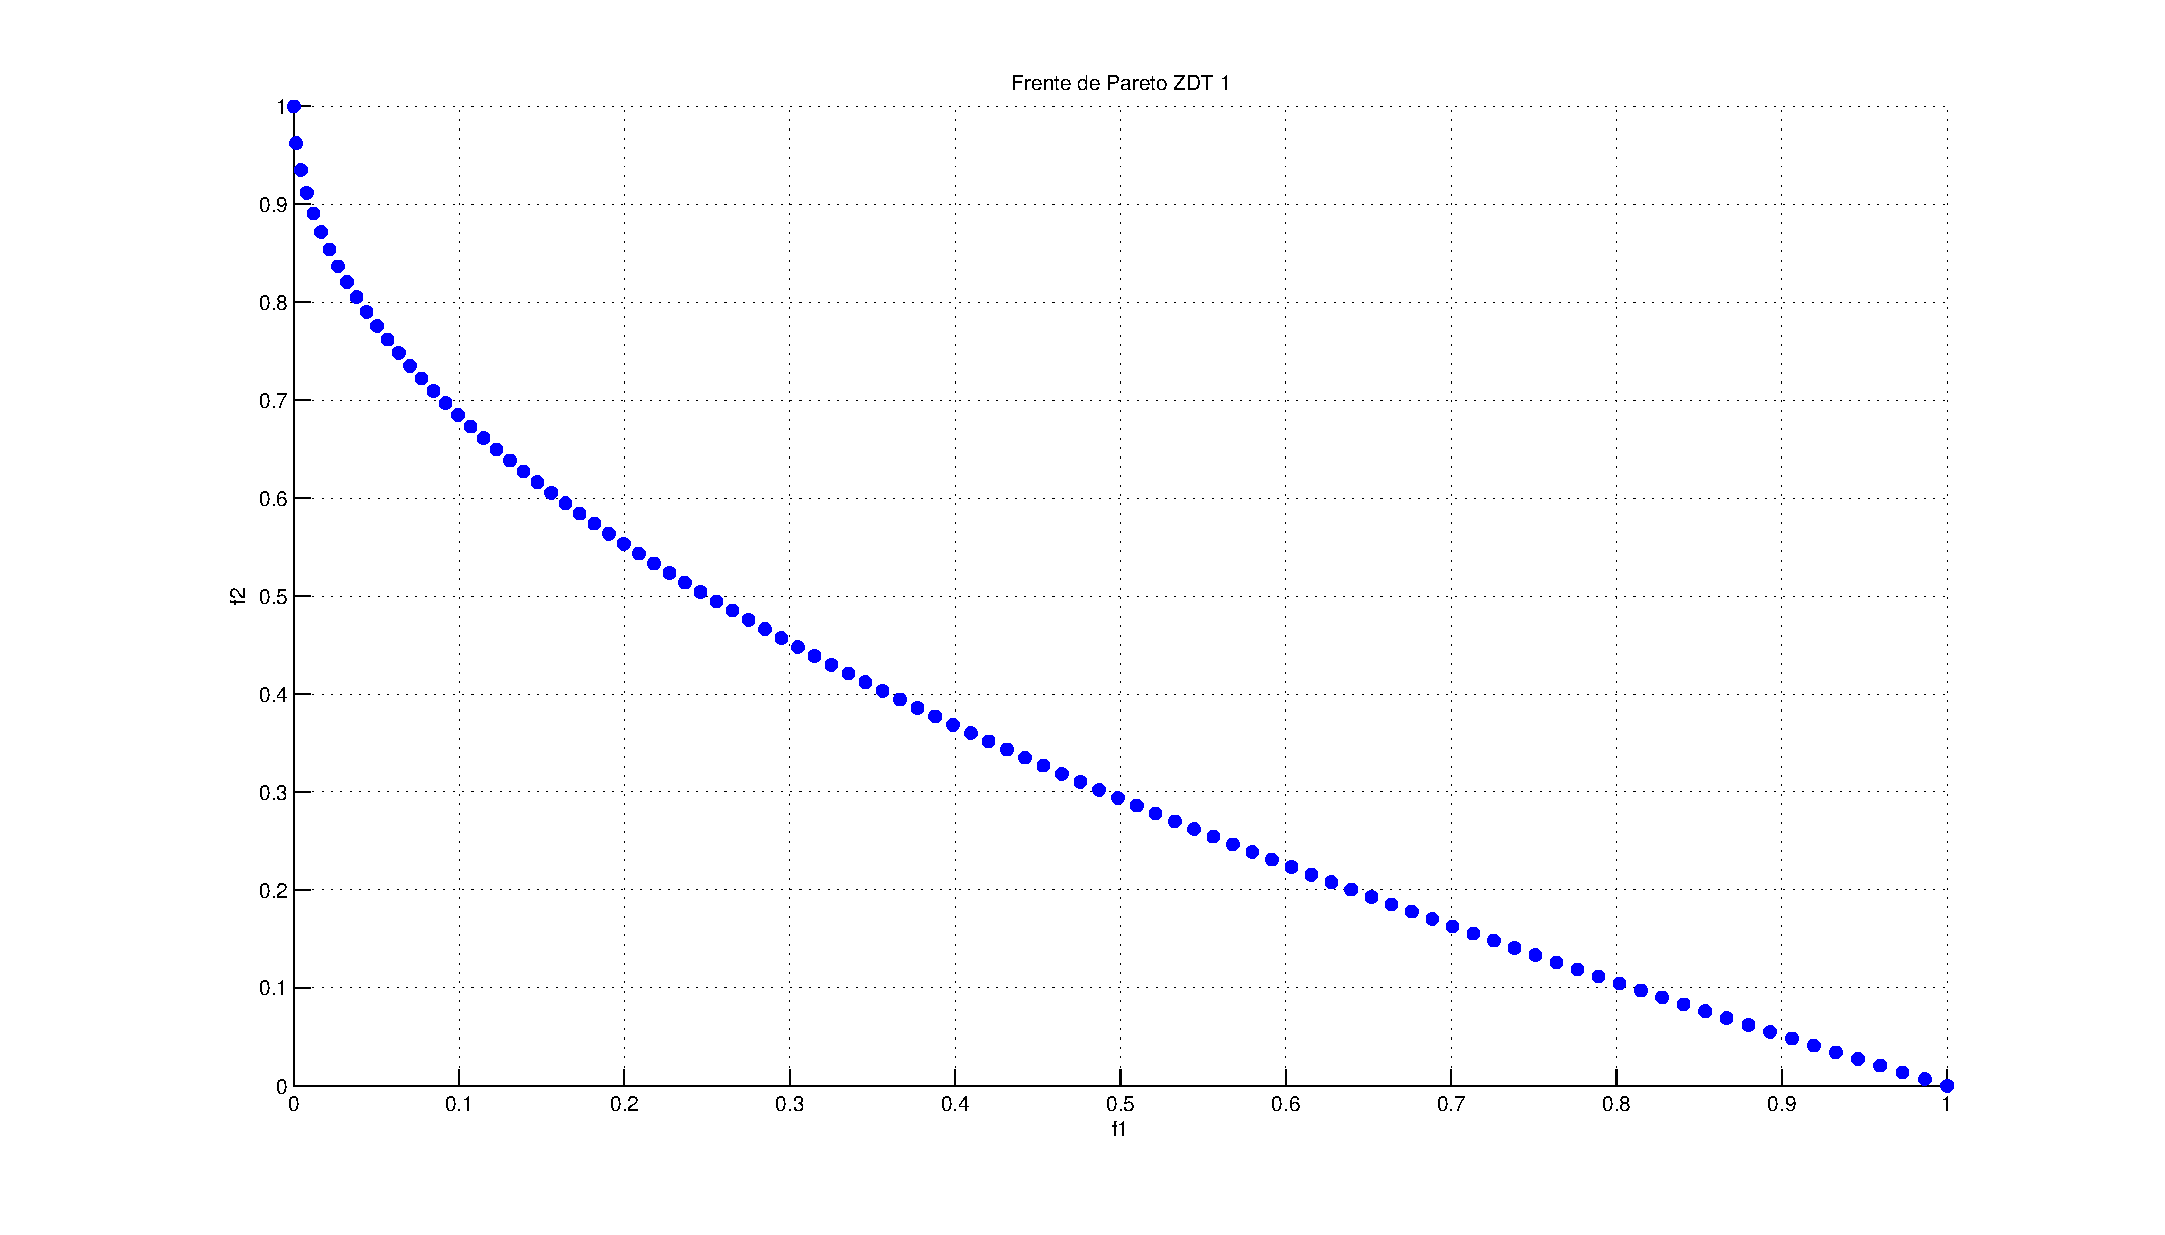
\includegraphics[scale=0.4]{ApendiceA/paretoZDT1.eps}
    \caption{Frente de Pareto verdadero de ZDT1}
    \label{fig:zdt1}
\end{figure}
 
\begin{figure}
\centering
 
    \centering
    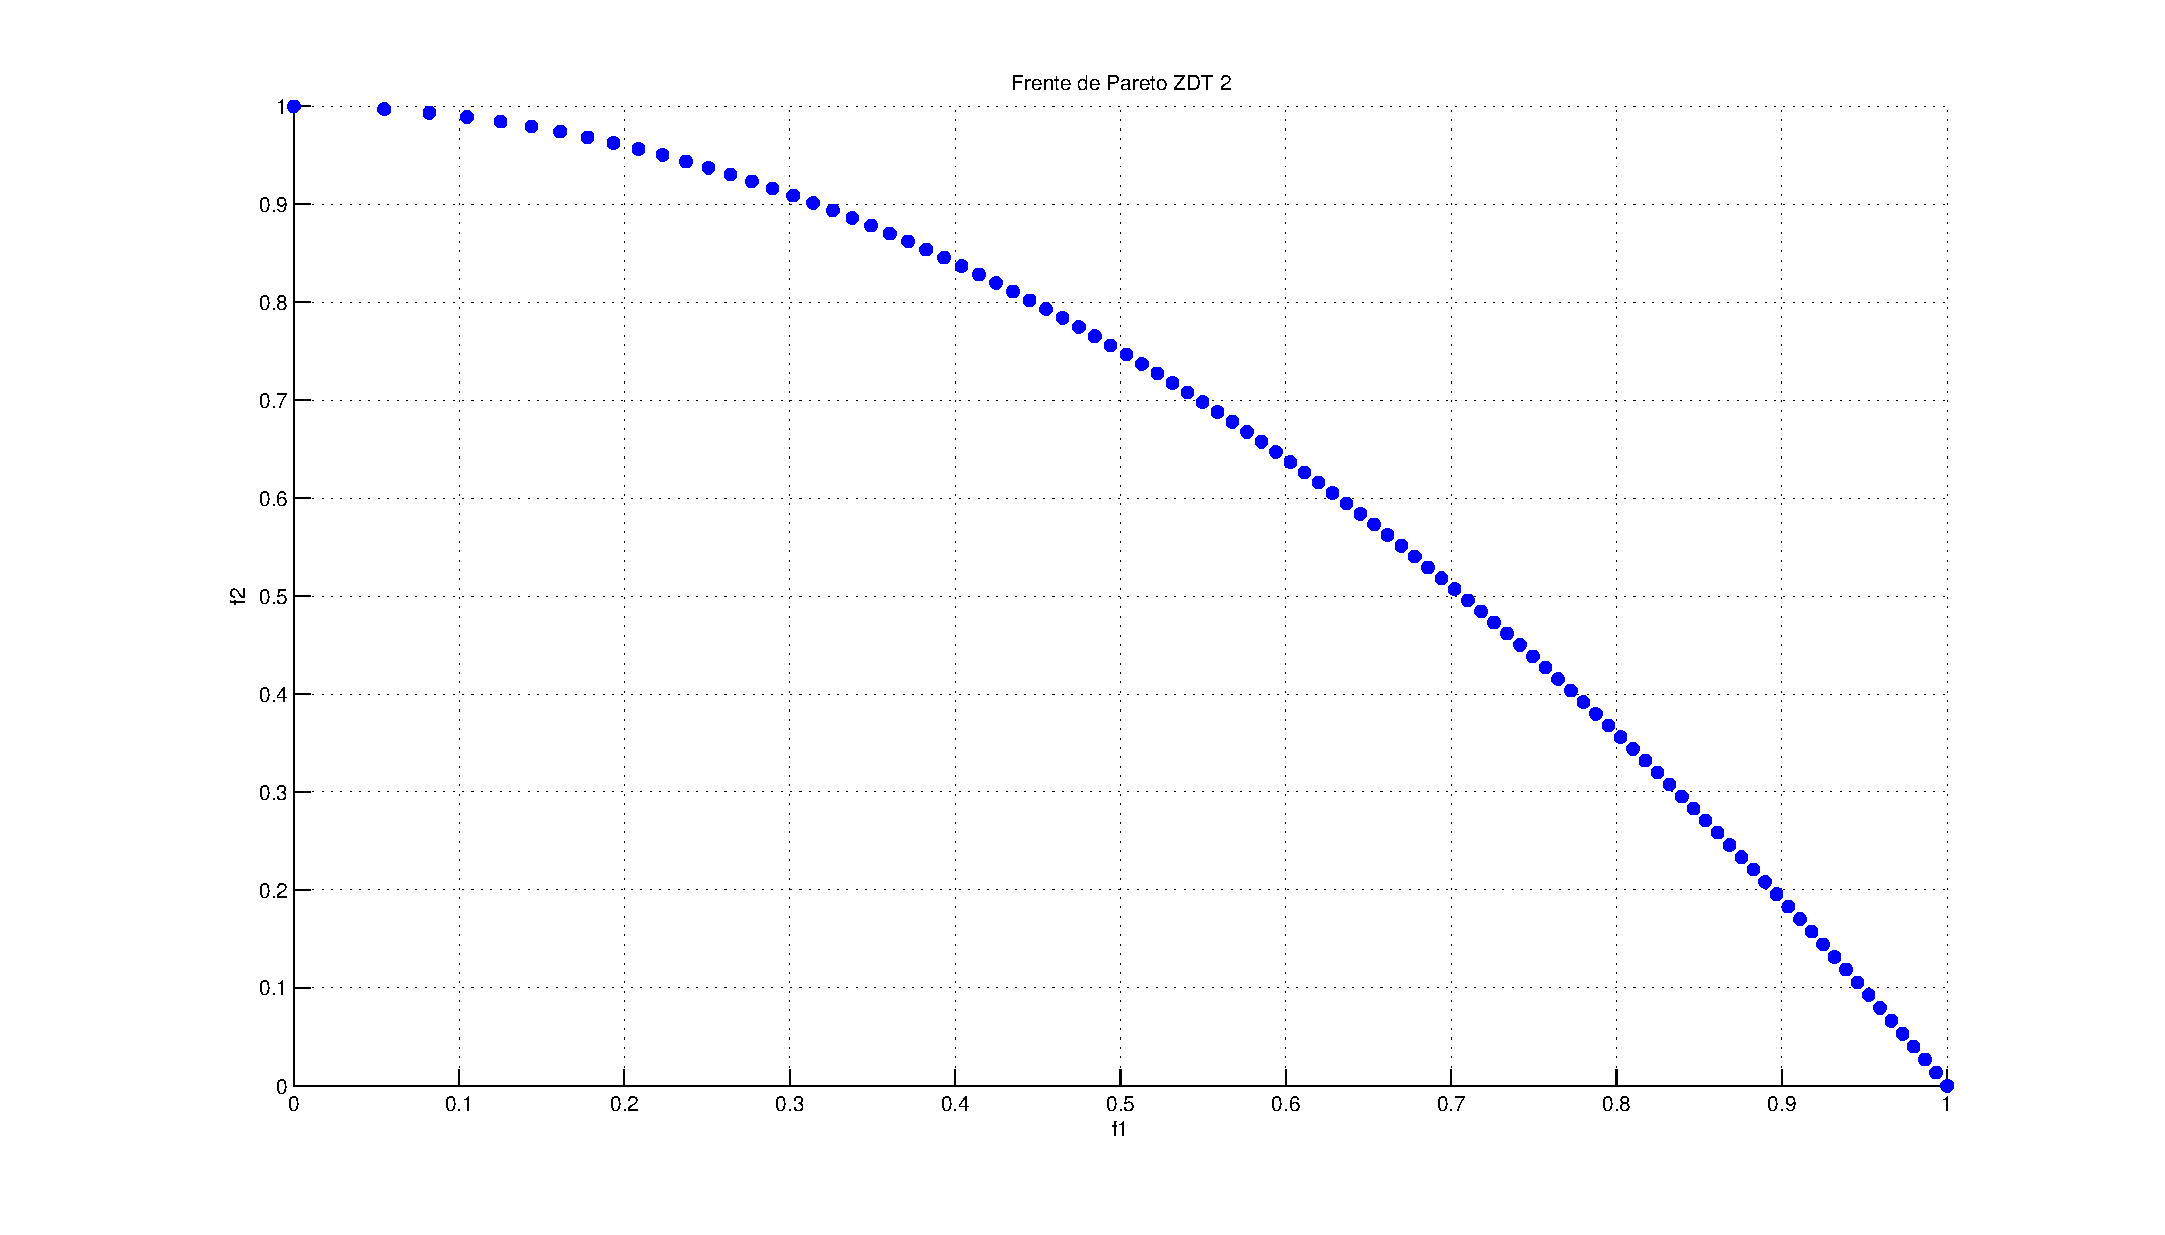
\includegraphics[scale=0.4]{ApendiceA/paretoZDT2.eps}
    \caption{Frente de Pareto verdadero de ZDT2}
    \label{fig:zdt2}
\end{figure}

\begin{figure}
\centering
    \centering
    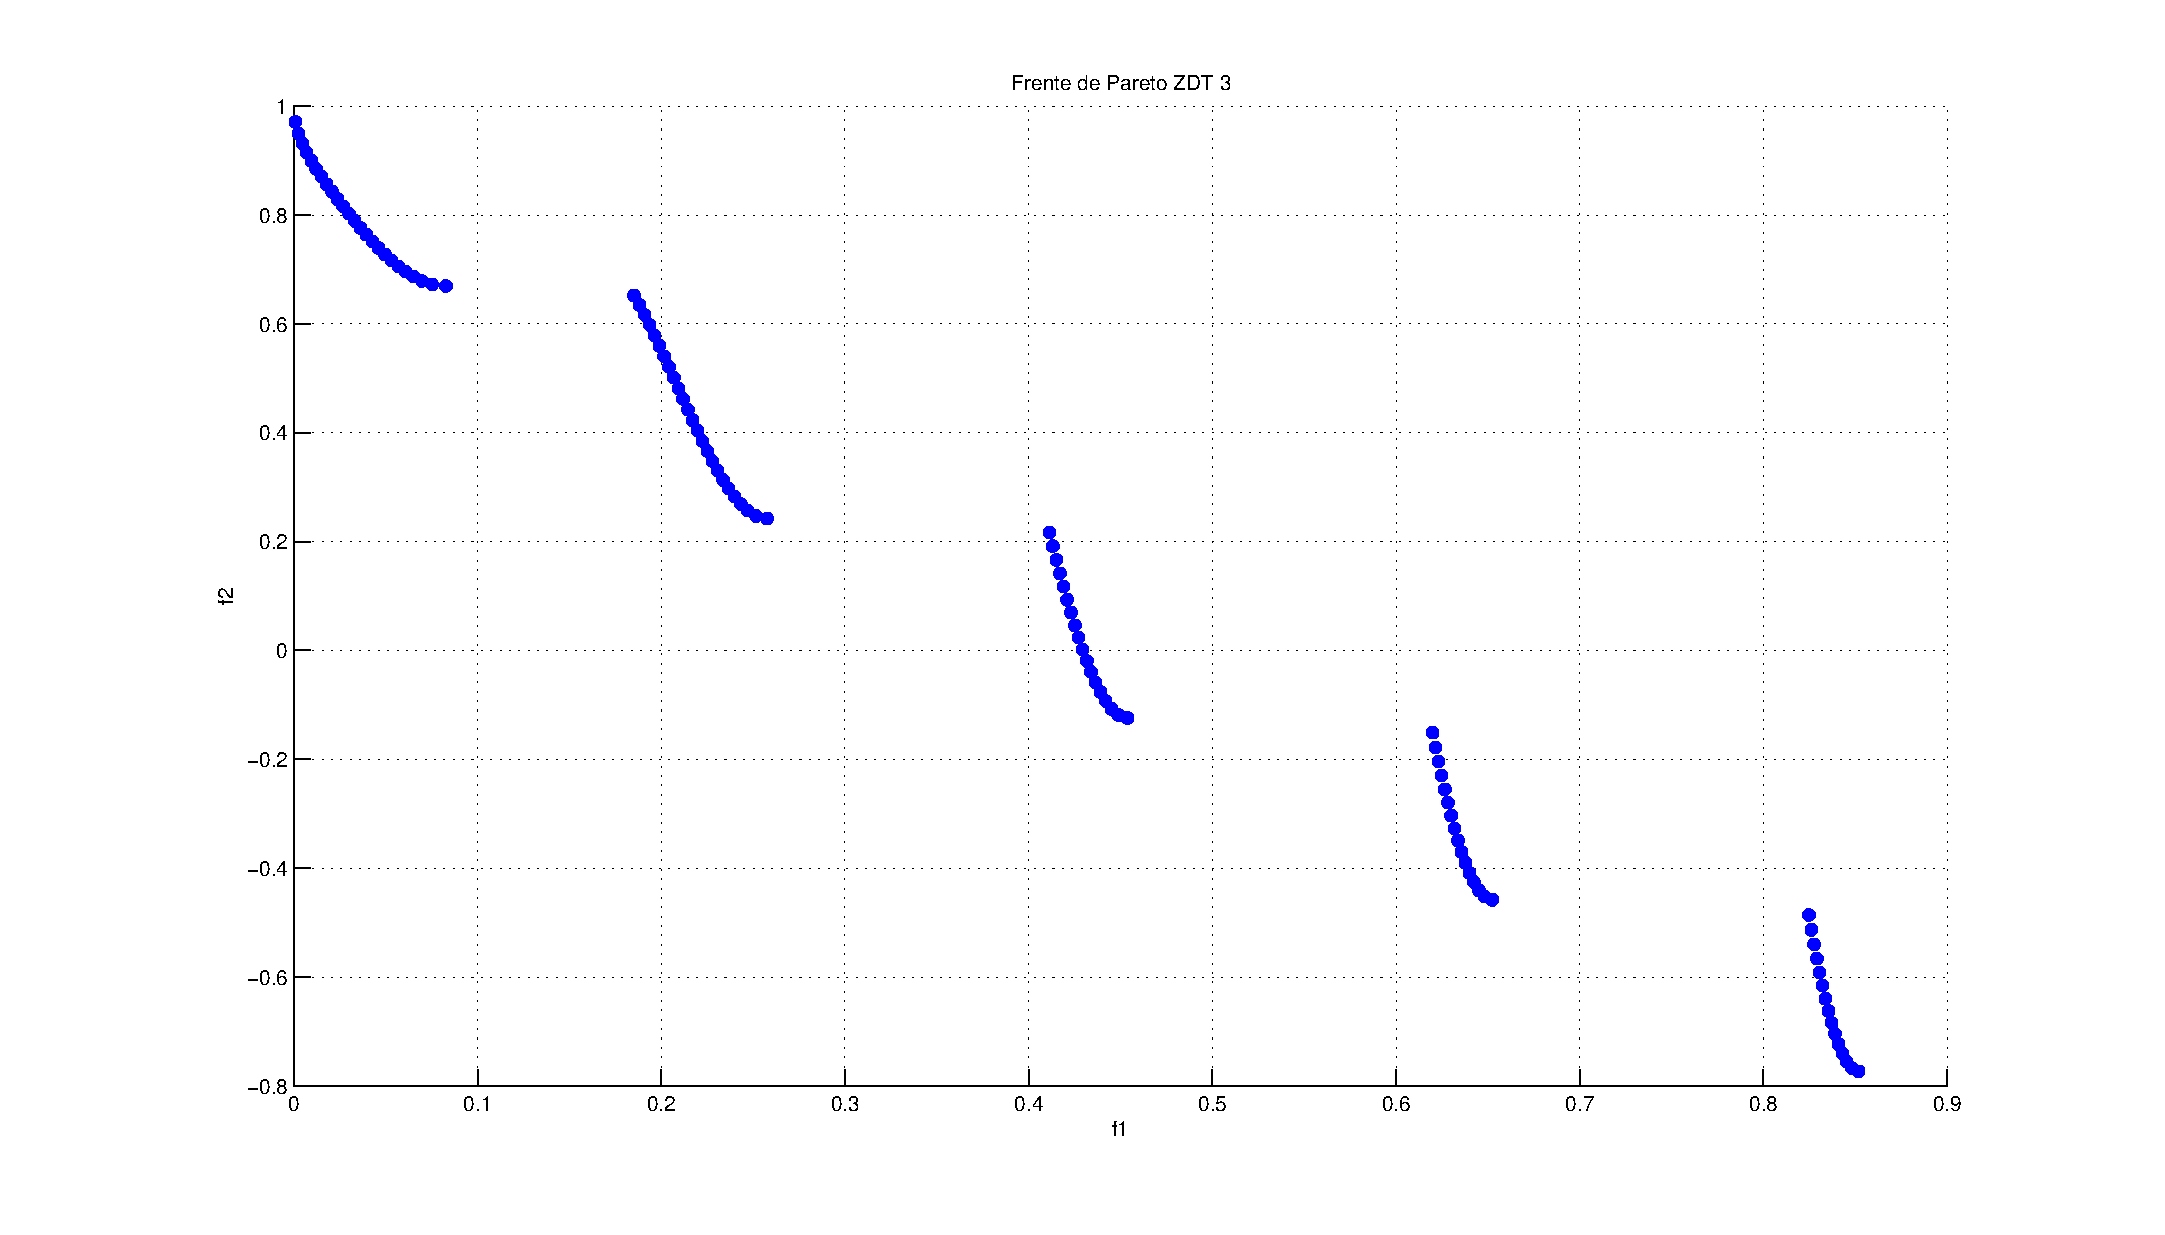
\includegraphics[scale=0.4]{ApendiceA/paretoZDT3.eps}
    \caption{Frente de Pareto verdadero de ZDT3}
    \label{fig:zdt3}
\end{figure}

\begin{figure}
\centering
    \centering
    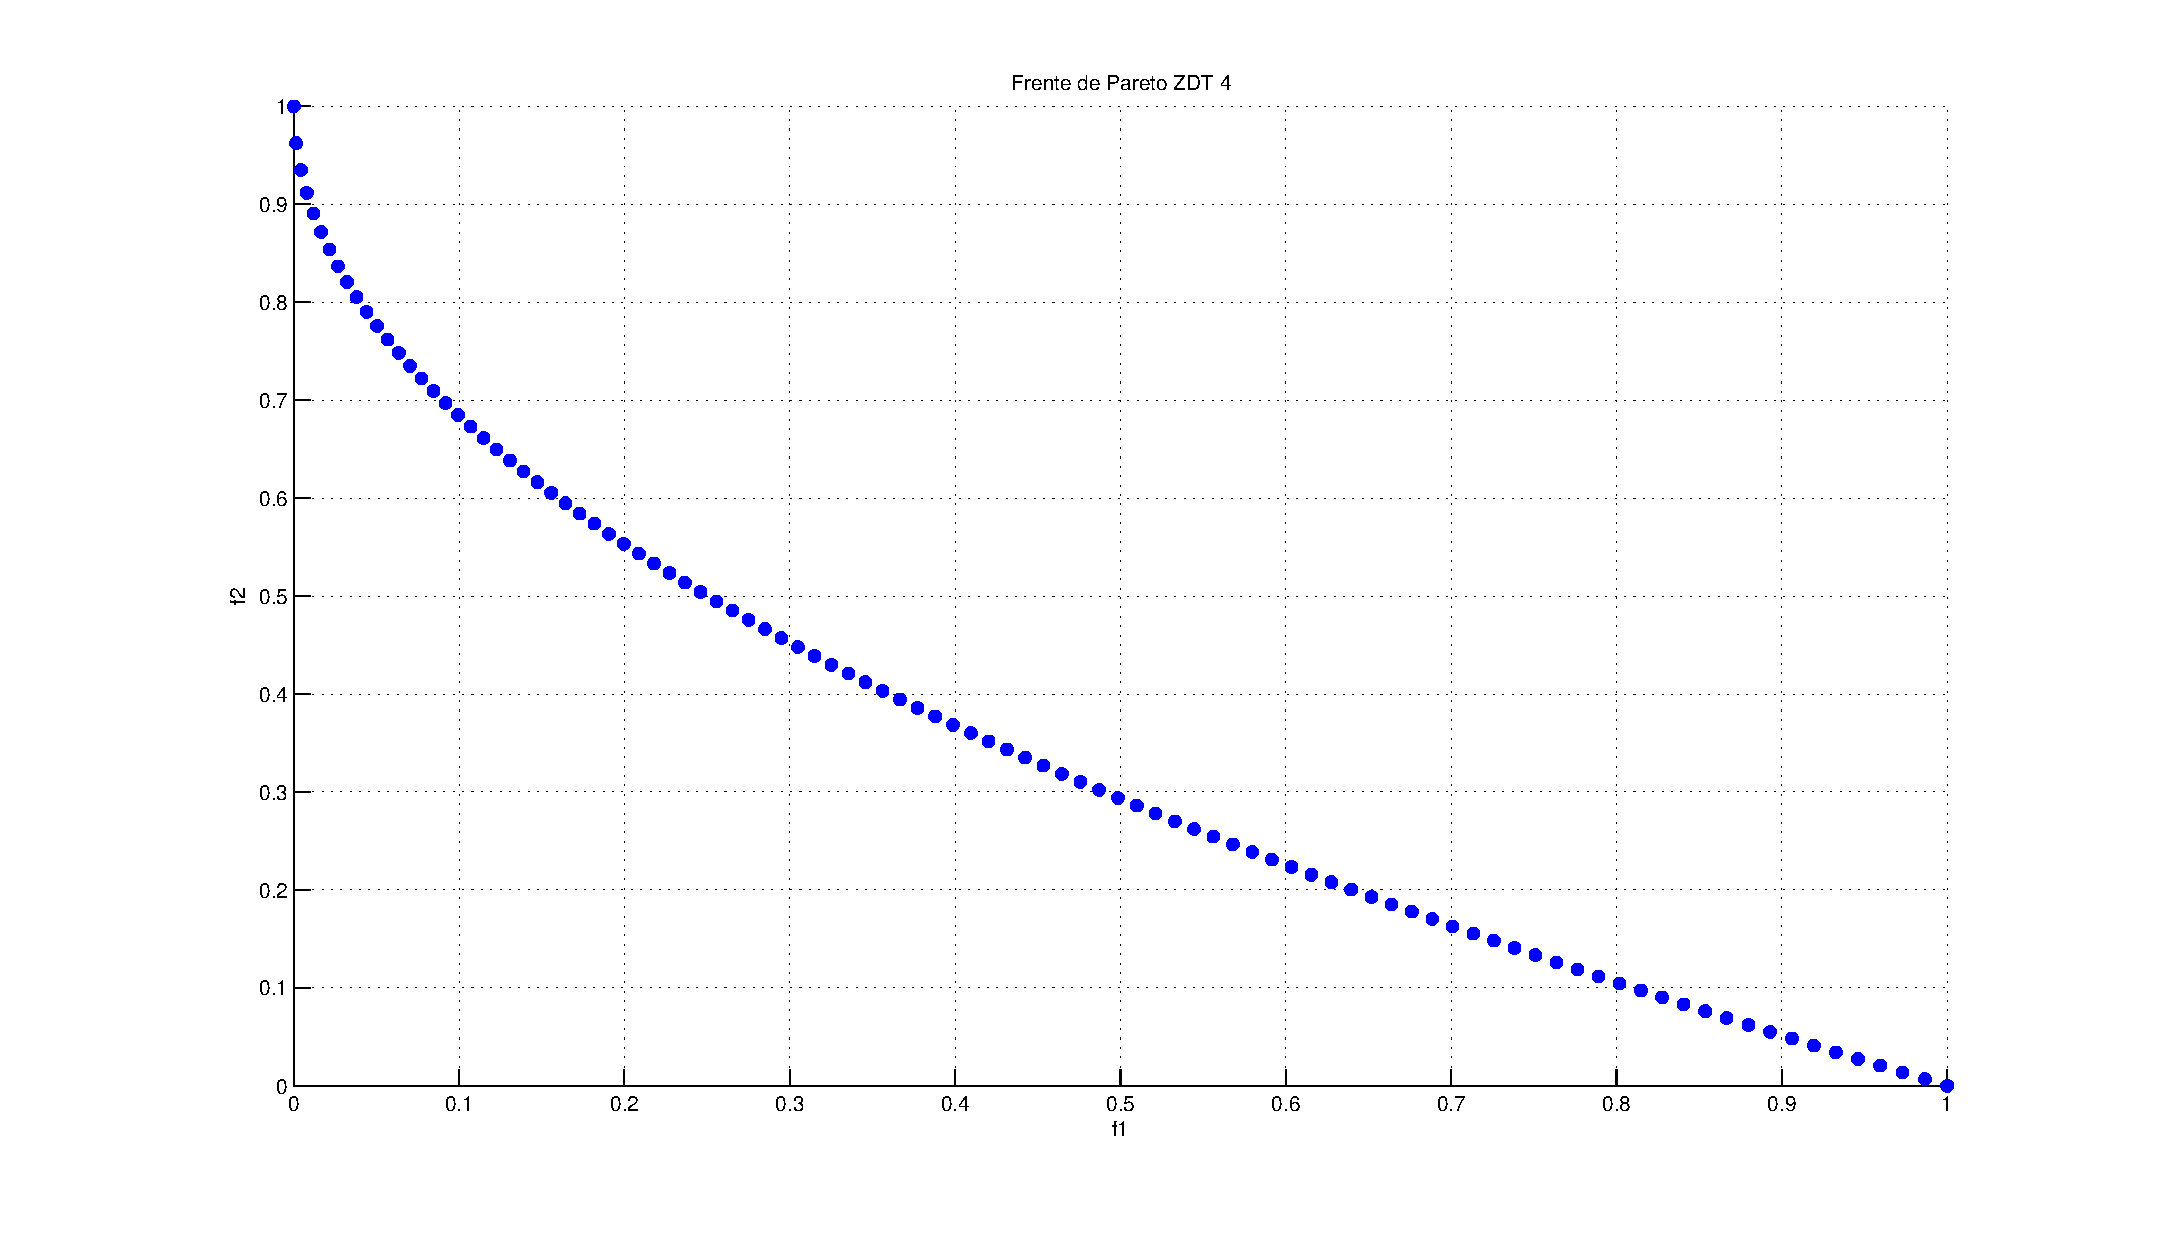
\includegraphics[scale=0.4]{ApendiceA/paretoZDT4.eps}
    \caption{Frente de Pareto verdadero de ZDT4}
    \label{fig:zdt4}
\end{figure}
\begin{figure}
\centering
    \centering
    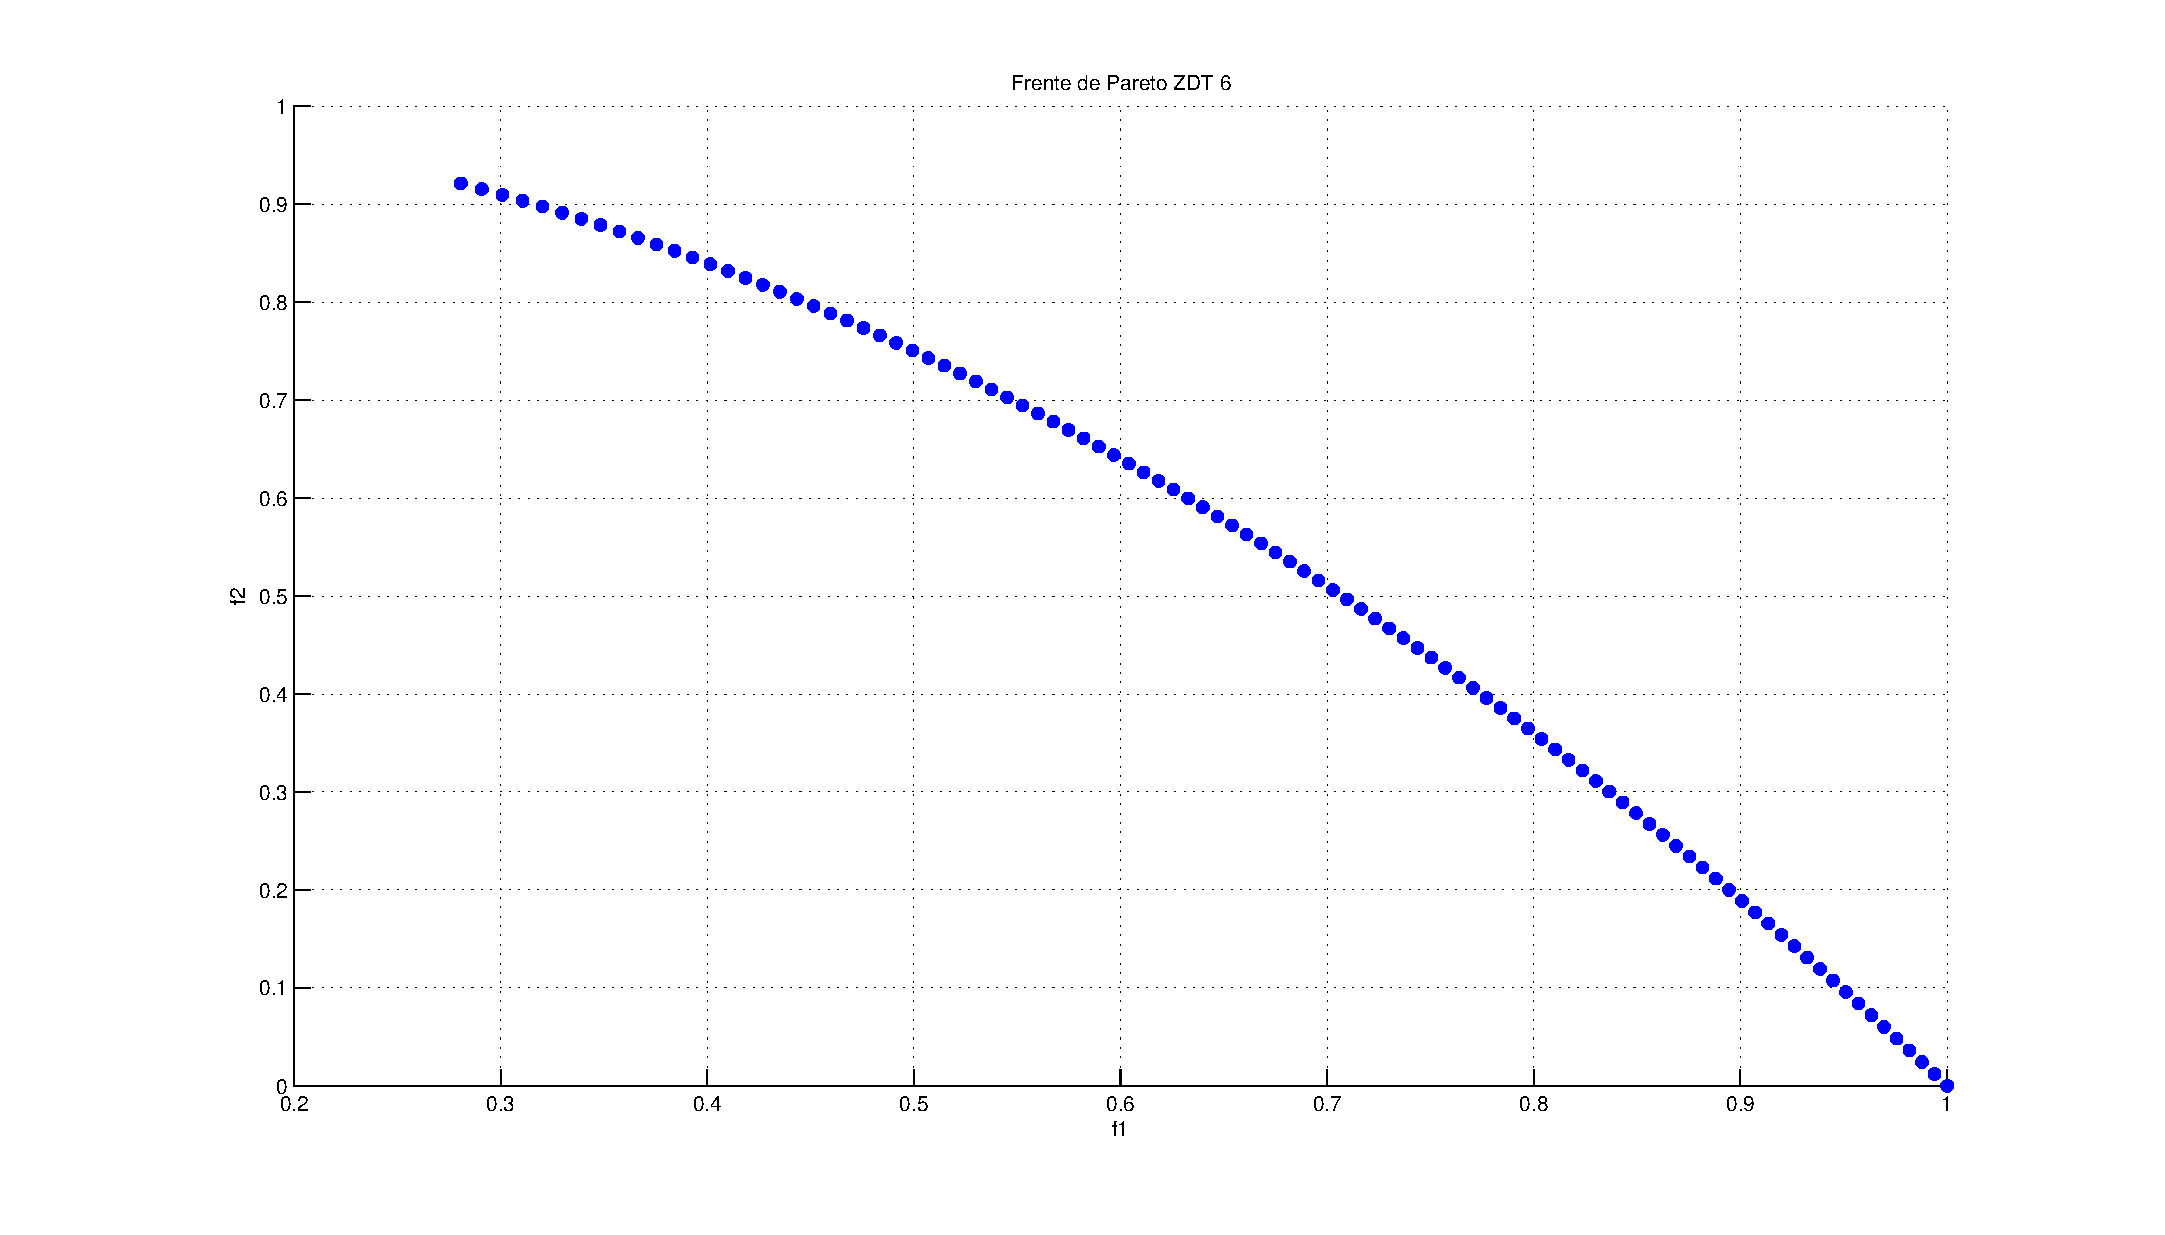
\includegraphics[scale=0.4]{ApendiceA/paretoZDT6.eps}
    \caption{Frente de Pareto verdadero de ZDT6}
    \label{fig:zdt6}
 
\end{figure}

\newpage
\section{Evaluaci\'on del conjunto de problemas ZDT}
  La comparaci\'on de los resultados de cada algoritmo se realiz\'o con los valores promedio obtenidos por cada m\'etrica.
  El punto de referencia utilizado en cada caso para el indicador del hipervolumen se muestra en la tabla \ref{tab:ref}.
  
  Los resultados obtenidos para los primeros tres problemas ZDT son similares para a mayoria de los resultados. 
  Donde el SMS-EMOA resulta ganador en la mayor parte de las m\'etricas convergencia seguido por nuestra propuesta (MOPSOhv), 
  como se muestra en las tablas \ref{tab:zdt1}, \ref{tab:zdt2} y \ref{tab:zdt3}. Sin embargo, nuestra propuesta 
  dominada a las soluciones del NSGA-II y MOPSOcd excepto al SMS-EMOA, de acuerdo a la m\'etrica de cobertura.
  
  Conforme a estos resultados se tiene una jerarqu\'ia en orden descendente en t\'erminos de convergencia en estos primeros tres 
  problemas:

\begin{enumerate}
  \item SMS-EMOA
  \item MOPSOhv
  \item NSGA-II
  \item MOPSOcd
\end{enumerate}
  
  En estos problemas puede verse que, se tienen dos casos especiales (ZDT4 y ZDT6). 
  
  El problema ZDT4 tiene un frente de Pareto que es altamente multifrontal el cual consiste en $21^9$ frentes de Paretos locales.
  Nuestra propuesta (MOPSOhv) no es capaz de generar buenas soluciones del frente quedando rezagado ligeramente por el SMS-EMOA y el NSGA-II
  (como muestra la tabla \ref{tab:zdt4}). Sin embargo,
  obtiene, en general, mejores resultados en la m\'etrica de cobertura las soluciones obtenidas por el SMS-EMOA y marginalmente 
  peores que los del NSGA-II. Los resultados gr\a'ficas obtenidas por el algoritmo MOPSOcd muestran que queda atrapado en un frente de Pareto 
  local, por lo que, nuestra propuesta es mejor. 
  
  Los resultados gr\'aficos de las figuras \ref{fig:zdt1}, \ref{fig:zdt2} y \ref{fig:zdt3} muestran que el SMS-EMOA se distribuye 
  mejor en la mayoria de esto problemas seguido por nuestra propuesta (MOPSOhv). En la figura \ref{fig:zdt4} muestra como el
  MOPSOcd queda atrapado en un frete de Pareto local.  
  
  El problema ZDT6 presenta un espacio de b\'usqueda no uniforme. Los resultados obtenidos por nuestra propuesta (MOPSOhv) son ligeramente 
  superados por los obtenidos por el SMS-EMOA y el NSGA-II. Debido a la baja densidad de las soluciones obtenidas por el algoritmo 
  MOPSOcd como se muestra en la figura \ref{fig:zdt6} no es capaz de alcanzar una buena aproximaci\'on al frente de Pareto real, por 
  lo que, nuestra propuesta es mejor.
  
   Conforme a estos resultados se tiene una jerarqu\'ia en orden descendente en t\'erminos de convergencia en estos \'ultimos dos 
  problemas:
  
  \begin{enumerate}
  \item NSGA-II
  \item SMS-EMOA
  \item MOPSOhv
  \item MOPSOcd
\end{enumerate}

  
  En general, las soluciones obtenidas por nuestra propuesta (MOPSOhv), para el conjunto de problemas ZDT, quedan entre las soluciones 
  obtenidas por SMS-EMOA y el NSGA-II, y siendo mejores que las soluciones obtenidas por el MOPSOcd.
	
  Los resultados se muestran de la siguiente forma: el color negro para el mejor valor, el color azul para el segundo, el color 
  verde para el tercero y el color rojo para la peor valor de las m\'etricas.

\begin{table}
  \begin{center}
    \begin{tabular}{|l||c|}
	\hline
	Problema  & Punto de referencia \\ 
	\hline
	\hline
	ZDT1 & $(1.1,1.1)$ \\ 
	\hline
	ZDT2 &  $(1.1,1.1)$\\
	\hline
	ZDT3 &  $(1.1,1.1)$\\
	\hline
	ZDT4 &  $(0.9,1.1)$\\
	\hline
	ZDT6 &  $(1.1,1.1)$\\
	\hline
  \end{tabular}
  \caption{Puntos de referencia utilizados para el conjunto de problemas ZDT}
  \label{tab:ref}
\end{center}
\end{table}

\newpage

 \begin{table}
 \begin{center}
  \begin{tabular}{|l||cc|cc|} \hline
    & \multicolumn{4}{|c|}{\textbf{Espaciado}} \\     
	\textbf{Algoritmo} & \textbf{Menor} & \textbf{Mayor} & \textbf{Promedio} & \textbf{Desviaci\'on} \\  \hline \hline
	\textbf{MOPSOhv} &0.003157 & 0.004218 & \textbf{\textcolor{blue}{0.003524}} & \textbf{\textcolor{blue}{0.000305}}  \\ 
	\textbf{MOPSOcd} &0.006072 & 0.007475 & \textbf{\textcolor{green}{0.006962}} & \textbf{\textcolor{green}{0.000362}}  \\ 
	\textbf{NSGA-II} &0.005950 & 0.007813 & \textbf{\textcolor{red}{0.007020}} & \textbf{\textcolor{red}{0.000447}}   \\  
	\textbf{SMS-EMOA}&0.001840 & 0.002976 & \textbf{0.002320} & \textbf{0.000270}  \\  
	\hline\hline
    & \multicolumn{4}{|c|}{\textbf{DGI}} \\  \hline \hline
	\textbf{MOPSOhv} &0.017011 & 0.017021 & \textbf{\textcolor{green}{0.017014}} & \textbf{\textcolor{blue}{0.000003}}  \\ 
	\textbf{MOPSOcd} &0.017092 & 0.017240 & \textbf{\textcolor{red}{0.017173}} & \textbf{\textcolor{red}{0.000036}} \\ 
	\textbf{NSGA-II} &0.017008 & 0.017021 & \textbf{\textcolor{blue}{0.017011}} & \textbf{\textcolor{green}{0.000003}} \\  
	\textbf{SMS-EMOA}&0.017008 & 0.017010 & \textbf{0.017009} & \textbf{0.000001}   \\  
	\hline\hline
    & \multicolumn{4}{|c|}{\textbf{Hipervolumen}} \\ \hline\hline 
	\textbf{MOPSOhv} &0.871620 & 0.871991 & \textbf{\textcolor{blue}{0.871849}} & \textbf{\textcolor{blue}{0.000095}}  \\ 
	\textbf{MOPSOcd} &0.861718 & 0.868142 & \textbf{\textcolor{red}{0.864645}} & \textbf{\textcolor{red}{0.001562}} \\ 
	\textbf{NSGA-II} &0.870107 & 0.871006 & \textbf{\textcolor{green}{0.870461}} & \textbf{\textcolor{green}{0.000206}} \\  
	\textbf{SMS-EMOA}&0.872115 & 0.872134 & \textbf{0.872129} & 0.000006 \\  
	\hline\hline
   & \multicolumn{4}{|c|}{\textbf{Cobertura}} \\ \hline\hline 
	\textbf{Algoritmo} & \textbf{MOPSOhv} & \textbf{MOPSOcd} & \textbf{NSGA-II} & \textbf{SMS-EMOA} \\  \hline \hline
	\textbf{MOPSOhv} & ---      & \textbf{0.722500}  & \textbf{0.074500} & \textbf{\textcolor{red}{0.000001}}  \\ 
	\textbf{MOPSOcd} & 0.000001 & ---       & 0.005500 & 0.000001 \\ 
	\textbf{NSGA-II} & 0.022500 & 0.618000  & ---      & 0.013500 \\  
	\textbf{SMS-EMOA}& \textbf{0.028500} & 0.762500  & 0.053500 & --- \\  
	\hline
	\end{tabular}
    \caption{Resultados correspondientes al problema ZDT1.}
  \label{tab:zdt1}
\end{center}
\end{table}

La convergencia y la distribuci\'on de las soluciones de nuestra propuesta (MOPSOhv) es buena para este problema, seguido por el SMS-EMOA 
que presenta la mejor convergencia y distribuci\'on (como se muestra en la tabla \ref{tab:zdt1}). Conforme a estos resultados se puede crear una
jerarqu\'ia en orden descendente en t\'erminos de convergencia del conjunto de soluciones pr\'oximas al frente de Pareto real:

\begin{enumerate}
  \item SMS-EMOA
  \item MOPSOhv
  \item NSGA-II
  \item MOPSOcd
\end{enumerate}

Tambi\'en, se observa que en las soluciones de nuestra propuesta dominan a las soluciones del NSGA-II y MOPSOcd, y siendo superado por las 
soluciones del SMS-EMOA.

\newpage
    \begin{figure}
      \centering
	%\begin{rotate}{0}
	  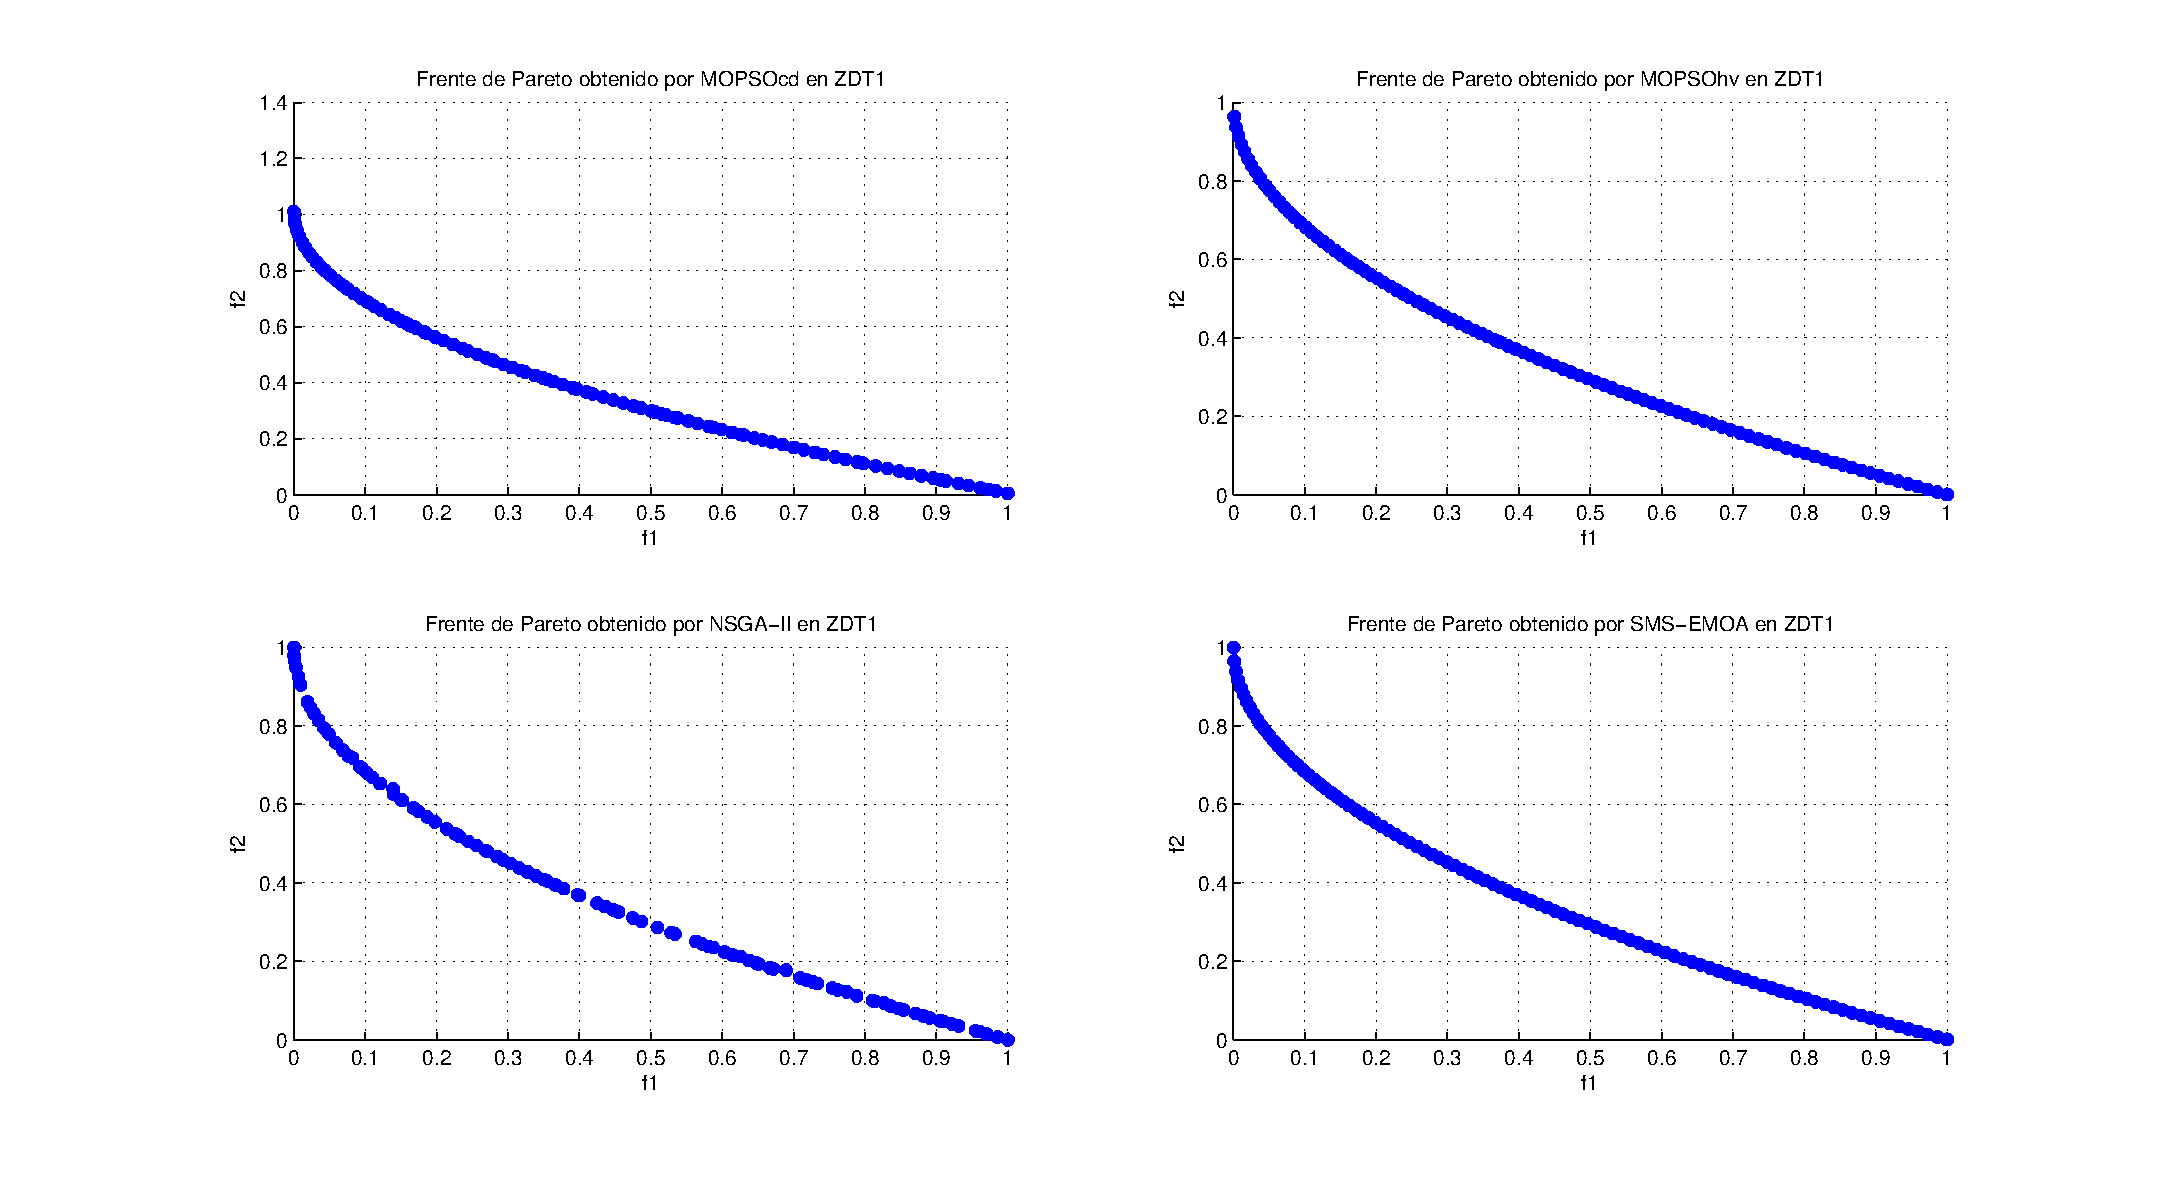
\includegraphics[scale=0.45]{Cap4/rzdt1r.eps}      
%	  \end{rotate}
	\caption{Resultados gr\'aficos correspondientes al problema ZDT1.}
      \label{fig:rZDT1}
      \end{figure}
\clearpage

\newpage
 \begin{table}
 \begin{center}
  \begin{tabular}{|l|cc|cc|} \hline
    & \multicolumn{4}{|c|}{\textbf{Espaciado}} \\ 
	\textbf{Algoritmo} & \textbf{Menor} & \textbf{Mayor} & \textbf{Promedio} & \textbf{Desviaci\'on} \\  \hline\hline
	\textbf{MOPSOhv} &0.004345 & 0.005129 & \textbf{\textcolor{blue}{0.004679}} & \textbf{0.000217}  \\ 
	\textbf{MOPSOcd} &0.006054 & 0.007826 & \textbf{\textcolor{red}{0.007014}} &  \textbf{\textcolor{blue}{0.0005170}}\\ 
	\textbf{NSGA-II} &0.006027 & 0.008074 & \textbf{\textcolor{green}{0.006956}} & \textbf{\textcolor{red}{ 0.000610}}  \\  
	\textbf{SMS-EMOA}&0.002167 & 0.004664 & \textbf{0.004063} & \textbf{\textcolor{green}{0.000543}}  \\  
	\hline\hline
    & \multicolumn{4}{|c|}{\textbf{DGI}} \\ \hline \hline	
	\textbf{MOPSOhv} &0.027389 & 0.027394 & \textbf{\textcolor{green}{0.027391}}& \textbf{\textcolor{green}{0.000001}}  \\ 
	\textbf{MOPSOcd} &0.027462 & 0.027521 & \textbf{\textcolor{red}{0.027497}}  & \textbf{\textcolor{red}{0.000015}}  \\ 
	\textbf{NSGA-II} &0.027386 & 0.027389 & \textbf{\textcolor{blue}{0.027387}} & \textbf{\textcolor{blue}{0.000001}}  \\  
	\textbf{SMS-EMOA}&0.027386 & 0.027387 & \textbf{0.027386} &\textbf{0.000000 } \\  
	\hline\hline
    & \multicolumn{4}{|c|}{\textbf{Hipervolumen}} \\ 	\hline \hline
	\textbf{MOPSOhv} &0.538426 & 0.538666 & \textbf{\textcolor{blue}{0.538568}} & \textbf{\textcolor{blue}{0.000058}} \\ 
	\textbf{MOPSOcd} &0.530732 & 0.534137 & \textbf{\textcolor{red}{0.532098}}  & \textbf{\textcolor{red}{0.000882}}   \\ 
	\textbf{NSGA-II} &0.537163 & 0.537699 & \textbf{\textcolor{green}{0.537424}}& \textbf{\textcolor{green}{0.000148}}  \\  
	\textbf{SMS-EMOA}&0.538808 & 0.538879 & \textbf{0.538872} & \textbf{0.000015}  \\  
	\hline\hline
    & \multicolumn{4}{|c|}{\textbf{Cobertura}} \\ \hline\hline 
	\textbf{Algoritmo} & \textbf{MOPSOhv} & \textbf{MOPSOcd} & \textbf{NSGA-II} & \textbf{SMS-EMOA} \\  \hline \hline
	\textbf{MOPSOhv} &---       &\textbf{0.637500} & \textbf{0.044000}  & \textbf{\textcolor{red}{0.000500}} \\ 
	\textbf{MOPSOcd} & 0.000001 & ---      & 0.003500  & 0.000500 \\ 
	\textbf{NSGA-II} & 0.036500 & 0.589500 & ---      & 0.017500  \\  
	\textbf{SMS-EMOA}& \textbf{0.026500} & 0.665000 & 0.034000 & --- \\  
	\hline
	\end{tabular}
  \caption{Resultados correspondientes al problema ZDT2.}
  \label{tab:zdt2}
\end{center}
\end{table}

La convergencia y la distribuci\'on de las soluciones de nuestra propuesta (MOPSOhv) es buena para este problema, seguido por el SMS-EMOA 
que presenta la mejor convergencia y distribuci\'on (como se muestra en la tabla \ref{tab:zdt2}). Conforme a estos resultados se puede crear una
jerarqu\'ia en orden descendente en t\'erminos de convergencia del conjunto de soluciones pr\'oximas al frente de Pareto real:

\begin{enumerate}
  \item SMS-EMOA
  \item MOPSOhv
  \item NSGA-II
  \item MOPSOcd
\end{enumerate}

Tambi\'en, se observa que en las soluciones de nuestra propuesta dominan a las soluciones del NSGA-II y MOPSOcd, y siendo superado por las 
soluciones del SMS-EMOA.

\clearpage
\newpage
\begin{figure}
      \begin{center}
	  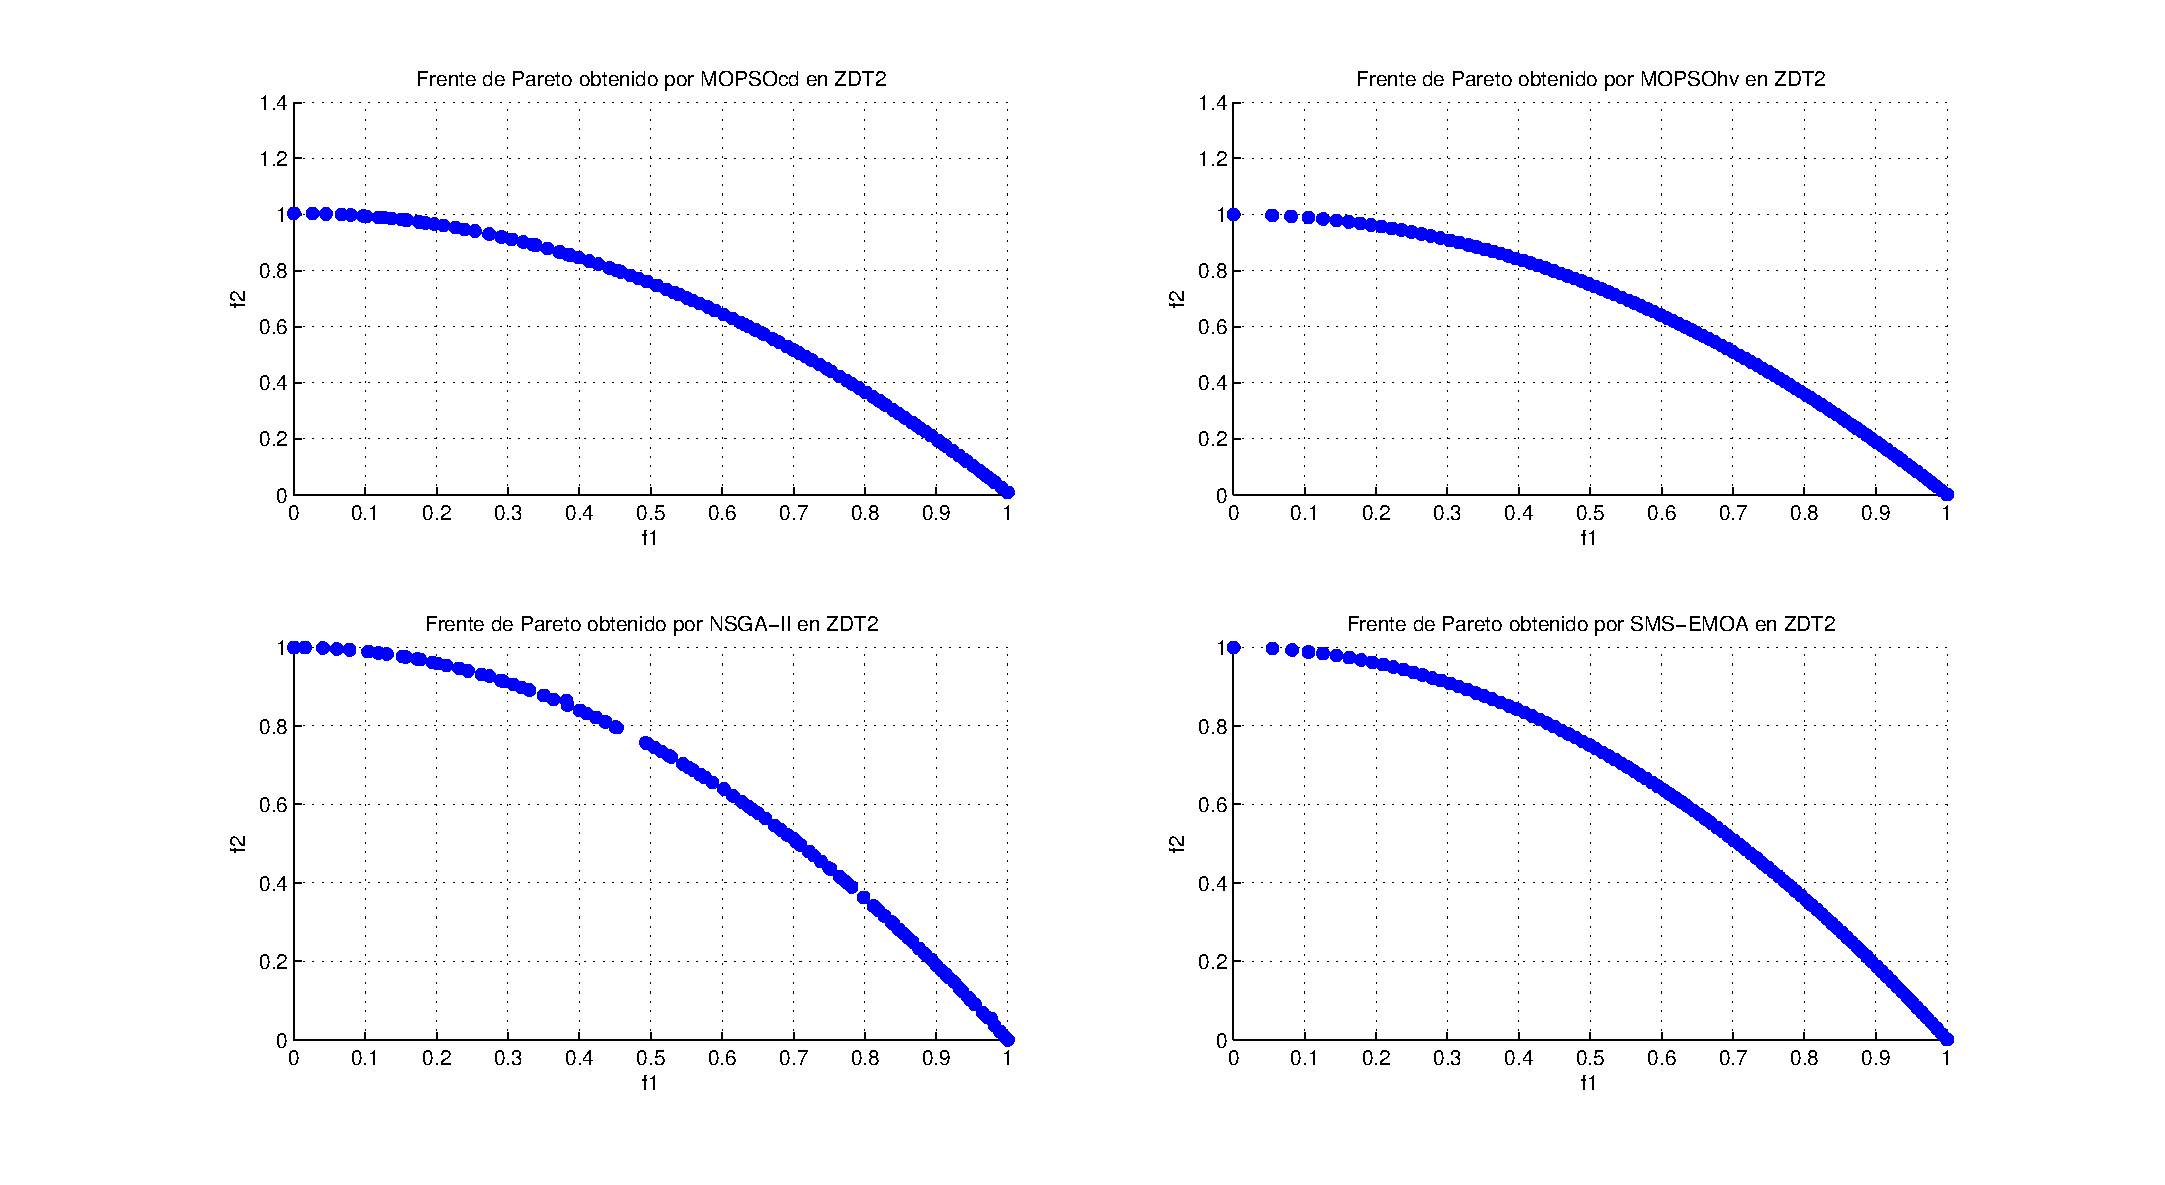
\includegraphics[scale=0.45]{Cap4/rzdt2r.eps}
      \end{center}
	\caption{Resultados gr\'aficos correspondientes al problema ZDT2.}
      \label{fig:rZDT2}
      \end{figure}
\clearpage
\newpage
 \begin{table}
 \begin{center}
  \begin{tabular}{|l|cc|cc|} \hline
    & \multicolumn{4}{|c|}{\textbf{Espaciado}} \\ 
	\textbf{Algoritmo} & \textbf{Menor} & \textbf{Mayor} & \textbf{Promedio} & \textbf{Desviaci\'on} \\  \hline\hline
	\textbf{MOPSOhv} &0.005672 & 0.006958 & \textbf{\textcolor{blue}{0.006248}} & \textbf{\textcolor{blue}{0.000328}}  \\ 
	\textbf{MOPSOcd} &0.007001 & 0.008605 & \textbf{\textcolor{green}{0.007656}}& \textbf{\textcolor{green}{0.000425}} \\ 
	\textbf{NSGA-II} &0.006809 & 0.009101 & \textbf{\textcolor{red}{0.007875}}  & \textbf{\textcolor{red}{0.000565}} \\  
	\textbf{SMS-EMOA}&0.001994 & 0.002563 & \textbf{0.002209} & \textbf{0.000165} \\  
	\hline\hline
    & \multicolumn{4}{|c|}{\textbf{DGI}} \\ 	\hline \hline
	\textbf{MOPSOhv} &0.011174 & 0.011219 & \textbf{\textcolor{blue}{0.011198}} & \textbf{\textcolor{green}{0.000012}} \\ 
	\textbf{MOPSOcd} &0.011389 & 0.011604 & \textbf{\textcolor{green}{0.011492}} & \textbf{\textcolor{red}{0.000064}} \\ 
	\textbf{NSGA-II} &0.011140 & 0.011184 & \textbf{0.011166} & \textbf{\textcolor{blue}{\textbf{0.000016}}} \\  
	\textbf{SMS-EMOA}&0.019892 & 0.019894 & \textbf{\textcolor{red}{0.019892}} & \textbf{0.000001} \\  
	\hline\hline
    & \multicolumn{4}{|c|}{\textbf{Hipervolumen}} \\ \hline \hline
	\textbf{MOPSOhv} &0.952055 & 0.953776 &\textbf{\textcolor{blue}{ 0.952907}} &\textbf{\textcolor{blue}{ 0.000452}}  \\ 
	\textbf{MOPSOcd} &0.936835 & 0.946304 &\textbf{\textcolor{green}{ 0.941991}} &\textbf{\textcolor{green}{ 0.002510}} \\ 
	\textbf{NSGA-II} &0.953544 & 0.954219 & \textbf{0.953912} & \textbf{0.000145}  \\  
	\textbf{SMS-EMOA}&0.522460 & 0.522466 &\textbf{\textcolor{red}{ 0.522464}} & \textbf{\textcolor{red}{0.000001}}  \\  
	\hline
    & \multicolumn{4}{|c|}{\textbf{Cobertura}} \\ \hline\hline 
	\textbf{Algoritmo} & \textbf{MOPSOhv} & \textbf{MOPSOcd} & \textbf{NSGA-II} & \textbf{SMS-EMOA} \\  \hline \hline
	\textbf{MOPSOhv} &---       & \textbf{0.637500} & \textbf{0.044000} & \textbf{\textcolor{red}{0.000500 }}\\ 
	\textbf{MOPSOcd} & 0.000001 & ---      & 0.003500 & 0.000500 \\ 
	\textbf{NSGA-II} & 0.036500 & 0.589500 & ---      & 0.017500 \\  
	\textbf{SMS-EMOA}& \textbf{0.026500} & 0.665000 & 0.034000 & --- \\  
	\hline\hline
	\end{tabular}
\caption{Resultados correspondientes al problema ZDT3.}
  \label{tab:zdt3}
\end{center}
\end{table}

La convergencia y la distribuci\'on de las soluciones de nuestra propuesta (MOPSOhv) es buena para este problema, seguido por el NSGA-II 
que presenta la mejor convergencia y el SMS-EMOA presenta la mejor distribuci\'on (como se muestra en la tabla \ref{tab:zdt3}). Conforme a 
estos resultados se puede crear una jerarqu\'ia en orden descendente en t\'erminos de convergencia del conjunto de soluciones pr\'oximas al 
frente de Pareto real:

\begin{enumerate}
  \item NSGA-II
  \item MOPSOhv
  \item MOPSOcd
  \item SMS-EMOA
\end{enumerate}

Tambi\'en, se observa que en las soluciones de nuestra propuesta dominan a las soluciones del NSGA-II y MOPSOcd, y siendo superado por las 
soluciones del SMS-EMOA.

\clearpage
\newpage
\begin{figure}
      \begin{center}
	  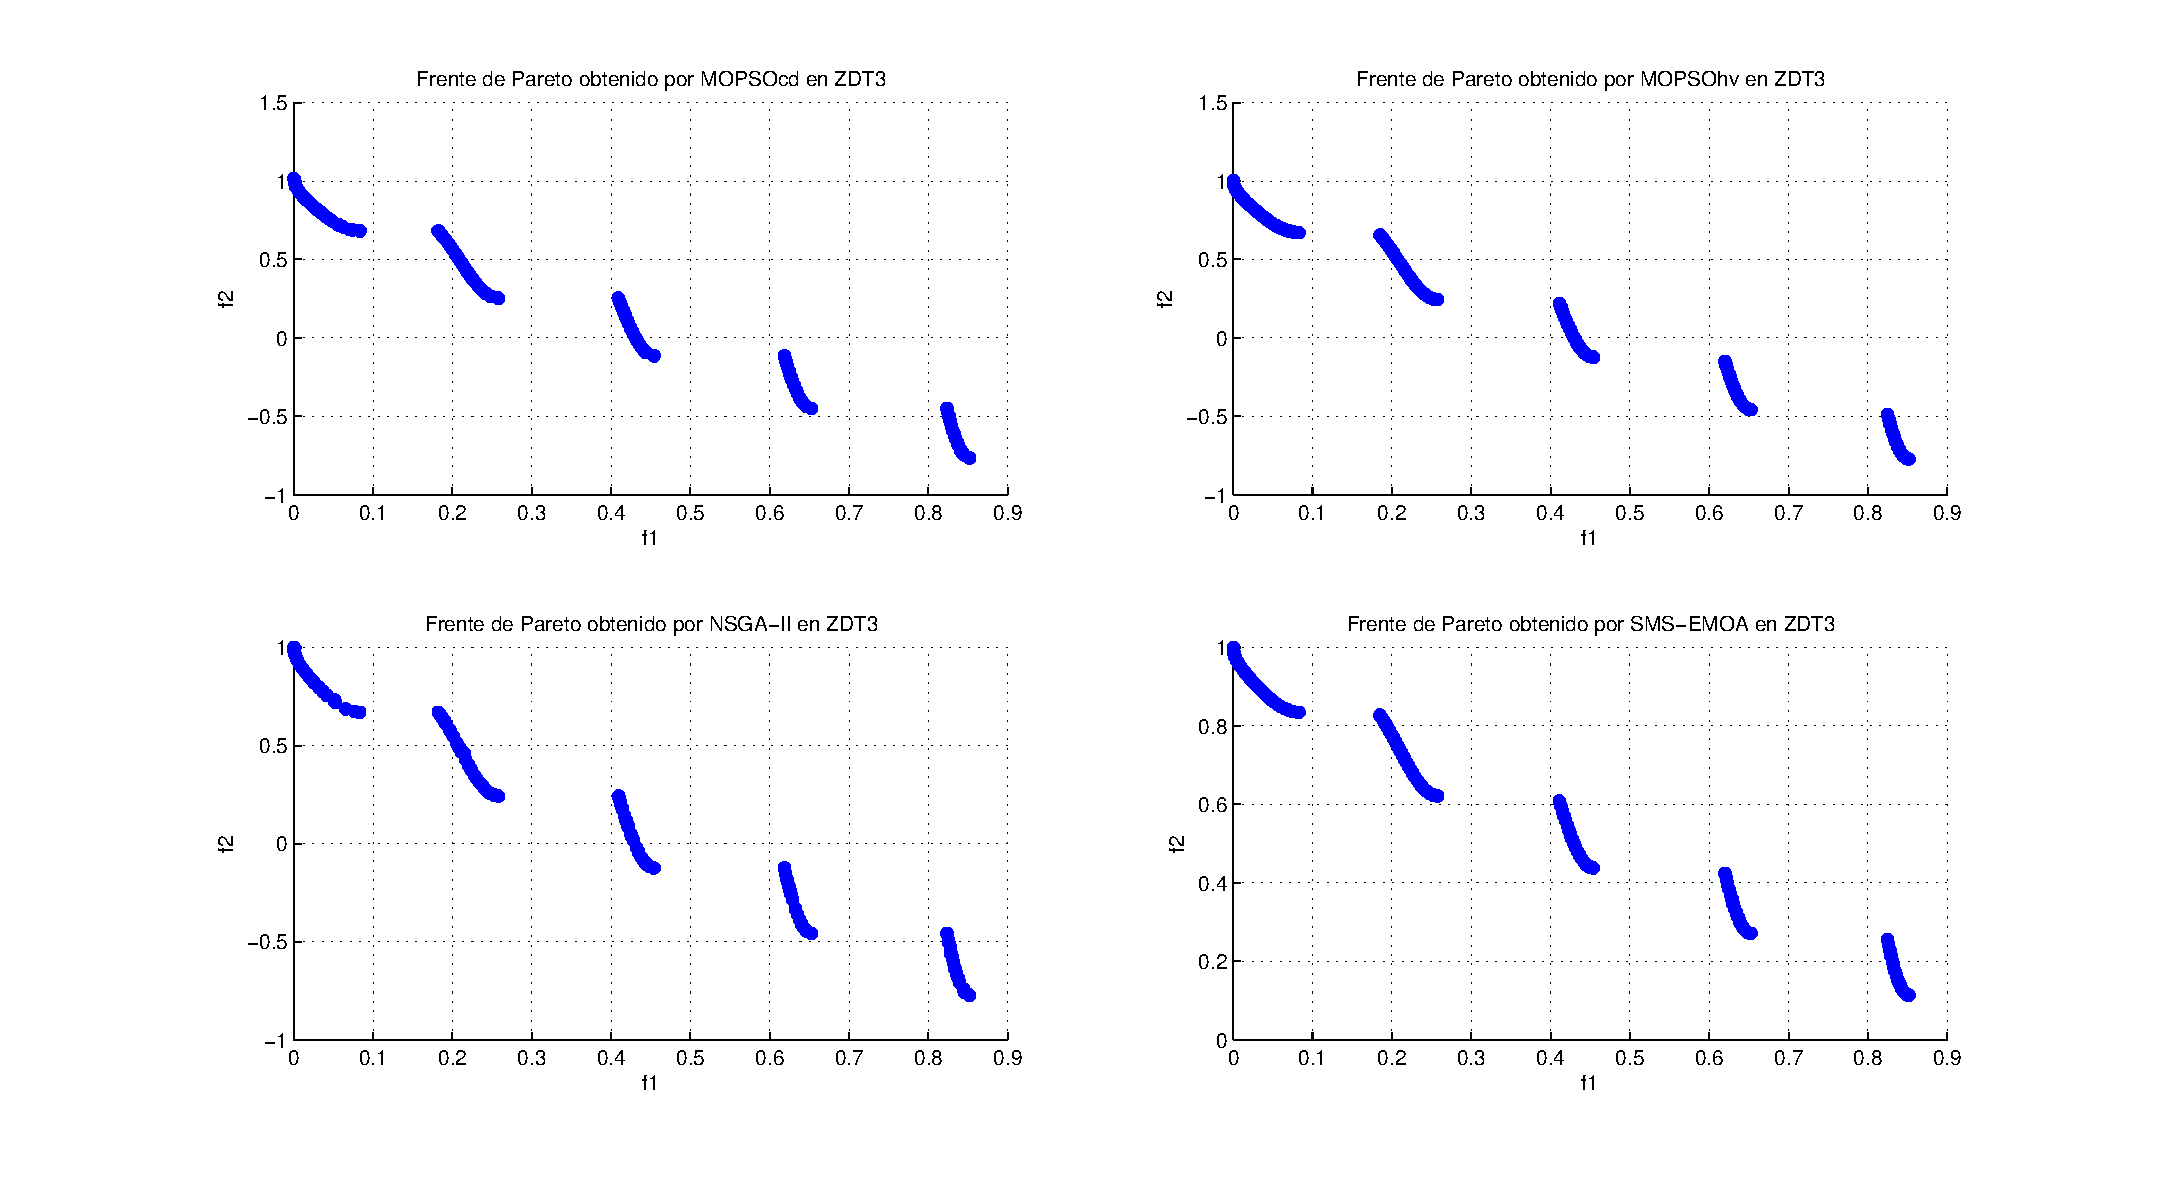
\includegraphics[scale=0.45]{Cap4/rzdt3r.eps}
      \end{center}
	\caption{Resultados gr\'aficos correspondientes al problema ZDT3.}
      \label{fig:rZDT3}
      \end{figure}
\clearpage
\newpage
 \begin{table}
 \begin{center}
  \begin{tabular}{|l|cc|cc|} \hline
    & \multicolumn{4}{|c|}{\textbf{Espaciado}} \\ 
	\textbf{Algoritmo} & \textbf{Menor} & \textbf{Mayor} & \textbf{Promedio} & \textbf{Desviaci\'on} \\  \hline\hline
	\textbf{MOPSOhv} &0.004345 & 0.005129 &\textbf{\textcolor{blue}{ 0.004679}}  &\textbf{ 0.000217} \\ 
	\textbf{MOPSOcd} &0.006054 & 0.007826 &\textbf{\textcolor{green}{ 0.007014}} &\textbf{\textcolor{green}{ 0.000517}}  \\ 
	\textbf{NSGA-II} &0.007089 & 0.009201 &\textbf{\textcolor{red}{ 0.008052}}   &\textbf{\textcolor{red}{ 0.000616}}  \\  
	\textbf{SMS-EMOA}&0.002105 & 0.002981 & \textbf{0.002492} &\textbf{\textcolor{blue}{ 0.000240}}\\  
	\hline\hline
    & \multicolumn{4}{|c|}{\textbf{DGI}} \\ 	\hline \hline
	\textbf{MOPSOhv} &0.027389 & 0.027394 & \textbf{\textcolor{green}{0.027391}} &\textbf{0.000001}   \\ 
	\textbf{MOPSOcd} &0.027462 & 0.027521 & \textbf{\textcolor{red}{0.027497}} & \textbf{\textcolor{red}{0.000015}}  \\ 
	\textbf{NSGA-II} &0.017008 & 0.017016 & \textbf{0.017011} & \textbf{\textcolor{blue}{0.000002}}   \\  
	\textbf{SMS-EMOA}&0.017008 & 0.017030 & \textbf{\textcolor{blue}{0.017011}} & \textbf{\textcolor{green}{0.000004}}  \\  
	\hline\hline
    & \multicolumn{4}{|c|}{\textbf{Hipervolumen}} \\ 	\hline \hline
	\textbf{MOPSOhv} &0.328865 & 0.329046 & \textbf{\textcolor{green}{0.328971}} & \textbf{0.000052}  \\ 
	\textbf{MOPSOcd} &0.323038 & 0.325624 & \textbf{\textcolor{red}{0.324090}} & \textbf{\textcolor{red}{0.000668}}  \\ 
	\textbf{NSGA-II} &0.653158 & 0.654108 & \textbf{\textcolor{blue}{0.653614}} & \textbf{\textcolor{green}{0.000237}}  \\  
	\textbf{SMS-EMOA}&0.654266 & 0.655054 & \textbf{0.654940} & \textbf{\textcolor{blue}{0.000165}}  \\  
	\hline
    & \multicolumn{4}{|c|}{\textbf{Cobertura}} \\ \hline\hline 
	\textbf{Algoritmo} & \textbf{MOPSOhv} & \textbf{MOPSOcd} & \textbf{NSGA-II} & \textbf{SMS-EMOA} \\  \hline \hline
	\textbf{MOPSOhv} & ---      & \textbf{1.000000} & \textbf{0.022500} & \textbf{0.033000} \\ 
	\textbf{MOPSOcd} & 0.000500 & ---      & 0.000001 & 0.000001   \\ 
	\textbf{NSGA-II} & 0.004000 & 1.000000 & ---      & 0.024500 \\  
	\textbf{SMS-EMOA}& 0.000001 & 0.991000 & 0.001000 & --- \\  
	\hline\hline
	\end{tabular}
\caption{Resultados del problema ZDT4.}
  \label{tab:zdt4}
\end{center}
\end{table}

La multimodalidad de ZDT4 causa dificultad a nuestra propuesta (MOPSOhv) para converger de manera \'optima, como se muestra en la 
tabla \ref{tab:zdt4}. Sin embargo, presenta una buena distribuci\'on de las soluciones quedando despu\'es del SMS-EMOA. Nuestra propuesta 
es superada por el SMS-EMOA y NSGA-II y conforme a estos resultados se puede crear una
jerarqu\'ia en orden descendente en t\'erminos de convergencia del conjunto de soluciones pr\'oximas al frente de Pareto real:

\begin{enumerate}
  \item NSGA-II
  \item SMS-EMOA
  \item MOPSOhv
  \item MOPSOcd
\end{enumerate}

Tambi\'en, se observa que en las soluciones de nuestra propuesta dominan a las soluciones de los otros algoritmos.

 \clearpage
 \newpage
 \begin{figure}
      \begin{center}
	  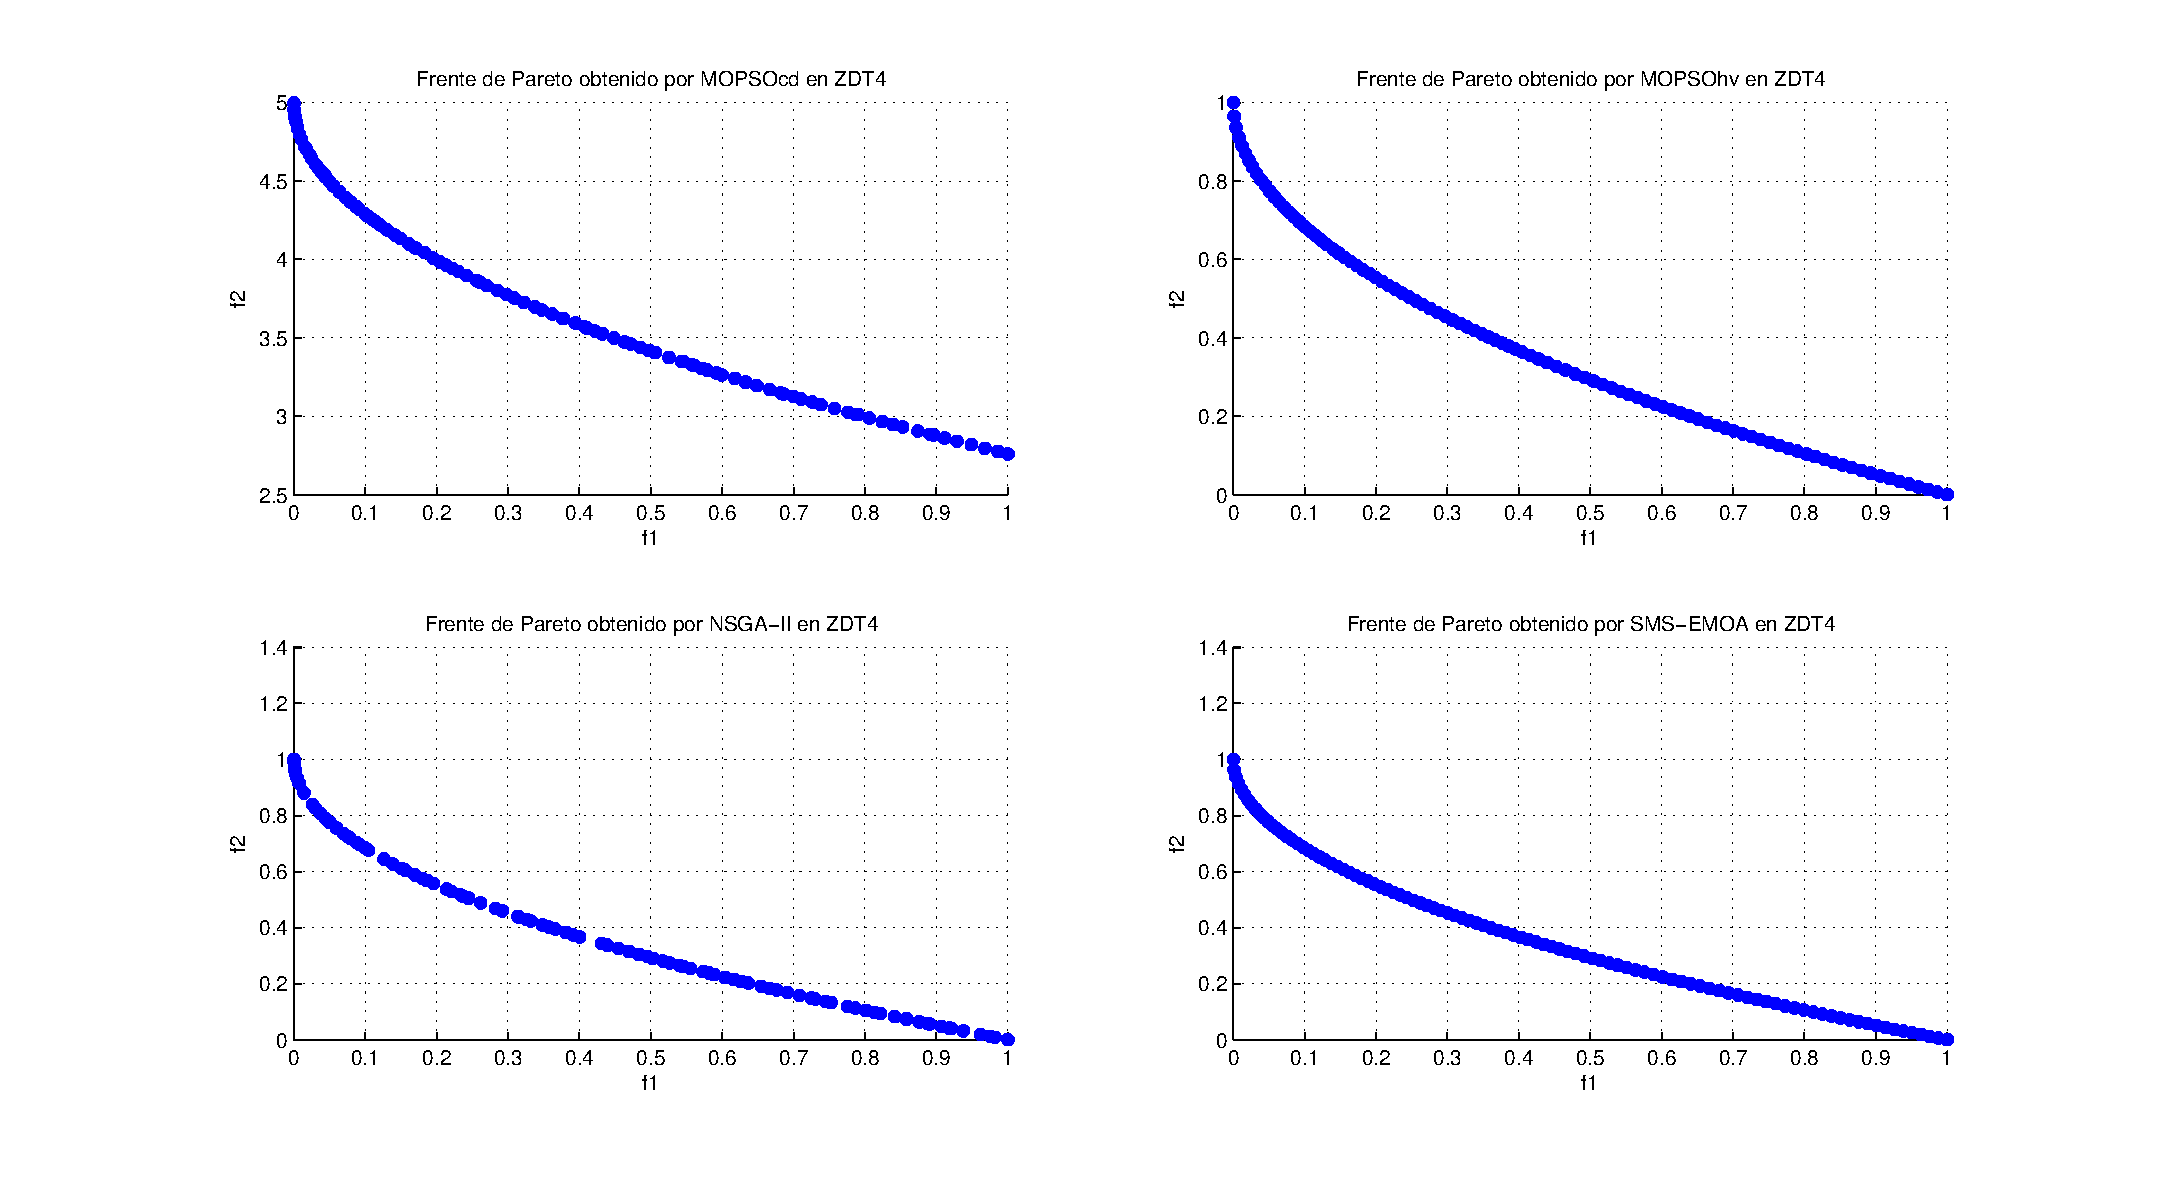
\includegraphics[scale=0.45]{Cap4/rzdt4r.eps}
      \end{center}
	\caption{Resultados gr\'aficos correspondientes al problema ZDT4.}
      \label{fig:rZDT4}
      \end{figure}
 \clearpage
 \newpage
 \begin{table}
 \begin{center}
  \begin{tabular}{|l|cc|cc|} \hline
    & \multicolumn{4}{|c|}{\textbf{Espaciado}} \\ 
	\textbf{Algoritmo} & \textbf{Menor} & \textbf{Mayor} & \textbf{Promedio} & \textbf{Desviaci\'on} \\  \hline\hline
	\textbf{MOPSOhv} &0.001587 & 0.002728 & \textbf{\textcolor{blue}{ 0.001975}} & \textbf{\textcolor{blue}{0.000324}}  \\ 
	\textbf{MOPSOcd} &0.042774 & 0.294482 & \textbf{\textcolor{red}{0.115691}} & \textbf{\textcolor{red}{0.053160}} \\ 
	\textbf{NSGA-II} &0.005925 & 0.007914 & \textbf{\textcolor{green}{0.007055}} & \textbf{\textcolor{green}{0.000437 }} \\  
	\textbf{SMS-EMOA}&0.000256 & 0.001011 & \textbf{0.000603} & \textbf{0.000181} \\  
	\hline\hline
    & \multicolumn{4}{|c|}{\textbf{DGI}} \\ 	\hline \hline
	\textbf{MOPSOhv} &0.027380 & 0.027549 & \textbf{\textcolor{green}{0.027434}} & \textbf{\textcolor{green}{0.000046}}  \\ 
	\textbf{MOPSOcd} &0.000281 & 0.000281 & \textbf{0.000281} & \textbf{0.000000}  \\ 
	\textbf{NSGA-II} &0.017011 & 0.027398 & \textbf{\textcolor{red}{0.026356}} & \textbf{\textcolor{red}{0.003115}}  \\  
	\textbf{SMS-EMOA}&0.027390 & 0.027397 & \textbf{\textcolor{blue}{0.027395}} & \textbf{\textcolor{blue}{0.000002}}  \\  
	\hline\hline
    & \multicolumn{4}{|c|}{\textbf{Hipervolumen}} \\ \hline \hline
	\textbf{MOPSOhv} &0.496939 & 0.54493 & \textbf{\textcolor{blue}{0.512122}} & \textbf{\textcolor{blue}{0.002083}}  \\ 
	\textbf{MOPSOcd} &0.156527 & 0.479775 & \textbf{\textcolor{red}{0.383107}} & \textbf{\textcolor{green}{0.076527}} \\ 
	\textbf{NSGA-II} &0.480422 & 0.870700 & \textbf{0.519667} & \textbf{\textcolor{red}{0.117011}} \\  
	\textbf{SMS-EMOA}&0.503836 & 0.504173 & \textbf{\textcolor{green}{0.503956}} & \textbf{0.000093} \\  
	\hline\hline
    & \multicolumn{4}{|c|}{\textbf{Cobertura}} \\ \hline\hline 
	\textbf{Algoritmo} & \textbf{MOPSOhv} & \textbf{MOPSOcd} & \textbf{NSGA-II} & \textbf{SMS-EMOA} \\  \hline \hline
	\textbf{MOPSOhv} &---       & \textbf{0.127778} & \textbf{\textcolor{red}{0.000001}}  & \textbf{\textcolor{red}{0.000001}} \\ 
	\textbf{MOPSOcd} & 0.059000 & ---      & 0.025500  & 0.019000  \\ 
	\textbf{NSGA-II} & \textbf{0.037500} & 0.645500 & ---       & 0.011000 \\  
	\textbf{SMS-EMOA}& \textbf{0.138889} & 0.850000 & 0.009000  & --- \\  
	\hline
	\end{tabular}
\caption{Resultados correspondientes al problema ZDT6.}
  \label{tab:zdt6}
\end{center}
\end{table}

El espacio de los objetivos para ZDT6 muestra una densidad no uniforme causa dificultad a nuestra propuesta (MOPSOhv) para converger de manera \'optima, 
como se muestra en la tabla \ref{tab:zdt6}. Sin embargo, presenta una buena distribuci\'on de las soluciones quedando despu\'es del SMS-EMOA y 
superando al MOPSOcd, ya que este no es capaz de alcanzar una buena aproximaci\'on al frente de Pareto real. Nuestra propuesta es superada 
por el SMS-EMOA y NSGA-II y conforme a estos resultados se puede crear una
jerarqu\'ia en orden descendente en t\'erminos de convergencia del conjunto de soluciones pr\'oximas al frente de Pareto real:

\begin{enumerate}
  \item NSGA-II
  \item SMS-EMOA
  \item MOPSOhv
  \item MOPSOcd
\end{enumerate}

Tambi\'en, se observa que en las soluciones de nuestra propuesta dominan a las soluciones del MOPSOcd y siendo superado por las soluciones
de manera ligera por el NSGA-II y SMS-EMOA.

\clearpage
\newpage
%\begin{landscape}

  \begin{figure}
      \begin{center}
	  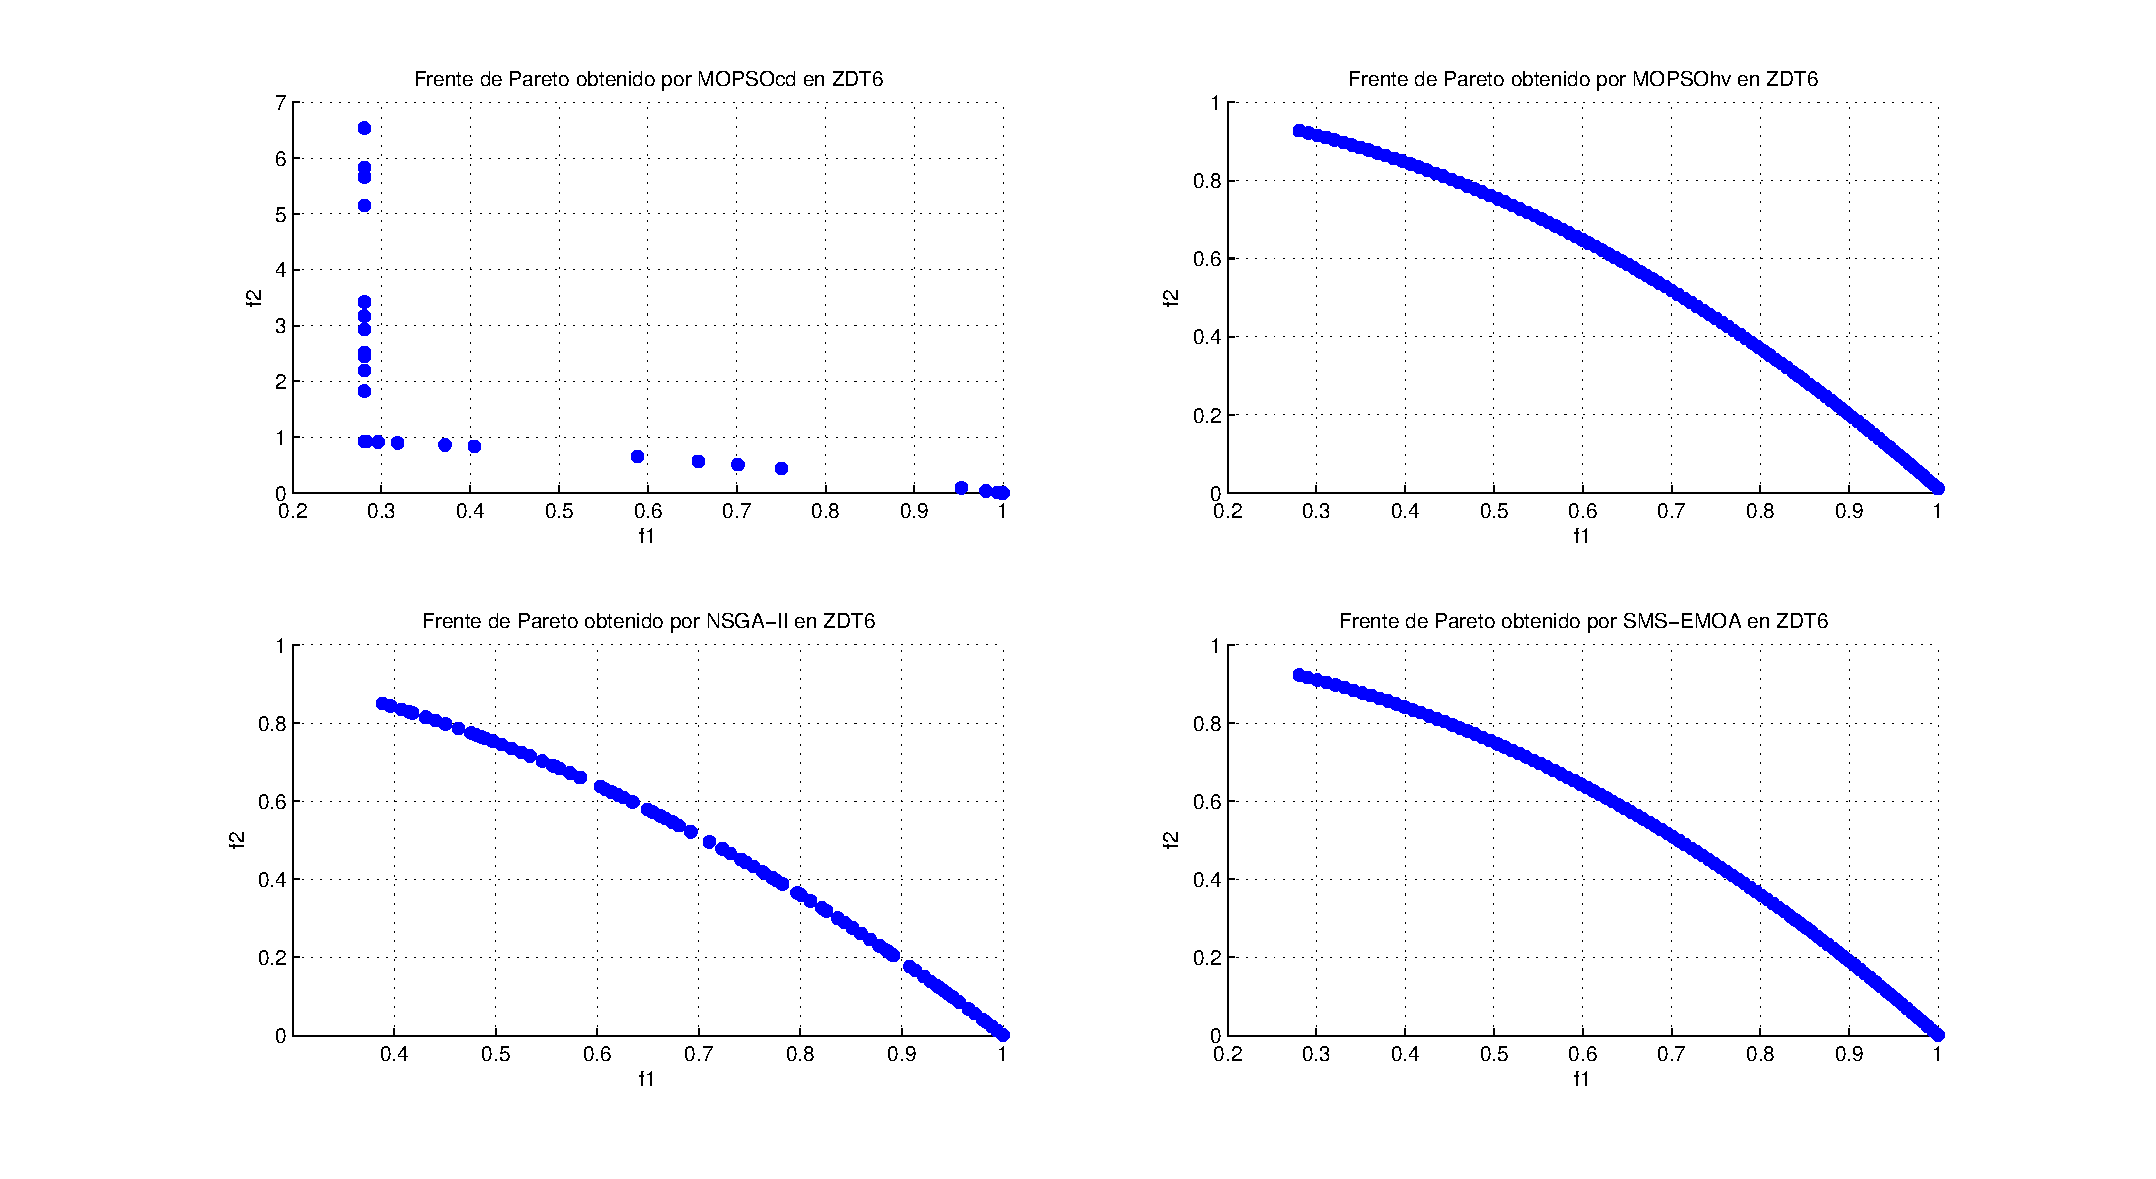
\includegraphics[scale=0.45]{Cap4/rzdt6r.eps}
      \end{center}
	\caption{Resultados gr\'aficos correspondientes al problema ZDT6.}
      \label{fig:rZDT6}
      \end{figure}
%\end{landscape}
\clearpage
   
  
\section{Conjunto de problemas DTLZ} 

Los problemas siguientes son parte de la serie de problemas DTLZ con tres funciones objetivo, tal y como se describen a continuaci\'on 
\cite{dtlz2002a}:

\begin{itemize}
\item La funci\'on de prueba \textbf{DTLZ1} tiene un frente de Pareto lineal, separable y multimodal:

\begin{align*}
f_1(x)&=\frac{1}{2}\cdot x_1\cdot x_2 \cdot \ldots \cdot x_{M-1} \cdot (1+g(x))\\
f_2(x)&=\frac{1}{2}\cdot x_1\cdot x_2 \cdot \ldots \cdot(1-x_{M-1})\cdot(1+g(x))\\
\vdots&\\
f_M(x)&=\frac{1}{2}\cdot(1-x_1)\cdot(1+g(x))\\
g(x)&=100\cdot[k+\sum_{i=M}^n(x_i-0.5)^2-cos(20\cdot\pi\cdot(x_i-0.5))]
\end{align*}

donde $n=M+k-1$ (se sugiere una $k=5$) y $x_i\in[0,1]$ con $i = 1, \ldots, n$ (figura \ref{fig:dtlz1}).


 \item La funci\'on de prueba \textbf{DTLZ2} tiene un frente de Pareto c\'oncavo:
\begin{align*}
f_1(x)&=\cos(x_1\frac{\pi}{2})\cdot\cos(x_2\frac{\pi}{2})\cdot\ldots\cdot\cos(x_{M-1}\frac{\pi}{2})\cdot(1+g(x))\\
f_2(x)&=\cos(x_1\frac{\pi}{2})\cdot\cos(x_2\frac{\pi}{2})\cdot\ldots\cdot\sin(x_{M-1}\frac{\pi}{2})\cdot(1+g(x))\\
f_3(x)&=\cos(x_1\frac{\pi}{2})\cdot\cos(x_2\frac{\pi}{2})\cdot\ldots\cdot\sin(x_{M-2}\frac{\pi}{2})\cdot(1+g(x))\\
\vdots&\\
f_{M-1}(x)&=\cos(x_1\frac{\pi}{2})\cdot\sin(x_2\frac{\pi}{2})(1+g(x))\\
f_{M}(x)&=\sin(x_1\frac{\pi}{2})\cdot(1+g(x))\\
g(x)&=\sum_i=(x_i-0.5)^2
\end{align*}

donde $n=M+k-1$ (se sugiere una $k=10$) y $x_i\in[0,1]$ con $i= 1, \ldots, n$. Este problema se puede utilizar para investigar la 
escalabilidad (figura \ref{fig:dtlz2}).

\item La funci\'on de prueba \textbf{DTLZ3} tiene un frente de Pareto c\'oncavo y multimodal:
\begin{align*}
f_1(x)&=\cos(x_1\frac{\pi}{2})\cdot\cos(x_2\frac{\pi}{2})\cdot\ldots\cdot \cos(x_{M-1}\frac{\pi}{2})\cdot(1+g(x))\\
f_2(x)&=\cos(x_1\frac{\pi}{2})\cdot\cos(x_2\frac{\pi}{2})\cdot\ldots\cdot \sin(x_{M-1}\frac{\pi}{2})\cdot(1+g(x))\\
f_3(x)&=\cos(x_1\frac{\pi}{2})\cdot\cos(x_2\frac{\pi}{2})\cdot\ldots\cdot \sin(x_{M-2}\frac{\pi}{2})\cdot(1+g(x))\\
\vdots&\\
f_{M-1}(x)&=\cos(x_1\frac{\pi}{2})\cdot\sin(x_2\frac{\pi}{2})\cdot(1+g(x))\\
f_{M}(x)&=\sin(x_1\frac{\pi}{2})\cdot (1+g(x))\\
g(x)&=100\cdot [k+\sum_{i=M}^n(x_i-0.5)^2-\cos(20\cdot\pi\cdot(x_i-0.5))]
\end{align*}

donde $n=M+k-1$ (se sugiere una $k=10$) y $x_i\in[0,1]$ con $i=1, \ldots, n$. La forma del frente de Pareto de este
problema es similar al del problema DTLZ2 (figura \ref{fig:dtlz2}).

\item La funci\'on de prueba \textbf{DTLZ4} tiene un frente de Pareto c\'oncavo, separable y multimodal:

\begin{align*}
f_1(x)&=\cos(x_1^\alpha\frac{\pi}{2})\cdot\cos(x_2^\alpha\frac{\pi}{2})\cdot\ldots\cdot \cos(x_{M-1}^\alpha\frac{\pi}{2})\cdot(1+g(x))\\
f_2(x)&=\cos(x_1^\alpha\frac{\pi}{2})\cdot\cos(x_2^\alpha\frac{\pi}{2})\cdot\ldots\cdot \sin(x_{M-1}^\alpha\frac{\pi}{2})\cdot(1+g(x))\\
f_3(x)&=\cos(x_1^\alpha\frac{\pi}{2})\cdot\cos(x_2^\alpha\frac{\pi}{2})\cdot\ldots\cdot \sin(x_{M-2}^\alpha\frac{\pi}{2})\cdot(1+g(x))\\
\vdots&\\
f_{M-1}(x)&=\cos(x_1^\alpha\frac{\pi}{2})\cdot\sin(x_2^\alpha\frac{\pi}{2})\cdot(1+g(x))\\
f_{M}(x)&=\sin(x_1^\alpha\frac{\pi}{2})\cdot(1+g(x))\\
g(x)&=\sum_i(x_i-0.5)^2
\end{align*}

donde $n=M+k-1$ (se sugiere una $k=10$ y $\alpha=100$) y $x_i\in[0,1]$ con $i=1,\ldots, n$. Este problema prueba la habilidad de mantener 
una buena distribuci\'on de las soluciones. La forma del frente de Pareto de este
problema es similar al del problema DTLZ2 (figura \ref{fig:dtlz2}).

\item \textbf La funci\'on de prueba \textbf{DTLZ5} tiene un frente de Pareto curvo:

\begin{align*}
f_1(x)&=\cos(\theta_1\frac{\pi}{2})\cdot\cos(\theta_2\frac{\pi}{2})\cdot\ldots\cdot \cos(\theta_{M-1}\frac{\pi}{2})\cdot(1+g(x))\\
f_2(x)&=\cos(\theta_1\frac{\pi}{2})\cdot\cos(\theta_2\frac{\pi}{2})\cdot\ldots\cdot \sin(\theta_{M-1}\frac{\pi}{2})\cdot(1+g(x))\\
f_3(x)&=\cos(\theta_1\frac{\pi}{2})\cdot\cos(\theta_2\frac{\pi}{2})\cdot\ldots\cdot \sin(\theta_{M-2}\frac{\pi}{2})\cdot(1+g(x))\\
\vdots&\\
f_{M-1}(x)&=\cos(\theta_1\frac{\pi}{2})\cdot\sin(\theta_2\frac{\pi}{2})\cdot(1+g(x))\\
f_{M}(x)&=\sin(\theta_1\frac{\pi}{2})\cdot(1+g(x))\\
\theta_1&=\frac{\pi}{2}x_1\\
\theta_i&=\frac{\pi}{4\cdot(1+g(x))}(1+2\cdot g(x)\cdot x_i),  \text{para} \hspace{1mm} i=2,3\dots,(M-1)\\
g(x)&=\sum^n_i(x_i-0.5)^2
\end{align*}

donde $n=M+k-1$ (se sugiere una $k=10$) y $x_i\in[0,1]$ con $i = 1,\ldots,n$ (figura \ref{fig:dtlz5}).

\item La funci\'on de prueba \textbf{DTLZ6} tiene un frente de Pareto curvo:

\begin{align*}
f_1(x)&=\cos(\theta_1\frac{\pi}{2})\cdot\cos(\theta_2\frac{\pi}{2})\cdot\ldots\cdot \cos(\theta_{M-1}\frac{\pi}{2})\cdot(1+g(x))\\
f_2(x)&=\cos(\theta_1\frac{\pi}{2})\cdot\cos(\theta_2\frac{\pi}{2})\cdot\ldots\cdot \sin(\theta_{M-1}\frac{\pi}{2})\cdot(1+g(x))\\
f_3(x)&=\cos(\theta_1\frac{\pi}{2})\cdot\cos(\theta_2\frac{\pi}{2})\cdot\ldots\cdot \sin(\theta_{M-2}\frac{\pi}{2})\cdot(1+g(x))\\
\vdots&\\
f_{M-1}(x)&=\cos(\theta_1\frac{\pi}{2})\cdot\sin(\theta_2\frac{\pi}{2})\cdot(1+g(x))\\
f_{M}(x)&=\sin(\theta_1\frac{\pi}{2})\cdot(1+g(x))\\
\theta_1&=\frac{\pi}{2}x_1\\
\theta_i&=\frac{\pi}{4(1+g(x))}(1+2\cdot g(x)\cdot x_i),  \text{para}\hspace{1mm} i=2,3\dots,(M-1)\\
g(x)&=\sum^n_i=(x_i-0.5)^0.1
\end{align*}

donde $n=M+k-1$ (se sugiere una $k=10$) y $x_i\in[0,1]$ con $i=1,\ldots,n$ (figura \ref{fig:dtlz6}).

\item La funci\'on de prueba \textbf{DTLZ7} tiene un frente de Pareto discontinuo:

\begin{align*}
f_1(x)&=x_1 \\
f_2(x)&=x_2\\
\vdots&\\
f_{M-1}(x)&=x_{M-1}\\
f_{M}(x)&=(1+g(x_M))\cdot h(f_1,f_2,\dots,f_{M-1}g(x))\\
g(x)&=1+\frac{9}{k}\cdot\sum_{i=2}^nx_i\\
h(f_1,f_2,\dots,f_{M-1}g(x))&=M-\sum_{i=1}^{M-1}(\frac{f_i}{1+g(x)}(1+\sin{(3\cdot\pi\cdot f_i)}))
\end{align*}

donde $n=M+k-1$ (se sugiere una $k=20$) y $x_i\in[0,1]$ con $i=1,\ldots,n$. Este problema prueba la habilidad de mantener 
individuos en las diferentes regiones del frente de Pareto (figura \ref{fig:dtlz7}).

\end{itemize}


\begin{figure}
    \centering
    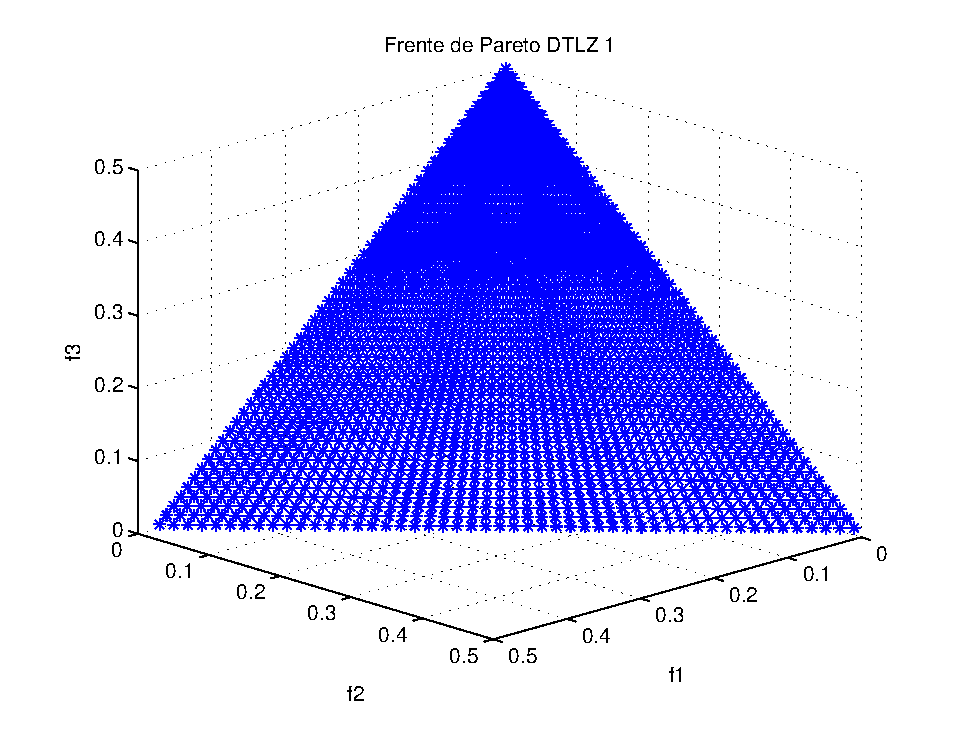
\includegraphics[scale=0.7]{ApendiceA/paretoDTLZ1.eps}
    \caption{Frente de Pareto verdadero de DTLZ1}
    \label{fig:dtlz1}
\end{figure}

\begin{figure}
    \centering
    \includegraphics[scale=0.7]{ApendiceA/paretoDTLZ2.eps}
    \caption{Frente de Pareto verdadero de DTLZ2}
    \label{fig:dtlz2}
\end{figure}
2\begin{figure}
    \centering
    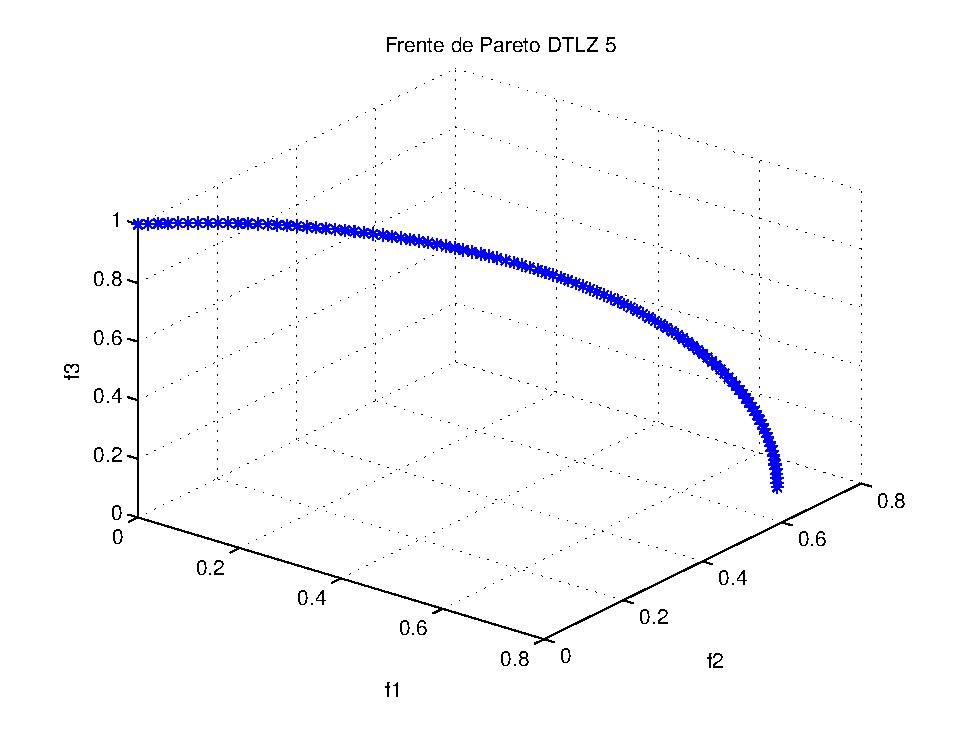
\includegraphics[scale=0.7]{ApendiceA/paretoDTLZ5.eps}
    \caption{Frente de Pareto verdadero de DTLZ5}
    \label{fig:dtlz5}
\end{figure}
\begin{figure}
  \centering
    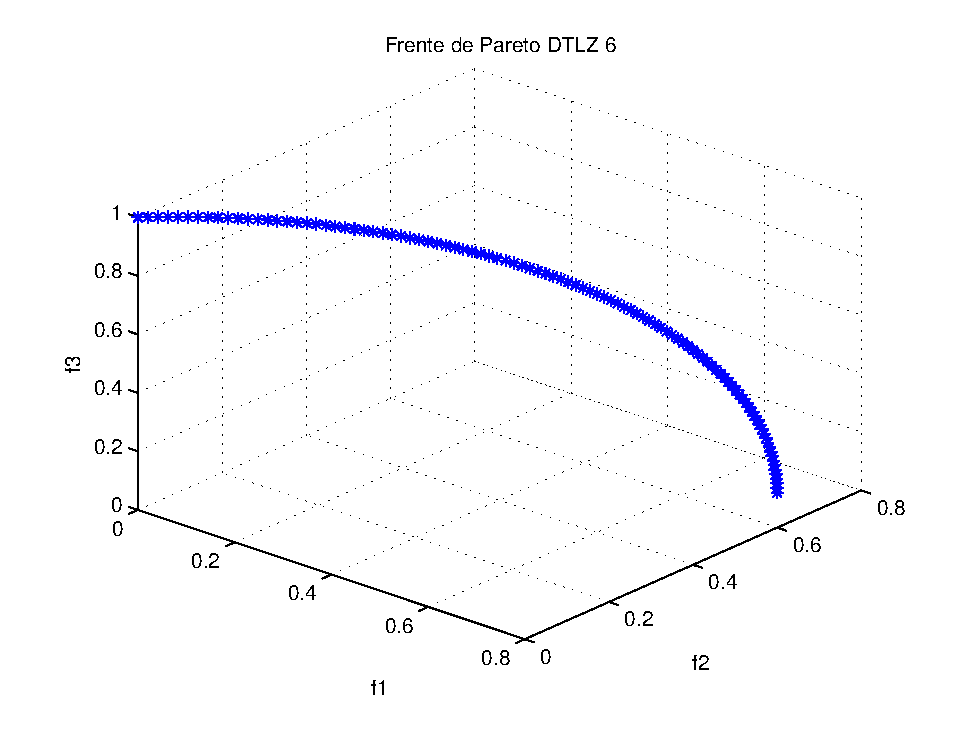
\includegraphics[scale=0.7]{ApendiceA/paretoDTLZ6.eps}
    \caption{Frente de Pareto verdadero de DTLZ6}
   \label{fig:dtlz6}
\end{figure}
\begin{figure}
 \centering
    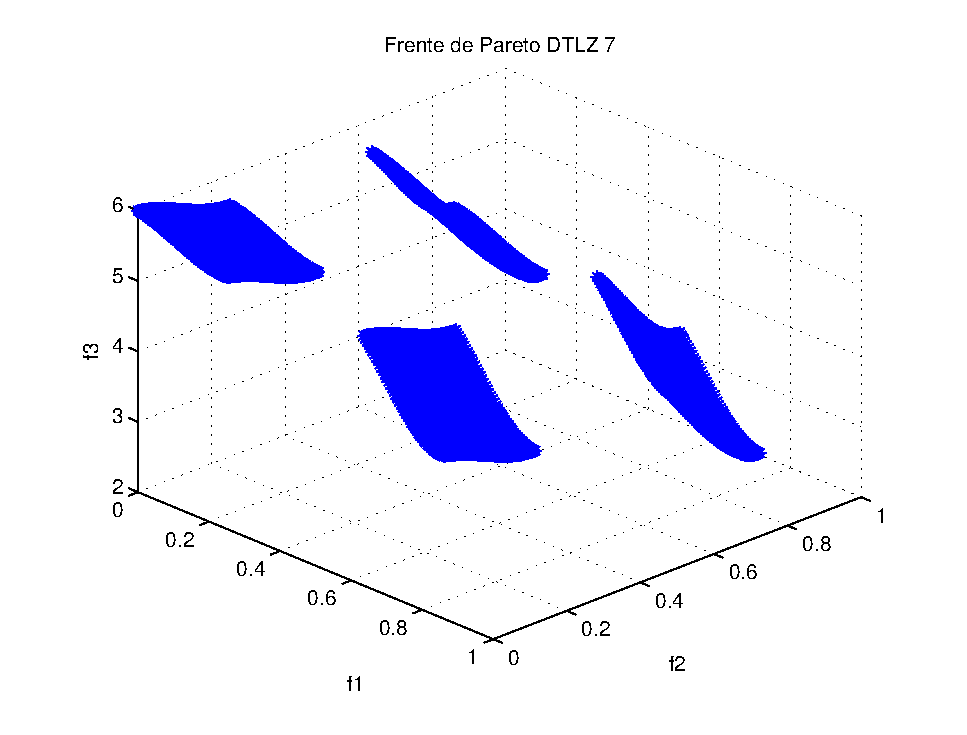
\includegraphics[scale=0.7]{ApendiceA/paretoDTLZ7.eps}
    \caption{Frente de Pareto verdadero de DTLZ7}
    \label{fig:dtlz7}
\end{figure}

\newpage

\section{Evaluaci\'on del conjunto de problemas DTLZ}

Para calcular la m\'etrica del hipervolumen se utiliza como punto de referencia el mostrado en la tabla \ref{tab:refdtlz}.

Los resultados obtenidos por nuestra propuesta (MOPSOhv) para los problemas DTLZ1, DTLZ3 y DTLZ6 son mejores que los obtenidos por el MOPSOcd,
ya que las soluciones de nuestra propuesta, seg\'un la m\'etrcia de cobertura, dominan completamente las soluciones arrojadas por MOPSOcd. 
Sin embargo, los resultados de nuestra propuesta son malos en comparaci\'on con los obtenidos por SMS-EMOA y NSGA-II, los cuales 
obtuvieron soluciones que dominan completamente a las nuestras como se muestra en las tablas \ref{tab:dtlz1}, \ref{tab:dtlz3} y \ref{tab:dtlz6}. 

  Conforme a estos resultados se tiene una jerarqu\'ia en orden descendente en t\'erminos de convergencia en estos primeros tres 
  problemas:

\begin{enumerate}
  \item NSGA-II
  \item SMS-EMOA
  \item MOPSOhv
  \item MOPSOcd
\end{enumerate}

El problema DTLZ4 presenta un frente de Pareto c\'oncavo. En la la figura \ref{fig:rDTLZ4} se muestran como los 
resultados obtenidos por nuestra propuesta (MOPSOhv) se distribuyen hacia los extremos del frente de Pareto, lo que causa tener una menor 
cobertura sobre \'este y causando que el valor en 
la m\'etrica del hipervolumen sea menor que los otros algoritmos. Sin embargo, las soluciones dominan a las soluciones de los 
dem\'as algoritmos como se muestra en la tabla \ref{tab:dtlz4}.

El problema DTLZ5 presenta un frente de Pareto curvo. DTLZ5 se considera un problema f\'acil, ya que su espacio de b\'usqueda 
presenta sesgo hacia soluciones cercanas al frente de Pareto verdadero. La figura \ref{fig:rDTLZ5} muestra que los resultados son similares 
para todos los algoritmos. Sin embargo, nuestras soluciones (MOPSOhv) dominan a las soluciones de los dem\'as algoritmos
excepto por las de SMS-EMOA como se muestra en la tabla \ref{tab:dtlz5}.

El problema DTLZ7 presenta un frente de Pareto con regiones discontinuas. Los resultados de nuestra propuesta (MOPSOhv) son similares que los de 
los algoritmos NSGA-II y MOPSOcd. Sin embargo, nuestras soluciones son dominadas por las obtenidas por SMS-EMOA
(tabla \ref{tab:dtlz7}). La figura \ref{fig:rDTLZ7} muestra como las soluciones se concentran en una parte del frente de Pareto.

 Conforme a estos resultados se tiene una jerarqu\'ia general en orden descendente en t\'erminos de convergencia para  
 DTLZ4, DTLZ5 y DTLZ7 problemas:

\begin{enumerate}
  \item  NSGA-II
  \item SMS-EMOA
  \item MOPSOhv
  \item MOPSOcd
\end{enumerate}

\begin{table}
  \begin{center}
    \begin{tabular}{|l||c|}
	\hline
	Problema  & Punto de referencia \\ 
	\hline
	\hline
	DTLZ1 & $(1.1,1.1,1.1)$ \\ 
	\hline
	DTLZ2 &  $(1.1,1.1,1.1)$\\
	\hline
	DTLZ3 &  $(5.0,5.0,5.0)$\\
	\hline
	DTLZ4 &  $(1.1,1.1,1.1)$\\
	\hline
	DTLZ5 &  $(1.1,1.1,1.1)$\\
	\hline
	DTLZ6 &  $(1.1,1.1,1.1)$\\
	\hline
	DTLZ7 &  $(1.1,1.1,7.0)$\\
	\hline
  \end{tabular}
  \caption{Puntos de referencia utilizados para el conjunto de problemas DTLZ}
  \label{tab:refdtlz}
\end{center}
\end{table}
\clearpage
\newpage
\begin{table}
 \begin{center}
  \begin{tabular}{|l|cc|cc|} \hline
    & \multicolumn{4}{|c|}{Espaciado} \\ 
	\textbf{Algoritmo} & \textbf{Menor} & \textbf{Mayor} & \textbf{Promedio} & \textbf{Desviaci\'on} \\  \hline \hline
	MOPSOhv &0.026239 & 0.184637 &  \textbf{\textcolor{green}{0.081790}} &  \textbf{\textcolor{green}{0.045829}}    \\ 
	MOPSOcd &0.531066 & 1.547502 &  \textbf{\textcolor{red}{0.974734}} &  \textbf{\textcolor{red}{0.295577}}   \\ 
	NSGA-II &0.015203 & 0.023959 &  \textbf{\textcolor{blue}{0.019360}} & \textbf{\textcolor{blue}{ 0.002384  }} \\  
	SMS-EMOA&0.005793 & 0.012914 & \textbf{0.006947} &  \textbf{0.001461}   \\  
	\hline\hline
    & \multicolumn{4}{|c|}{DGI} \\ \hline\hline
	MOPSOhv &0.000617 & 0.035965 &  \textbf{\textcolor{green}{0.013359}} &  \textbf{\textcolor{green}{0.011381}}  \\ 
	MOPSOcd &0.145461 & 0.462595 &  \textbf{\textcolor{red}{0.269641}} &  \textbf{\textcolor{red}{0.080597}}  \\ 
	NSGA-II &0.000540 & 0.003699 & \textbf{0.001261} &  \textbf{\textcolor{red}{0.001148}}   \\  
	SMS-EMOA &0.005777 & 0.011575 &  \textbf{\textcolor{blue}{0.006088}} &  \textbf{\textcolor{blue}{0.001259}}  \\  
	\hline\hline
    & \multicolumn{4}{|c|}{Hipervolumen} \\ 
  \hline\hline
	MOPSOhv &0.000000 & 1.290672 &  \textbf{\textcolor{green}{0.838140}} & \textbf{\textcolor{green}{0.351522}}  \\ 
	MOPSOcd &0.000000 & 0.000000 &  \textbf{\textcolor{red}{0.000000}} &  \textbf{\textcolor{red}{0.000000}}  \\ 
	NSGA-II &1.244198 & 1.297406 &  \textbf{\textcolor{blue}{1.270538}} &  \textbf{0.016839}  \\  
	SMS-EMOA &1.123310 & 1.305100 &\textbf{ 1.295857} &  \textbf{\textcolor{blue}{0.039586}}  \\  
	\hline\hline
	& \multicolumn{4}{|c|}{\textbf{Cobertura}} \\ \hline\hline 
	\textbf{Algoritmo} & \textbf{MOPSOhv} & \textbf{MOPSOcd} & \textbf{NSGA-II} & \textbf{SMS-EMOA} \\  \hline \hline
	\textbf{MOPSOhv} & ---      & \textbf{0.964500} &  \textbf{\textcolor{red}{0.000000}} &  \textbf{\textcolor{red}{0.000000}}  \\ 
	\textbf{MOPSOcd} & 0.000000 & ---      &  0.000000  & 0.000000 \\ 
	\textbf{NSGA-II} & \textbf{0.838500} & 0.977500 & ---       & 0.039000 \\  
	\textbf{SMS-EMOA}& \textbf{0.771000} & 0.911500 & 0.000000  & --- \\  
	\hline
	\end{tabular}
\caption{Resultados correspondientes al problema DTLZ1.}
  \label{tab:dtlz1}
\end{center}
\end{table}
La multimodalidad de DTLZ1 causa dificultad a nuestra propuesta (MOSPSOhv) para converger de manera \'optima, como se muestra en la 
tabla \ref{tab:dtlz1}. En la gr\'afica \ref{fig:rDTLZ1} se muestra que el MOPSOcd no tiene una buena convergencia
al frente de Pareto y no muestra una buena distribuci\'on de las soluciones, por lo que nuestra propuesta se mantienen arriba de \'este.
Sin embargo, nuestra propuesta es superada por el SMS-EMOA y NSGA-II y conforme a estos resultados se puede crear una
jerarqu\'ia en orden descendente en t\'erminos de convergencia del conjunto de soluciones pr\'oximas al frente de Pareto real:

\begin{enumerate}
  \item NSGA-II
  \item SMS-EMOA
  \item MOPSOhv
  \item MOPSOcd
\end{enumerate}

\clearpage
\newpage

\begin{figure}
      \begin{center}
	  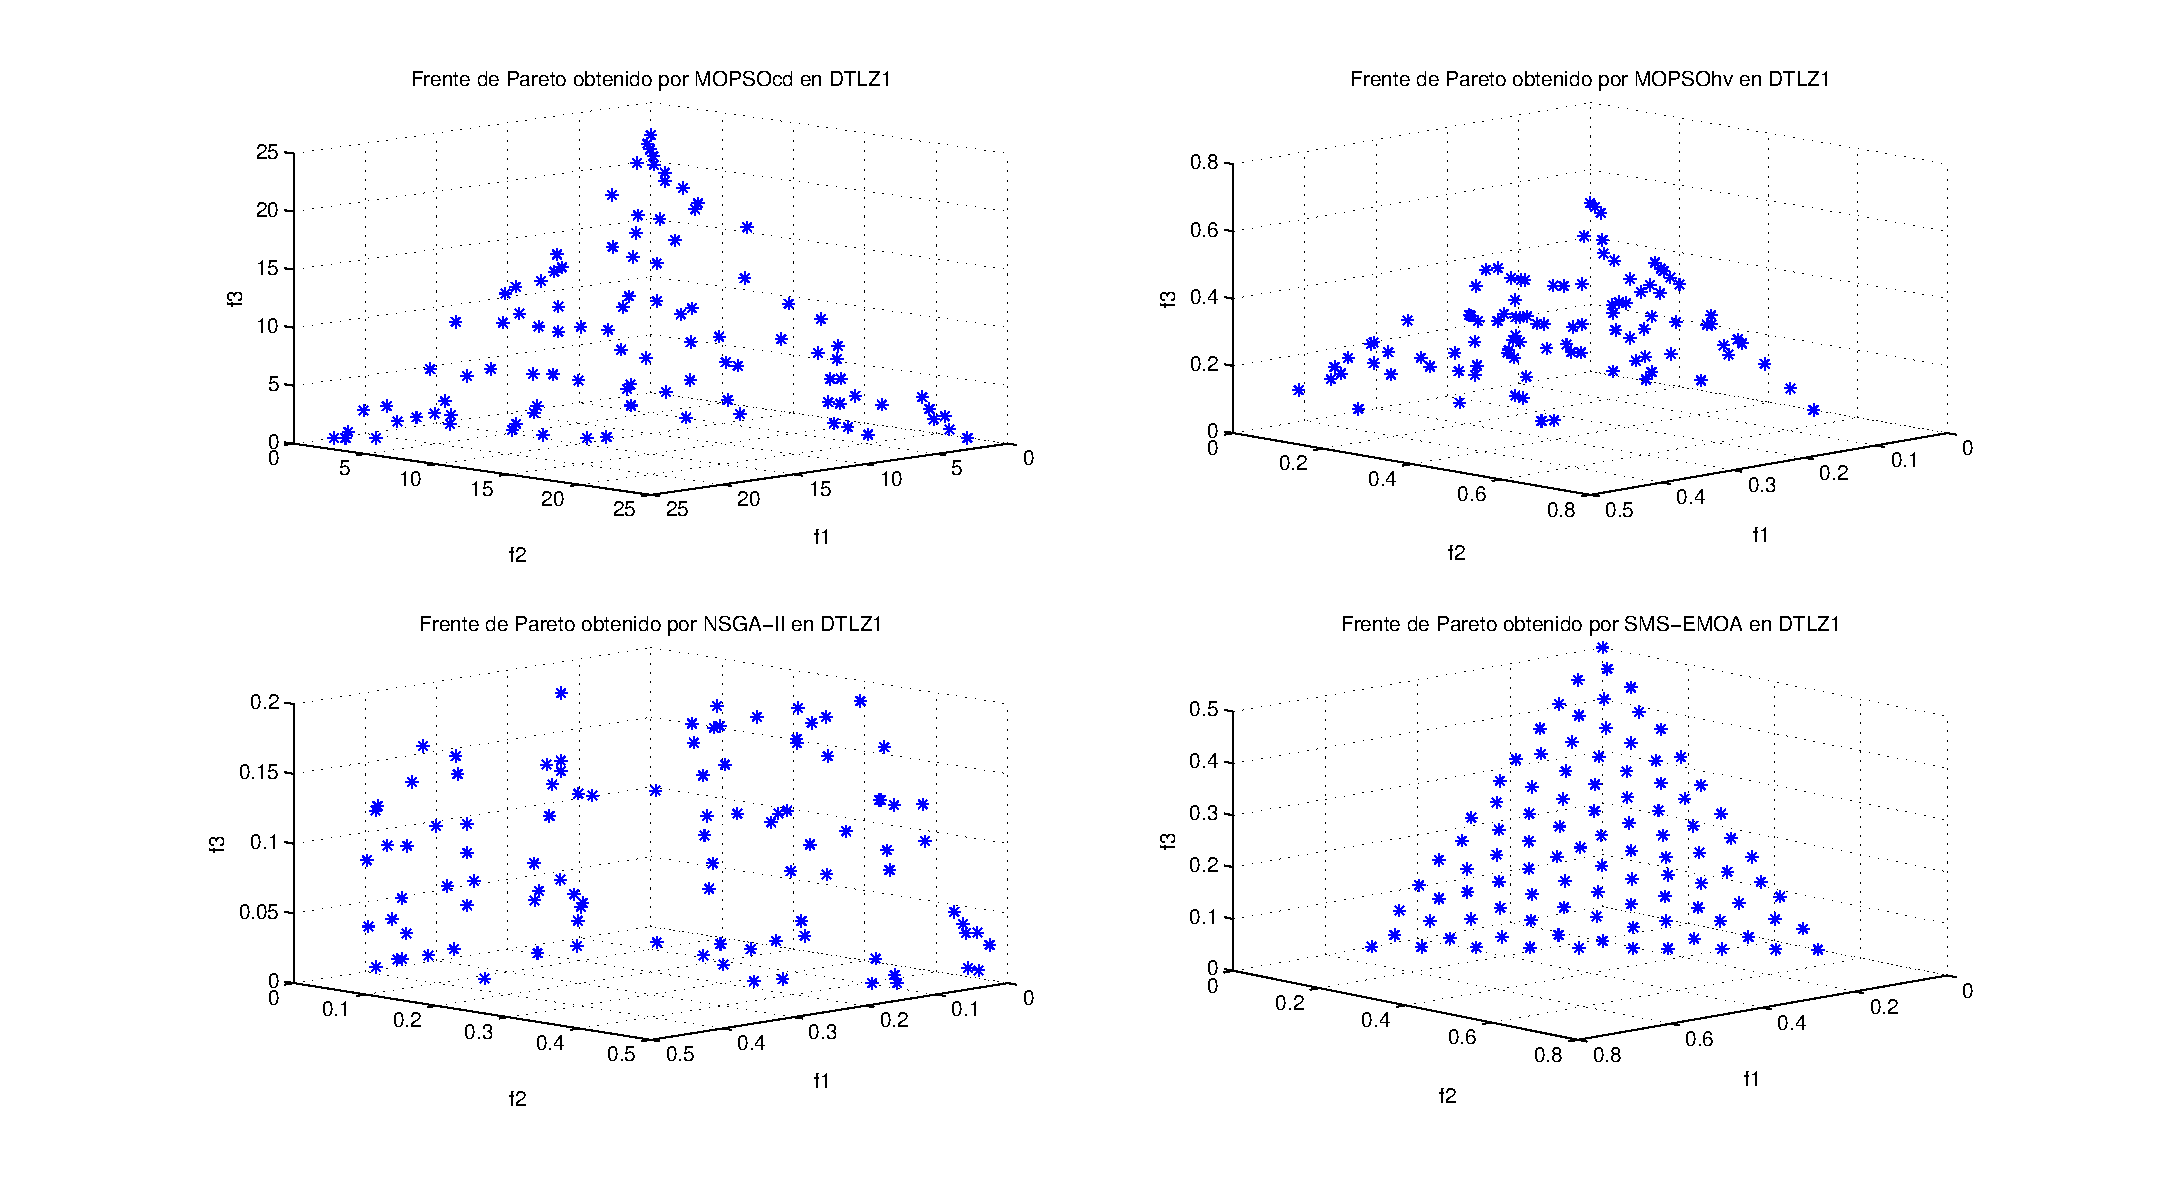
\includegraphics[scale=0.45]{Cap4/rdtlz1r.eps}
      \end{center}
	\caption{Resultados gr\'aficos correspondientes al problema DTLZ1.}
      \label{fig:rDTLZ1}
\end{figure}

\clearpage
\newpage

\begin{table}
 \begin{center}
  \begin{tabular}{|l|cc|cc|} \hline
    & \multicolumn{4}{|c|}{Espaciado} \\ 
	\textbf{Algoritmo} & \textbf{Menor} & \textbf{Mayor} & \textbf{Promedio} & \textbf{Desviaci\'on} \\  \hline \hline
	MOPSOhv &0.031912 & 0.087823 &  \textbf{\textcolor{red}{0.056173}} &  \textbf{\textcolor{red}{ 0.012780}}    \\ 
	MOPSOcd &0.042795 & 0.064965 &  \textbf{\textcolor{blue}{0.052077}} &  \textbf{\textcolor{green}{0.005154}}  \\ 
	NSGA-II &0.043968 & 0.065239 &  \textbf{\textcolor{green}{0.055460}} &  \textbf{\textcolor{blue}{0.005003}}   \\  
	SMS-EMOA &0.040210 & 0.047397 & \textbf{0.042716} &  \textbf{0.001942 }  \\  
	\hline\hline
    & \multicolumn{4}{|c|}{DGI} \\ 
	\hline\hline
	MOPSOhv &0.000421 & 0.003117 &  \textbf{\textcolor{green}{0.000806}} &  \textbf{\textcolor{green}{0.000611}}    \\ 
	MOPSOcd &0.000353 & 0.000430 & \textbf{0.000383} & \textbf{\textcolor{red}{ 0.000022}}   \\ 
	NSGA-II &0.000354 & 0.000437 &  \textbf{\textcolor{blue}{0.000380}} &  \textbf{\textcolor{blue}{0.000018}}   \\  
	SMS-EMOA &0.005000 & 0.005000 &  \textbf{\textcolor{red}{0.005000}} &  \textbf{0.000000}   \\  
	\hline\hline
    & \multicolumn{4}{|c|}{Hipervolumen} \\ 
	\hline \hline
	MOPSOhv &0.477781 & 0.695914 &  \textbf{\textcolor{red}{0.626972}} &  \textbf{\textcolor{red}{0.046583}}   \\ 
	MOPSOcd &0.637661 & 0.700693 &  \textbf{\textcolor{green}{0.669615}} &  \textbf{\textcolor{green}{0.019100}}   \\ 
	NSGA-II &0.676094 & 0.709199 &  \textbf{\textcolor{blue}{0.697212}} &  \textbf{\textcolor{blue}{0.007736}}   \\  
	SMS-EMOA &0.757997 & 0.758163 & \textbf{0.758091} &  \textbf{0.000047 }  \\  
	\hline\hline
	& \multicolumn{4}{|c|}{\textbf{Cobertura}} \\ \hline\hline 
	\textbf{Algoritmo} & \textbf{MOPSOhv} & \textbf{MOPSOcd} & \textbf{NSGA-II} & \textbf{SMS-EMOA} \\  \hline \hline
	\textbf{MOPSOhv} & ---       & \textbf{0.225500}  &  \textbf{0.009000} &  \textbf{\textcolor{red}{0.000000}} \\ 
	\textbf{MOPSOcd} &  0.000000 & ---       & 0.001500  & 0.000000  \\ 
	\textbf{NSGA-II} & 0.001000  &  0.296000 & ---       & 0.010000 \\  
	\textbf{SMS-EMOA}& \textbf{0.003000}  & 0.444000  &  0.006000 & --- \\  
	\hline
	\end{tabular}
\caption{Resultados correspondientes al problema DTLZ2.}
  \label{tab:dtlz2}
\end{center}
\end{table}

En el problema DTLZ2 se observa que en nuestra propuesta (MOPSOhv) no tiene una distribuci\'on de las soluciones, lo que causa que existan espacios grandes
en la aproximaci\'on al frente de Pareto, como se observa en la figura \ref{fig:rDTLZ2}, lo que causa que no se tenga una mayor cobertura 
del frente de Pareto, por lo tanto, el valor de la m\'etrica del hipervolumen disminuya, como se observa en la tabla \ref{tab:dtlz2}. Esto se 
debe, a que nuestra propuesta utiliza una m\'etrica que aproxima las contribuciones al hipervolumen para reemplazar soluciones en el archivo, 
por lo que, disminuye la calidad de las soluciones alcanzadas por \'este. Nuestra propuesta es superada por el SMS-EMOA y 
NSGA-II y conforme a estos resultados se puede crear una jerarqu\'ia en orden descendente en t\'erminos de convergencia del conjunto de 
soluciones pr\'oximas al frente de Pareto real:


\begin{enumerate}
  \item SMS-EMOA
  \item NSGA-II
  \item MOPSOhv
  \item MOPSOcd
\end{enumerate}

Tambi\'en, se observa que en las soluciones de nuestra propuesta dominan a las soluciones del NSGA-II y MOPSOcd, y siendo superado por las 
soluciones del SMS-EMOA.
\clearpage
\newpage

\begin{figure}
      \begin{center}
	  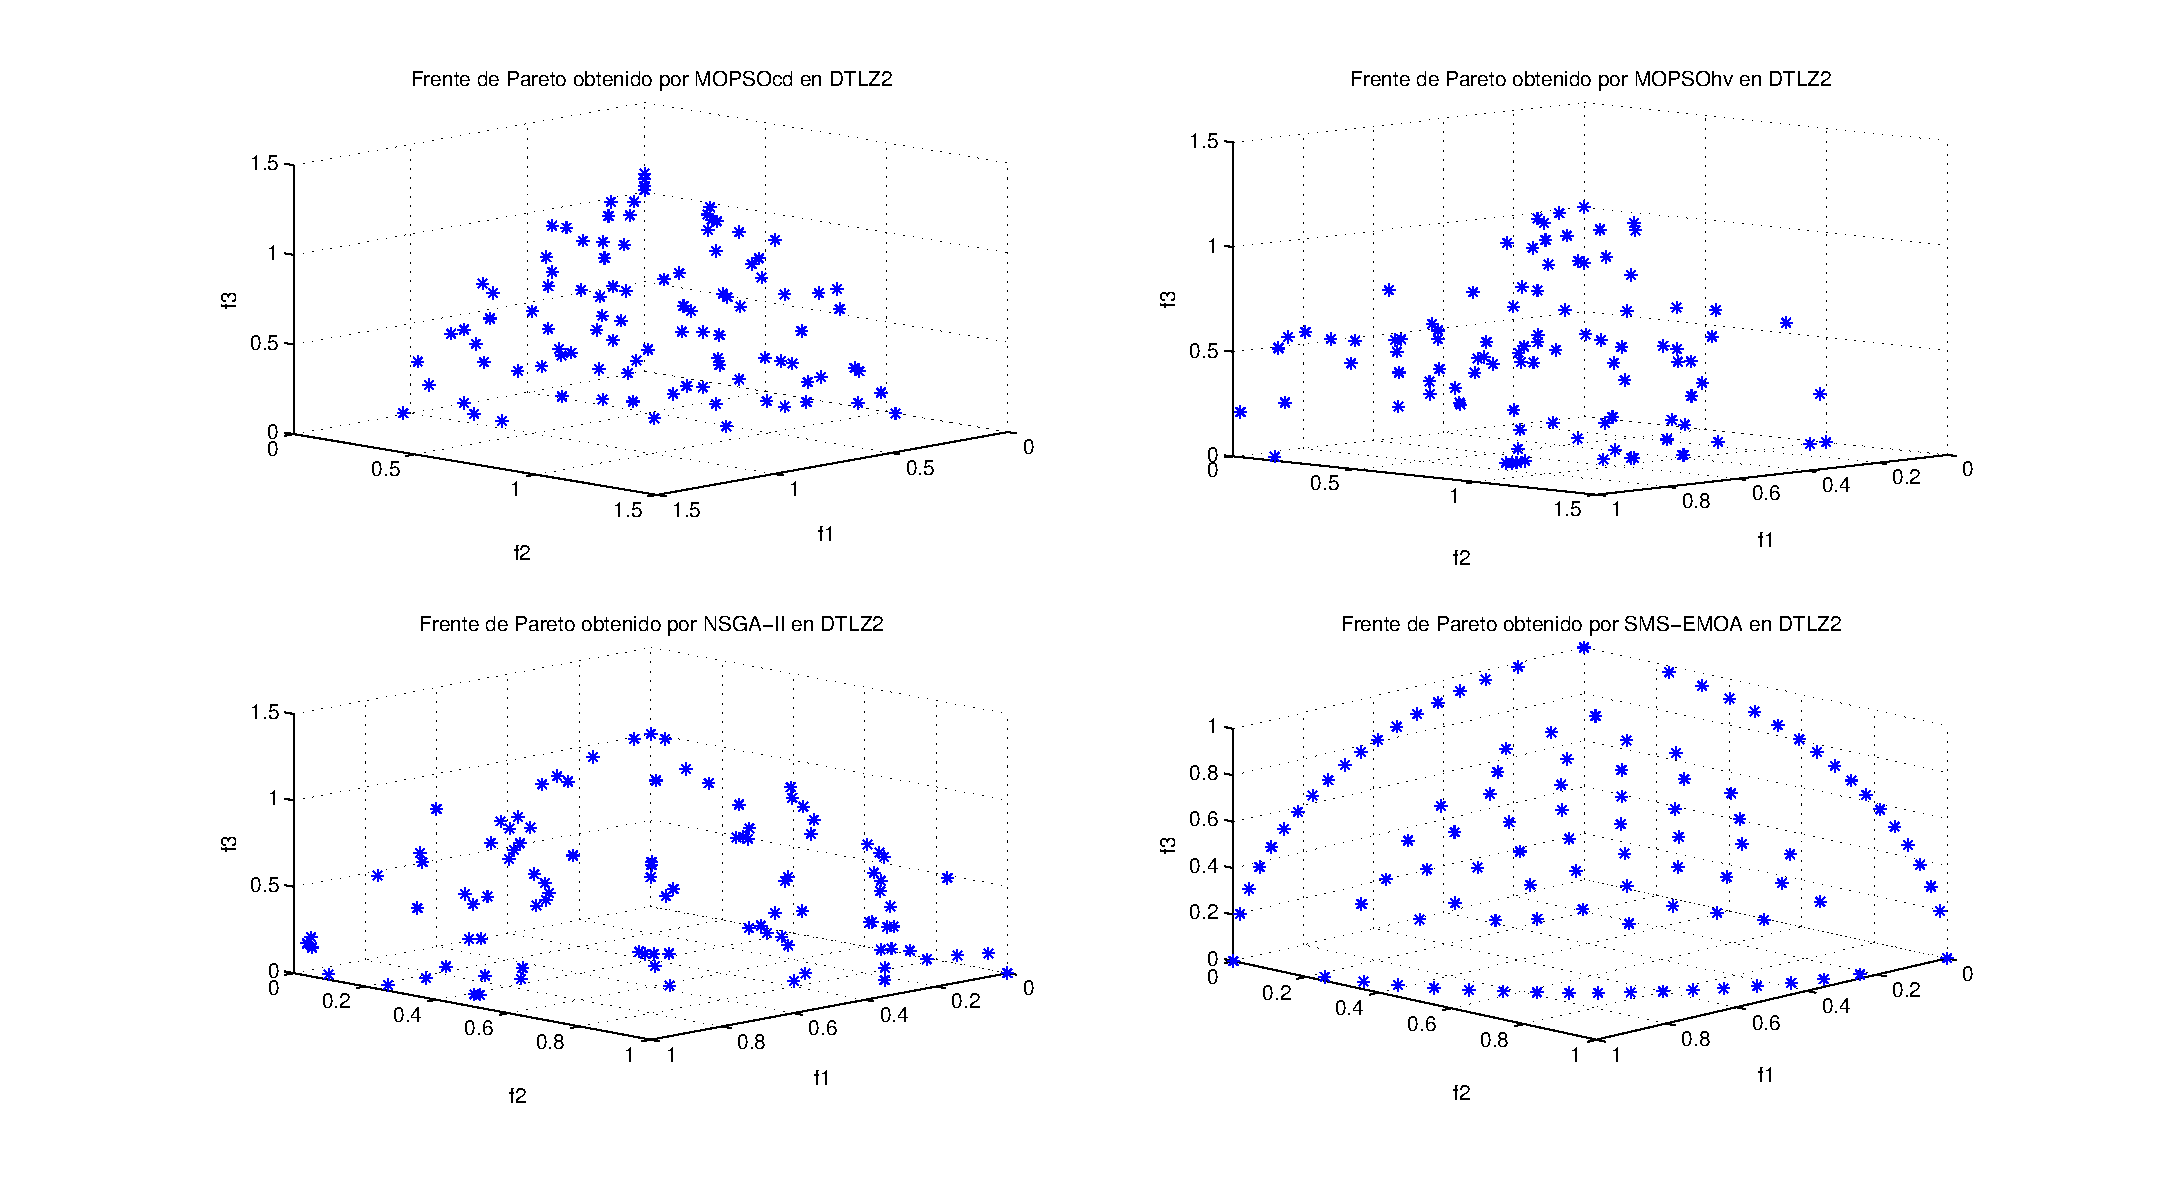
\includegraphics[scale=0.45]{Cap4/rdtlz2r.eps}
      \end{center}
	\caption{Resultados gr\'aficos correspondientes al problema DTLZ2.}
      \label{fig:rDTLZ2}
      \end{figure}

      \clearpage
      \newpage
 
\begin{table}
 \begin{center}
  \begin{tabular}{|l|cc|cc|} \hline
    & \multicolumn{4}{|c|}{Espaciado} \\ 
	\textbf{Algoritmo} & \textbf{Menor} & \textbf{Mayor} & \textbf{Promedio} & \textbf{Desviaci\'on} \\  \hline \hline
	MOPSOhv &0.523852 & 6.539527 & \textbf{\textcolor{green}{ 1.759328}} &  \textbf{\textcolor{red}{1.322038}}    \\ 
	MOPSOcd &0.774392 & 5.346362 & \textbf{\textcolor{red}{ 2.143857}} &  \textbf{\textcolor{green}{0.915538}}   \\ 
	NSGA-II &0.045404 & 0.067297 & \textbf{\textcolor{blue}{ 0.056032}} &  \textbf{0.004531}   \\  
	SMS-EMOA &0.037710 & 0.083937 & \textbf{0.043889} & \textbf{\textcolor{blue}{ 0.009394 }} \\  
	\hline\hline
    & \multicolumn{4}{|c|}{DGI} \\ 
	\hline\hline
	MOPSOhv &0.187750 & 1.484958 & \textbf{\textcolor{green}{ 0.594644}} &  \textbf{\textcolor{green}{0.302257}}   \\ 
	MOPSOcd &0.199480 & 1.812156 & \textbf{\textcolor{red}{ 0.630432}} & \textbf{\textcolor{red}{ 0.323953}}  \\ 
	NSGA-II &0.001123 & 0.001441 & \textbf{0.001235} &  \textbf{0.000083} \\  
	SMS-EMOA &0.015616 & 0.031270 & \textbf{\textcolor{blue}{ 0.016425}} &  \textbf{\textcolor{blue}{0.003406}}  \\  
	\hline\hline
    & \multicolumn{4}{|c|}{Hipervolumen} \\ 
	\hline\hline
	MOPSOhv &0.000000 & 0.000000 & \textbf{\textcolor{green}{ 0.000000 }}& \textbf{\textcolor{green}{ 0.000000 }}\\ 
	MOPSOcd &0.000000 & 0.000000 &  \textbf{\textcolor{red}{0.000000}} & \textbf{\textcolor{red}{ 0.000000 }} \\ 
	NSGA-II &123.004398 & 124.174476 &  \textbf{\textcolor{blue}{123.673815}} &  \textbf{0.295556} \\  
	SMS-EMOA &120.390195 & 124.425951 & \textbf{124.221079} & \textbf{\textcolor{blue}{ 0.878873}}  \\  
	\hline\hline
	& \multicolumn{4}{|c|}{\textbf{Cobertura}} \\ \hline\hline 
	\textbf{Algoritmo} & \textbf{MOPSOhv} & \textbf{MOPSOcd} & \textbf{NSGA-II} & \textbf{SMS-EMOA} \\  \hline \hline
	\textbf{MOPSOhv} &---       & \textbf{0.546000} & \textbf{\textcolor{red}{ 0.000000 }}  &  \textbf{\textcolor{red}{0.000000 }} \\ 
	\textbf{MOPSOcd} & 0.215500 & ---      & 0.000000 & 0.000000 \\ 
	\textbf{NSGA-II} & \textbf{1.000000} & 0.980000 & ---        & 0.052000 \\  
	\textbf{SMS-EMOA}& \textbf{0.960000} & 0.940000 & 0.000000   & --- \\  
	\hline
	\end{tabular}
\caption{Resultados correspondientes al problema DTLZ3.}
  \label{tab:dtlz3}
\end{center}
\end{table}
La multimodalidad de DTLZ3 causa dificultad a nuestra propuesta (MOPSOhv) para converger de manera \'optima, como se muestra en la 
tabla \ref{tab:dtlz3}. En la gr\'afica \ref{fig:rDTLZ3} se muestra que el MOPSOcd y nuestra propuesta no tiene una buena convergencia
al frente de Pareto y no muestran una buena distribuci\'on de las soluciones. Sin embargo, nuestra propuesta domina a las soluciones 
del MOPSOcd. Nuestra propuesta es superada por el SMS-EMOA y NSGA-II y conforme a estos resultados se puede crear una
jerarqu\'ia en orden descendente en t\'erminos de convergencia del conjunto de soluciones pr\'oximas al frente de Pareto real:

\begin{enumerate}
  \item NSGA-II
  \item SMS-EMOA
  \item MOPSOhv
  \item MOPSOcd
\end{enumerate}

\clearpage
\newpage

\begin{figure}
      \begin{center}
	  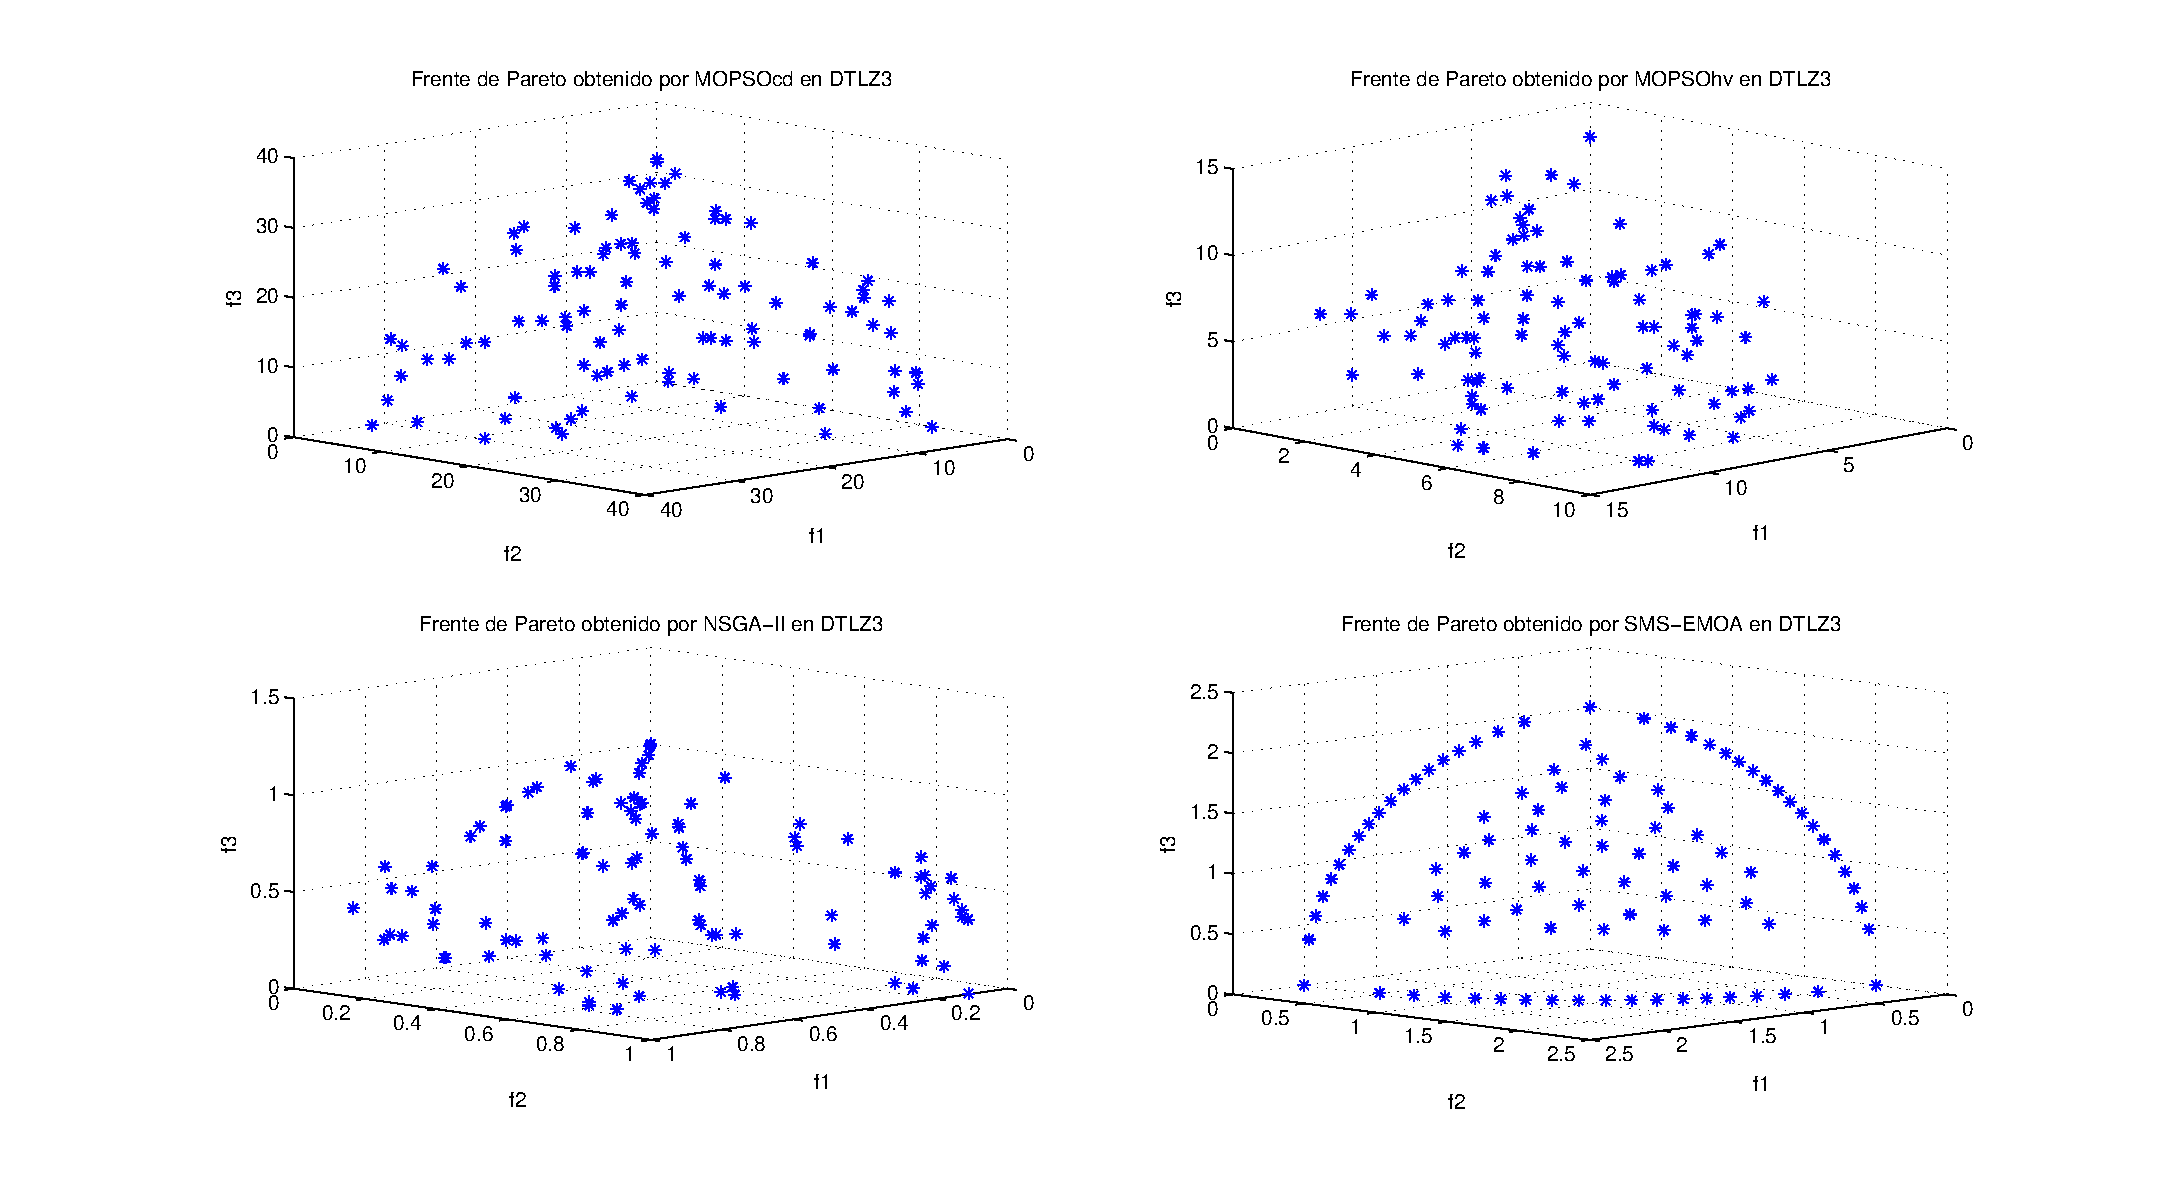
\includegraphics[scale=0.45]{Cap4/rdtlz3r.eps}
      \end{center}
	\caption{Resultados gr\'aficos correspondientes al problema DTLZ3.}
      \label{fig:rDTLZ3}
      \end{figure}

      \clearpage
      \newpage
 

\begin{table}
 \begin{center}
  \begin{tabular}{|l|cc|cc|} \hline
    & \multicolumn{4}{|c|}{Espaciado} \\ 
	\textbf{Algoritmo} & \textbf{Menor} & \textbf{Mayor} & \textbf{Promedio} & \textbf{Desviaci\'on} \\  \hline \hline
	MOPSOhv &0.009443 & 0.080015 & \textbf{\textcolor{blue}{ 0.047999}} & \textbf{\textcolor{red}{ 0.021016}}    \\ 
	MOPSOcd &0.052363 & 0.061539 & \textbf{\textcolor{red}{ 0.056542}} & \textbf{\textcolor{blue}{ 0.002922}}  \\ 
	NSGA-II &0.000000 & 0.063012 &  \textbf{\textcolor{green}{0.051862}} & \textbf{\textcolor{green}{ 0.013087}}   \\  
	SMS-EMOA & 0.039215 & 0.045833 & \textbf{0.042030} & \textbf{ 0.001928}   \\  
	\hline\hline
    & \multicolumn{4}{|c|}{DGI} \\ 
	\hline\hline
	MOPSOhv &0.003982 & 0.010549 &  \textbf{\textcolor{green}{0.006694}} &  \textbf{\textcolor{green}{0.002366}}   \\ 
	MOPSOcd &0.001142 & 0.001271 & \textbf{0.001208} & \textbf{\textcolor{blue}{ 0.000037}} \\ 
	NSGA-II &0.001097 & 0.015257 &  \textbf{\textcolor{blue}{0.001875}} & \textbf{\textcolor{red}{ 0.003071}}   \\  
	SMS-EMOA &0.015606 & 0.015606 & \textbf{\textcolor{red}{0.015606}} &  \textbf{0.000000}   \\  
	\hline\hline
    & \multicolumn{4}{|c|}{Hipervolumen} \\ 
	\hline \hline
	MOPSOhv &0.337305 & 0.666145 &  \textbf{\textcolor{red}{0.548703}} & \textbf{\textcolor{green}{0.117426}} \\ 
	MOPSOcd &0.668445 & 0.708459 &  \textbf{\textcolor{blue}{0.688920}} & \textbf{\textcolor{blue}{ 0.010033}}  \\ 
	NSGA-II &0.121000 & 0.715370 & \textbf{\textcolor{green}{ 0.674632}} & \textbf{\textcolor{red}{ 0.127135}}  \\  
	SMS-EMOA &0.757966 & 0.758160 &\textbf{ 0.758069} & \textbf{0.000050}   \\  
	\hline\hline
	& \multicolumn{4}{|c|}{\textbf{Cobertura}} \\ \hline\hline 
	\textbf{Algoritmo} & \textbf{MOPSOhv} & \textbf{MOPSOcd} & \textbf{NSGA-II} & \textbf{SMS-EMOA} \\  \hline \hline
	\textbf{MOPSOhv} &---       & \textbf{0.189000}   & \textbf{0.013500}   &  \textbf{0.017000} \\ 
	\textbf{MOPSOcd} & 0.000000  & ---       & 0.000500   &  0.000000   \\ 
	\textbf{NSGA-II} & 0.008421  & 0.199500  & ---       &  0.000000  \\  
	\textbf{SMS-EMOA}&  0.000000 & 0.275500  & 0.009500 & --- \\  
	\hline
	\end{tabular}
\caption{Resultados correspondientes al problema DTLZ4.}
  \label{tab:dtlz4}
\end{center}
\end{table}
En el problema DTLZ4 se observa que en las soluciones de nuestra propuesta (MOPSOhv) la distribuci\'on de las soluciones se concentren
en los extremos, causando que existan espacios muy grandes en el centro del frente de Pareto, como se observa en la 
figura \ref{fig:rDTLZ4}, y como consecuencia  el valor de la m\'etrica del hipervolumen disminuya, como se observa en la tabla \ref{tab:dtlz4}. 
Esto puede ser por que nuestra propuesta se concentra en los extremos del frente, ya que estos, pueden
ser aquellas part\'iculas que gu\'ian la b\'usqueda de nuevas solciones, seg\'un su contribuci\'on al hipervolumen. Nuestra propuesta es superada 
por el SMS-EMOA y NSGA-II y conforme a estos resultados se puede crear una jerarqu\'ia en orden descendente en t\'erminos de convergencia del conjunto de 
soluciones pr\'oximas al frente de Pareto real:


\begin{enumerate}
  \item SMS-EMOA
  \item NSGA-II
  \item MOPSOhv
  \item MOPSOcd
\end{enumerate}

Tambi\'en, se observa que en las soluciones de nuestra propuesta dominan a las soluciones de los otros algoritmos.
\clearpage
\newpage

\begin{figure}
      \begin{center}
	  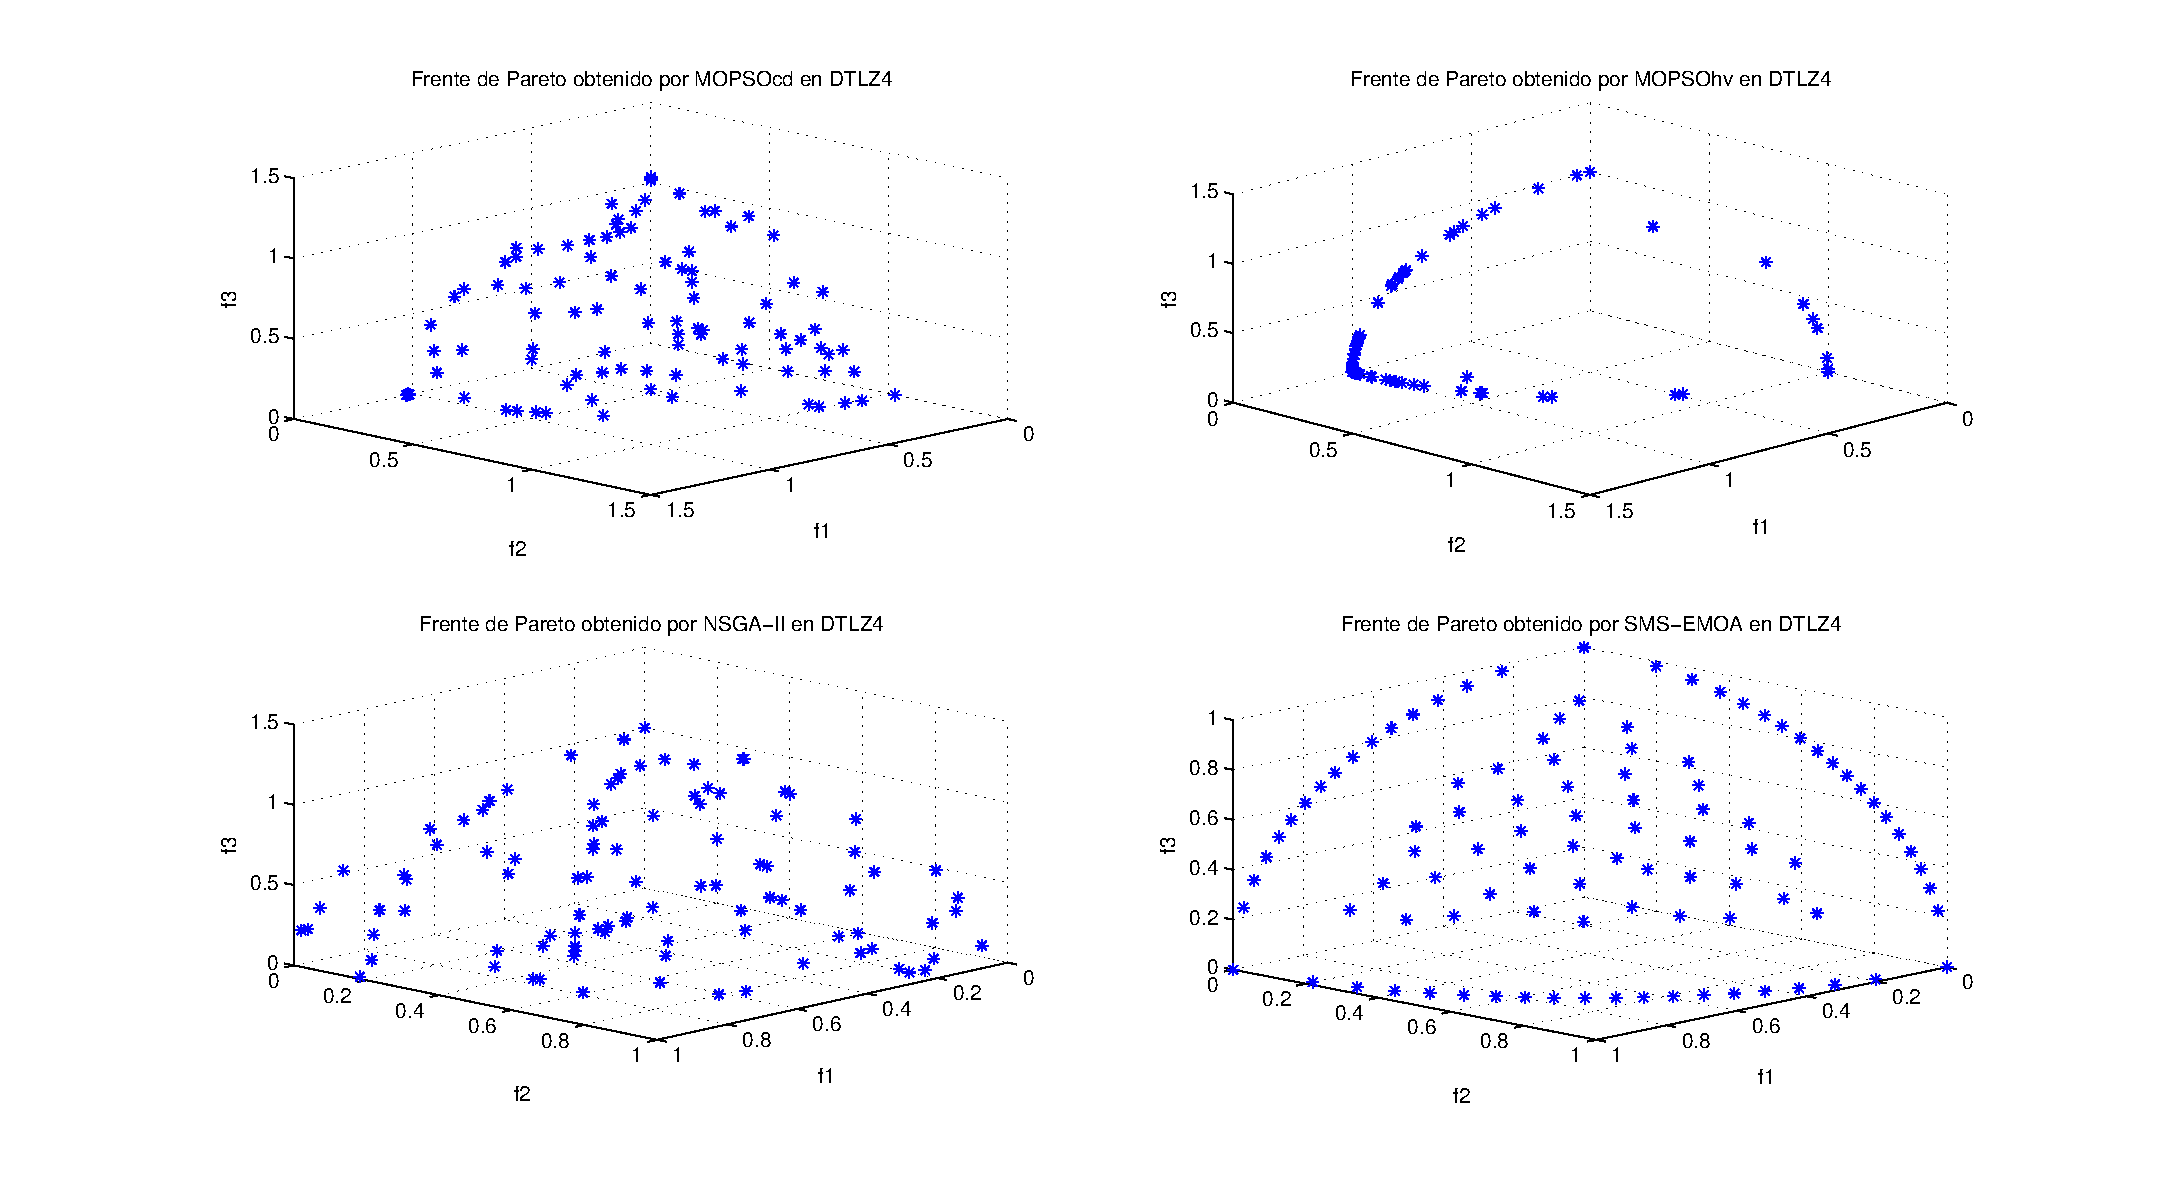
\includegraphics[scale=0.45]{Cap4/rdtlz4r.eps}
      \end{center}
	\caption{Resultados gr\'aficos correspondientes al problema DTLZ4.}
      \label{fig:rDTLZ4}
   \end{figure}

   \clearpage
   \newpage

\begin{table}
 \begin{center}
  \begin{tabular}{|l|cc|cc|} \hline
    & \multicolumn{4}{|c|}{Espaciado} \\ 
	\textbf{Algoritmo} & \textbf{Menor} & \textbf{Mayor} & \textbf{Promedio} & \textbf{Desviaci\'on} \\  \hline \hline
	MOPSOhv &0.009066 & 0.027088 &  \textbf{\textcolor{red}{0.016552}} &  \textbf{\textcolor{blue}{0.005419}}   \\ 
	MOPSOcd &0.007105 & 0.009411 & \textbf{0.008436} & \textbf{\textcolor{green}{ 0.000610 }}  \\ 
	NSGA-II &0.008281 & 0.011557 &  \textbf{\textcolor{green}{0.009727}} &  \textbf{\textcolor{red}{0.000757}}  \\  
	SMS-EMOA &0.008044 & 0.009672 &  \textbf{\textcolor{blue}{0.008763}} &  \textbf{0.000463}  \\  
	\hline\hline
    & \multicolumn{4}{|c|}{DGI} \\ 
	\hline\hline
	MOPSOhv &0.000125 & 0.001589 &  \textbf{\textcolor{green}{0.000439}} & \textbf{\textcolor{red}{ 0.000390}}   \\ 
	MOPSOcd &0.000049 & 0.000058 & \textbf{0.000054} &  \textbf{\textcolor{blue}{0.000002}} \\ 
	NSGA-II &0.000061 & 0.000083 &  \textbf{\textcolor{blue}{0.000069}} &  \textbf{\textcolor{green}{0.000005}}   \\  
	SMS-EMOA &0.009901 & 0.009901 & \textbf{\textcolor{red}{ 0.009901}} &  \textbf{0.000000}   \\  
	\hline
    & \multicolumn{4}{|c|}{Hipervolumen} \\ 
	\hline\hline
	MOPSOhv &0.396024 & 0.435369 &  \textbf{\textcolor{red}{0.428426}} &  \textbf{\textcolor{red}{0.010028}}   \\ 
	MOPSOcd &0.438762 & 0.438946 & \textbf{\textcolor{blue}{0.438852}} &  \textbf{\textcolor{blue}{0.000056}}  \\ 
	NSGA-II &0.437414 & 0.438274 &  \textbf{\textcolor{green}{0.437990}} &  \textbf{\textcolor{green}{0.000223}}  \\  
	SMS-EMOA &0.439348 & 0.439390 & \textbf{0.439374} & \textbf{0.000011}   \\  
	\hline\hline
	& \multicolumn{4}{|c|}{\textbf{Cobertura}} \\ \hline\hline 
	\textbf{Algoritmo} & \textbf{MOPSOhv} & \textbf{MOPSOcd} & \textbf{NSGA-II} & \textbf{SMS-EMOA} \\  \hline \hline
	\textbf{MOPSOhv} &---       & \textbf{0.024500}   &   \textbf{0.024500}  &   \textbf{\textcolor{red}{0.000000}}   \\ 
	\textbf{MOPSOcd} & 0.006500 & ---        &  0.034500 &  0.010000 \\ 
	\textbf{NSGA-II} & 0.020500 &  0.000000  & ---       & 0.010000  \\  
	\textbf{SMS-EMOA}& \textbf{0.000500} &  0.000000  & 0.022000  & --- \\  
	\hline

	\end{tabular}
\caption{Resultados correspondientes al problema DTLZ5.}
  \label{tab:dtlz5}
\end{center}
\end{table}

En el problema DTLZ5 se observa que en nuestra propuesta (MOPSOhv) no tiene una distribuci\'on de las soluciones, lo que causa que existan 
espacios en la aproximaci\'on al frente de Pareto, como se observa en la figura \ref{fig:rDTLZ2}, lo que causa que no se tenga una buena 
cobertura del frente de Pareto, por lo tanto, el valor de la m\'etrica del hipervolumen disminuya, como se observa en la tabla \ref{tab:dtlz2}. 
Nuestra propuesta es superada por el SMS-EMOA y NSGA-II y conforme a estos resultados se puede crear una jerarqu\'ia en orden descendente en t\'erminos de convergencia del conjunto de 
soluciones pr\'oximas al frente de Pareto real:


\begin{enumerate}
  \item NSGA-II
  \item SMS-EMOA
  \item MOPSOcd
  \item MOPSOhv
\end{enumerate}

Tambi\'en, se observa que en las soluciones de nuestra propuesta dominan a las soluciones del NSGA-II y MOPSOcd, y siendo superado por las 
soluciones del SMS-EMOA.

\clearpage
\newpage
 \begin{figure}
      \begin{center}
	  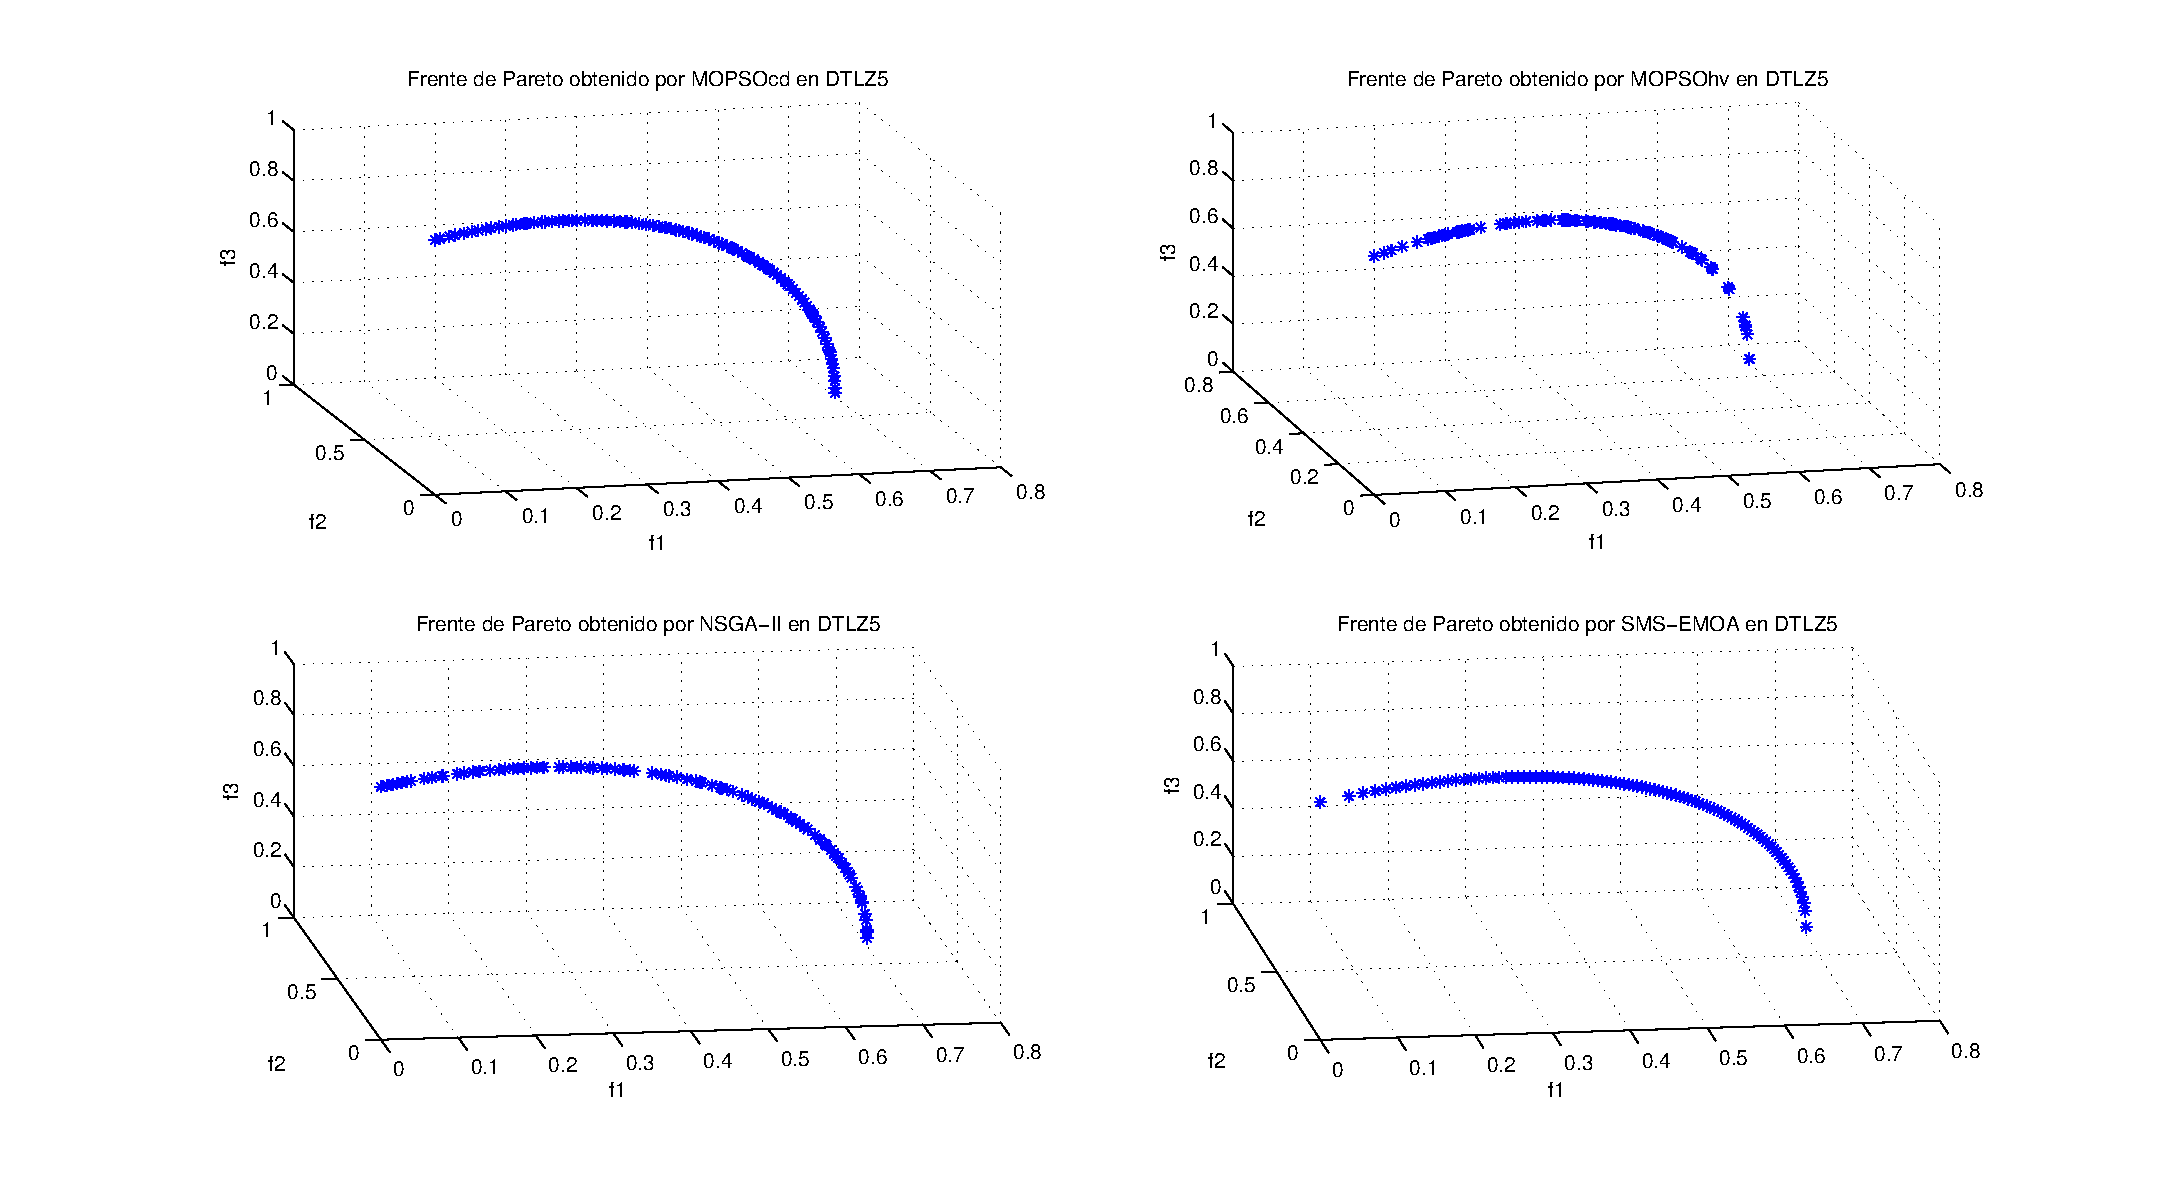
\includegraphics[scale=0.45]{Cap4/rdtlz5r.eps}
      \end{center}
	\caption{Resultados gr\'aficos correspondientes al problema DTLZ5.}
      \label{fig:rDTLZ5}
 \end{figure}
\clearpage
 \newpage
\begin{table}
 \begin{center}
  \begin{tabular}{|l|cc|cc|} \hline
    & \multicolumn{4}{|c|}{Espaciado} \\ 
	\textbf{Algoritmo} & \textbf{Menor} & \textbf{Mayor} & \textbf{Promedio} & \textbf{Desviaci\'on} \\  \hline \hline
	MOPSOhv &0.128037 & 0.220886 &  \textbf{\textcolor{red}{0.158278}} & \textbf{\textcolor{green}{ 0.026187}}   \\ 
	MOPSOcd &0.271101 & 0.501514 &  \textbf{\textcolor{green}{0.343938}} & \textbf{\textcolor{red}{ 0.052728}}   \\ 
	NSGA-II &0.011479 & 0.029482 & \textbf{\textcolor{blue}{ 0.020970}} &  \textbf{\textcolor{blue}{0.004354}}   \\  
	SMS-EMOA & 0.009705 & 0.020519 & \textbf{0.013185} & \textbf{0.002414}  \\  
	\hline\hline
    & \multicolumn{4}{|c|}{DGI} \\ 
	\hline\hline
	MOPSOhv &0.007386 & 0.015926 & \textbf{\textcolor{blue}{ 0.009931}} & \textbf{\textcolor{green}{0.002293}}  \\ 
	MOPSOcd &0.009901 & 0.062068 & \textbf{\textcolor{red}{ 0.036889}} & \textbf{\textcolor{red}{ 0.012547}}  \\ 
	NSGA-II &0.000083 & 0.001194 & \textbf{0.000648} &  \textbf{\textcolor{blue}{0.000236 }}  \\  
	SMS-EMOA &0.010475 & 0.011392 & \textbf{\textcolor{green}{ 0.010786 }}&  \textbf{0.000231 }  \\  
	\hline\hline
    & \multicolumn{4}{|c|}{Hipervolumen} \\ 
	\hline\hline
	MOPSOhv &0.000000 & 0.000616 & \textbf{\textcolor{green}{ 0.000391 }}& \textbf{\textcolor{green}{ 0.000277  }}  \\ 
	MOPSOcd &0.000000 & 0.000000 & \textbf{\textcolor{red}{ 0.000000 }}& \textbf{\textcolor{red}{ 0.000000 }} \\ 
	NSGA-II &0.303244 & 0.437448 & \textbf{0.361529} &  \textbf{\textcolor{blue}{0.028920 }} \\  
	SMS-EMOA &0.282821 & 0.374890 & \textbf{\textcolor{blue}{ 0.340557 }}& \textbf{0.024323 } \\  
	\hline\hline
	& \multicolumn{4}{|c|}{\textbf{Cobertura}} \\ \hline\hline 
	\textbf{Algoritmo} & \textbf{MOPSOhv} & \textbf{MOPSOcd} & \textbf{NSGA-II} & \textbf{SMS-EMOA} \\  \hline \hline
	\textbf{MOPSOhv} & --- &  \textbf{0.920000}       &  \textbf{\textcolor{red}{0.000000}}  &  \textbf{\textcolor{red}{0.000000}} \\ 
	\textbf{MOPSOcd} & 0.000000 & ---       &  0.000000 &  0.000000  \\ 
	\textbf{NSGA-II} & \textbf{0.958000} & 0.996000  & ---       & 0.479500  \\  
	\textbf{SMS-EMOA}& \textbf{0.630000} &  0.640000 & 0.001500  & --- \\  
	\hline
	\end{tabular}
\caption{Resultados correspondientes al problema DTLZ6.}
  \label{tab:dtlz6}
\end{center}
\end{table}
El problema DTLZ6 es muy dificil para nuestra propuesta (MOPSOhv) y el MOPSOcd para converger de manera \'optima, como se muestra en la 
tabla \ref{tab:dtlz6} ya que no logran acerce al frente de Parto, como se muestra en la gr\'afica \ref{fig:rDTLZ6}. Sin embargo, nuestra 
propuesta domina a las soluciones del MOPSOcd. Nuestra propuesta es superada por el SMS-EMOA y NSGA-II y conforme a estos resultados se puede 
crear una jerarqu\'ia en orden descendente en t\'erminos de convergencia del conjunto de soluciones pr\'oximas al frente de Pareto real:

\begin{enumerate}
  \item NSGA-II
  \item SMS-EMOA
  \item MOPSOhv
  \item MOPSOcd
\end{enumerate}

\clearpage
\newpage
\begin{figure}
      \begin{center}
	  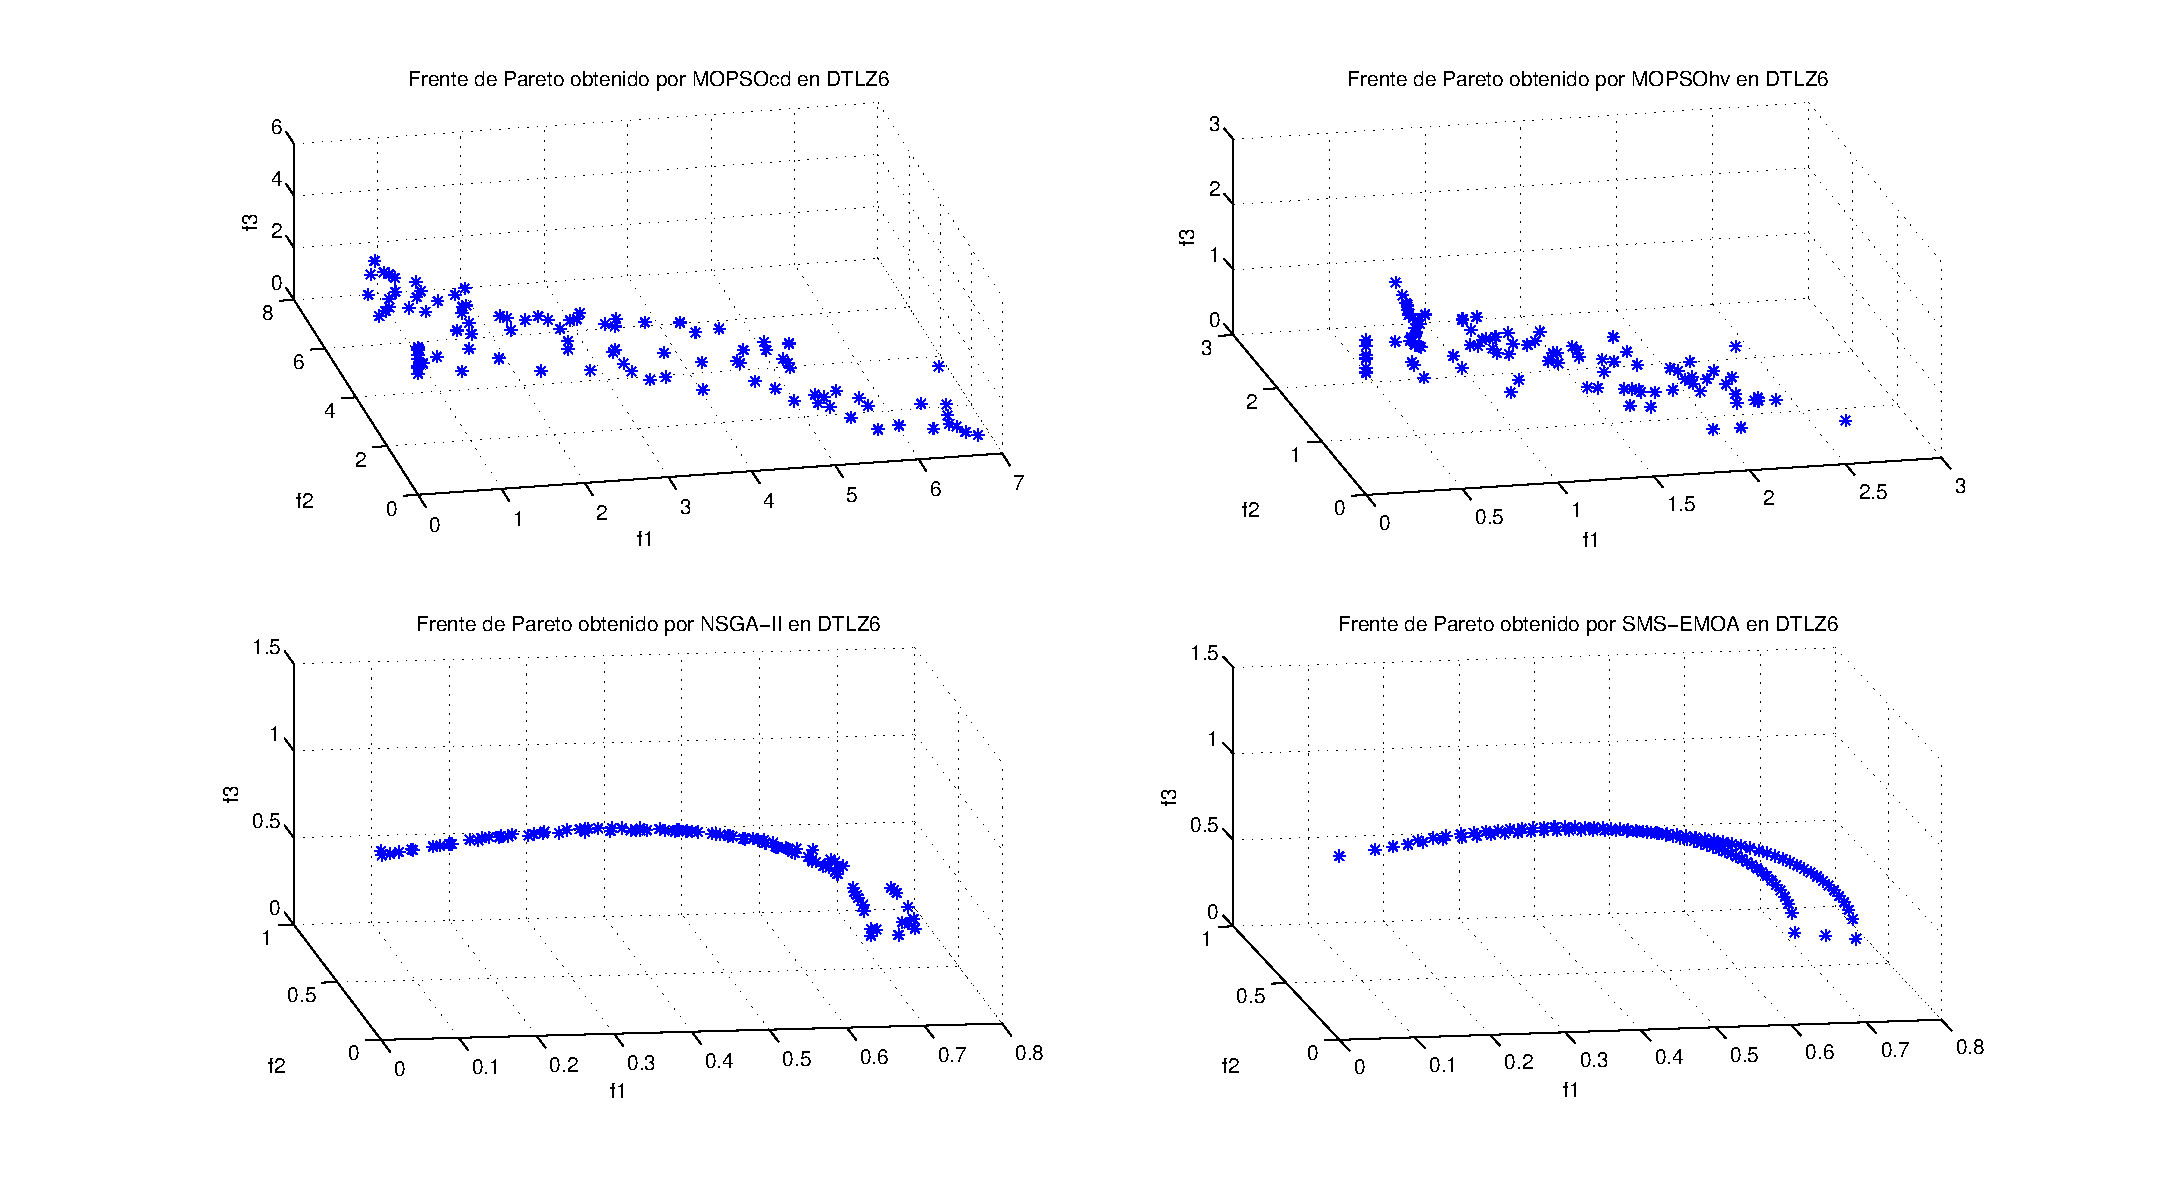
\includegraphics[scale=0.45]{Cap4/rdtlz6r.eps}
      \end{center}
	\caption{Resultados gr\'aficos correspondientes al problema DTLZ6.}
      \label{fig:rDTLZ6}
      \end{figure}
\clearpage
\newpage

 \begin{table}
 \begin{center}
 \begin{tabular}{|l|cc|cc|} \hline
    & \multicolumn{4}{|c|}{Espaciado} \\ 
	\textbf{Algoritmo} & \textbf{Menor} & \textbf{Mayor} & \textbf{Promedio} & \textbf{Desviaci\'on} \\  \hline \hline
	MOPSOhv &0.029933 & 0.140179 &  \textbf{\textcolor{green}{0.085100}} &  \textbf{\textcolor{green}{0.025882}}    \\ 
	MOPSOcd & 0.063885 & 0.453648 &  \textbf{\textcolor{red}{0.114527}} & \textbf{\textcolor{red}{0.112693}}   \\ 
	NSGA-II &0.043496 & 0.085744 &  \textbf{\textcolor{blue}{0.068548}} & \textbf{\textcolor{blue}{0.009758}}  \\  
	SMS-EMOA &0.044055 & 0.063838 & \textbf{0.057420} &  \textbf{0.005603}    \\  
	\hline
    & \multicolumn{4}{|c|}{DGI} \\ 
	\hline\hline
	MOPSOhv &0.001446 & 0.005356 &  \textbf{\textcolor{green}{0.002800}} & \textbf{\textcolor{green}{ 0.001392}}   \\ 
	MOPSOcd & 0.001228 & 0.002112 & \textbf{\textcolor{blue}{0.001558}} &  \textbf{0.000205 }  \\ 
	NSGA-II & 0.000802 & 0.005285 & \textbf{0.001123} &  \textbf{\textcolor{blue}{0.000957}}  \\  
	SMS-EMOA &0.013925 & 0.021469 &  \textbf{\textcolor{red}{0.015064}} & \textbf{\textcolor{red}{ 0.002691}}  \\  
	\hline\hline
    & \multicolumn{4}{|c|}{Hipervolumen} \\ 
	\hline\hline
	MOPSOhv & 2.359510 & 2.812829 &  \textbf{\textcolor{red}{2.608814 }}&  \textbf{\textcolor{green}{0.123164}}  \\ 
	MOPSOcd & 2.430821 & 2.744141 &  \textbf{\textcolor{green}{2.648845 }}&  \textbf{0.072522}   \\ 
	NSGA-II & 2.578211 & 3.011594 &  \textbf{\textcolor{blue}{2.974631 }}&  \textbf{\textcolor{blue}{0.091615}}   \\  
	SMS-EMOA &5.055289 & 5.528637 & \textbf{5.456793} &  \textbf{\textcolor{red}{0.168653}}   \\  
	\hline\hline	
	& \multicolumn{4}{|c|}{\textbf{Cobertura}} \\ \hline\hline 
	\textbf{Algoritmo} & \textbf{MOPSOhv} & \textbf{MOPSOcd} & \textbf{NSGA-II} & \textbf{SMS-EMOA} \\  \hline \hline
	\textbf{MOPSOhv} &---       & \textbf{0.460000}   & \textbf{0.061500} &   \textbf{\textcolor{red}{0.00000}}	 \\ 
	\textbf{MOPSOcd} & 0.003000 & ---       &  0.000000  & 0.000000 \\ 
	\textbf{NSGA-II} & 0.008000 & 0.658500  & ---      &  0.000000    \\  
	\textbf{SMS-EMOA}& \textbf{0.940000} & 0.890000  & 0.980000 & --- \\  
	\hline	
	\end{tabular}
\caption{Resultados correspondientes al problema DTLZ7.}
  \label{tab:dtlz7}
\end{center}
\end{table}
El frente discontinuo de DTLZ7 causa dificultad a nuestra propuesta (MOPSOhv) para converger de manera \'optima, como se muestra en la 
tabla \ref{tab:dtlz7}. En la gr\'afica \ref{fig:rDTLZ7} se muestra que las part\'iculas se concentran en una mayor parte del 
frente de Pareto. Nuestra propuesta es superada por el SMS-EMOA y NSGA-II y conforme a estos resultados se puede crear una
jerarqu\'ia en orden descendente en t\'erminos de convergencia del conjunto de soluciones pr\'oximas al frente de Pareto real:

\begin{enumerate}
  \item NSGA-II
  \item SMS-EMOA
  \item MOPSOhv
  \item MOPSOcd
\end{enumerate}

Tambi\'en, se observa que en las soluciones de nuestra propuesta dominan a las soluciones del NSGA-II y MOPSOcd, y siendo superado por las 
soluciones del SMS-EMOA.
  
  \clearpage

\newpage

\begin{figure}
      \begin{center}
	  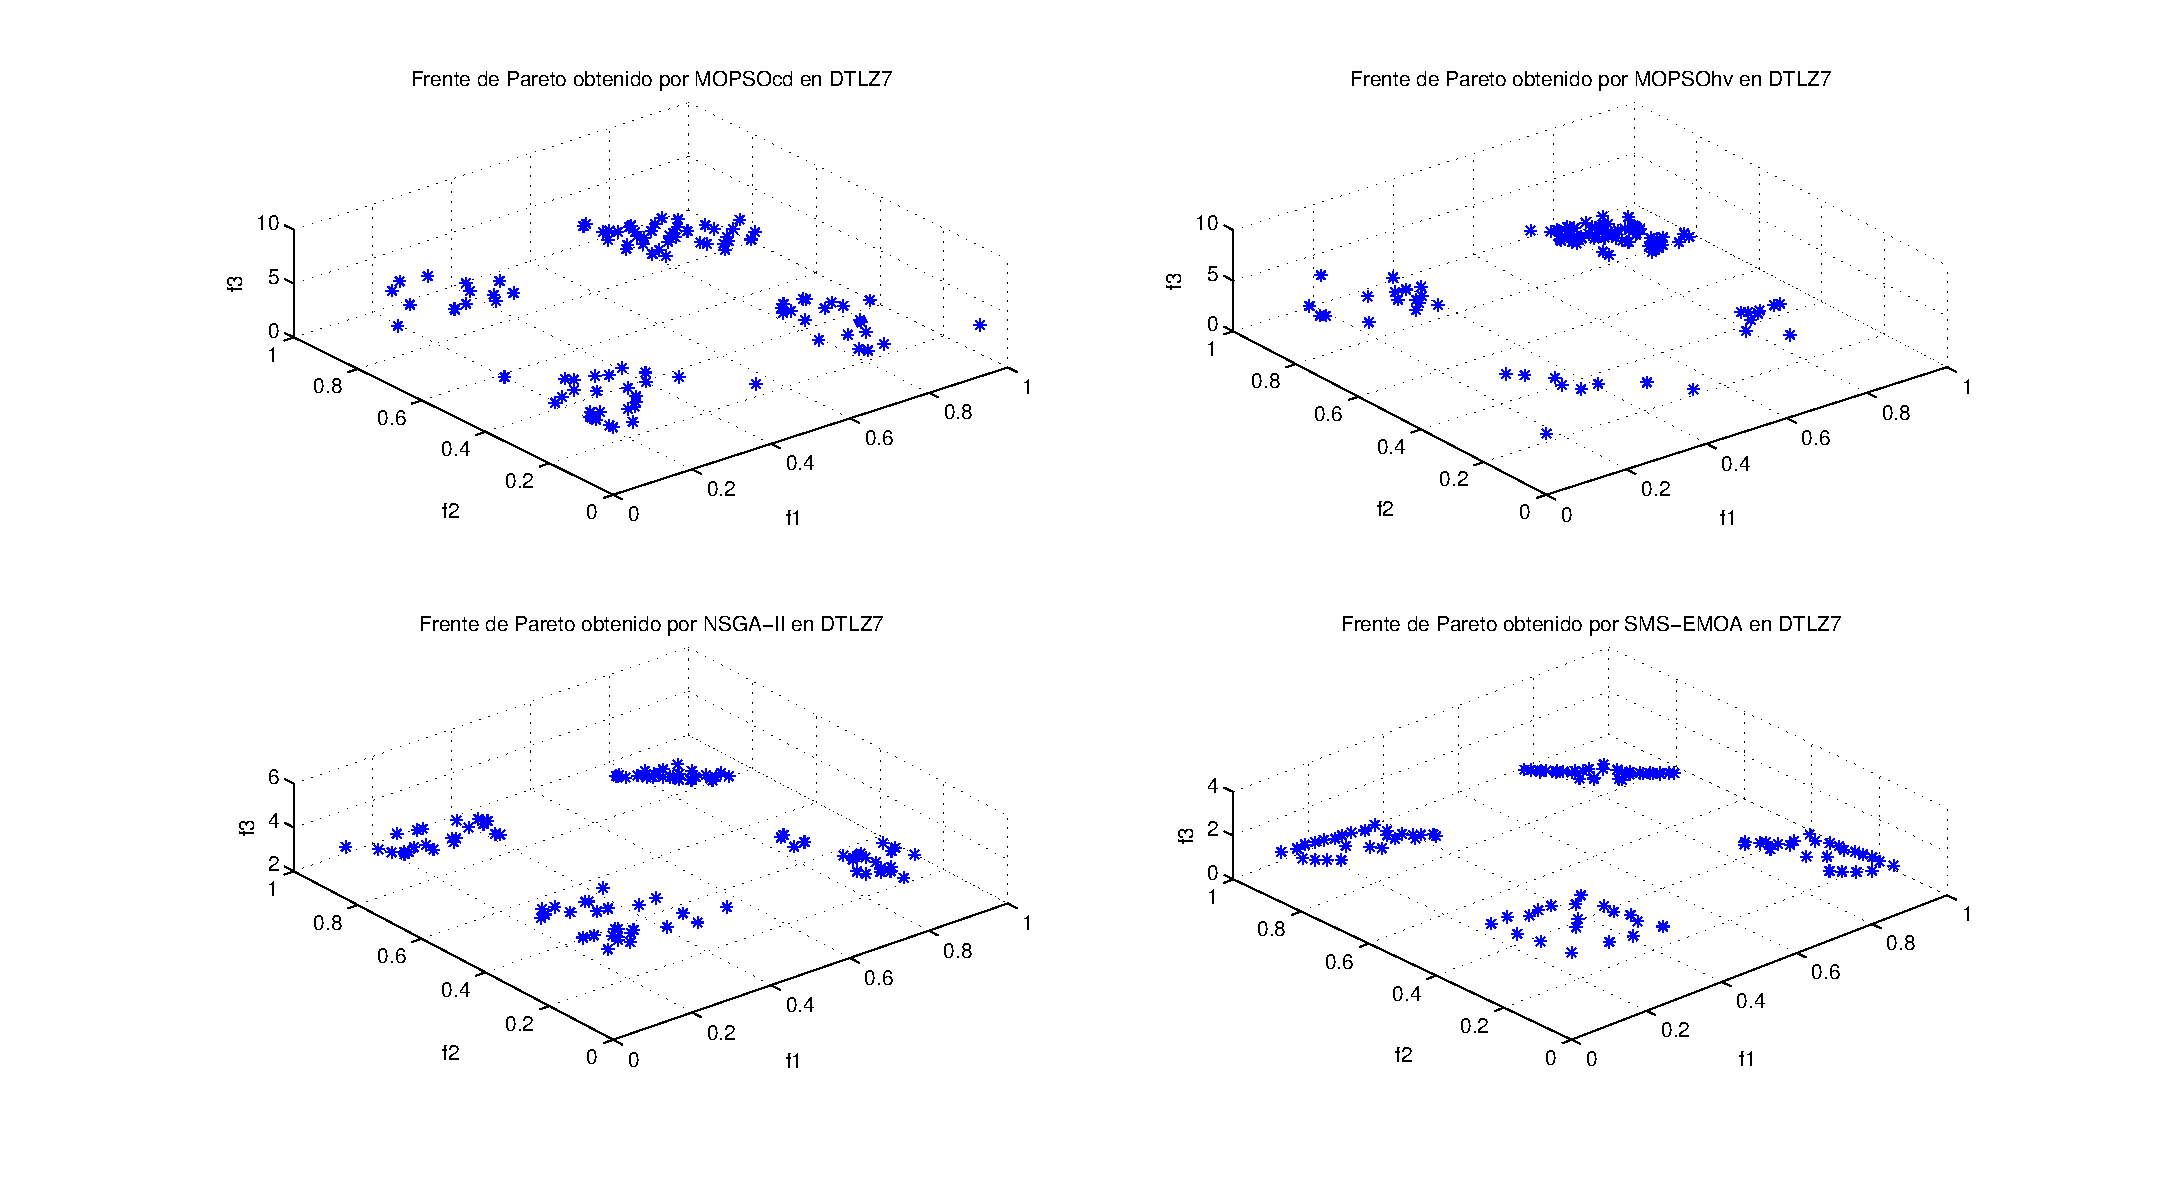
\includegraphics[scale=0.45]{Cap4/rdtlz7r.eps}
      \end{center}
	\caption{Resultados gr\'aficos correspondientes al problema DTLZ7.}
      \label{fig:rDTLZ7}
      \end{figure}
\clearpage


\section{Resultados de escalabilidad}

 Se utiliza el problema DTLZ2 para probar la escalabilidad de nuestro algoritmo de dos a diez objetivos. Las soluciones son comparadas con 
 el NSGA-II, MOPSO-cd y el SMS-EMOA. Se realizaron diez ejecuciones independientes, con 100 individuos y 1200 generaciones usando los 
 par\'ametros de las tablas \ref{tab:parametros1}, \ref{tab:parametros2} y \ref{tab:parametros3}. El punto $\vec{1.1}$ es utlizado como 
 referencia para la m\'etrica del hipervolumen.
 
\begin{longtable}{|l|cc|cc|} 
\hline
    & \multicolumn{4}{|c|}{\textbf{2 Objetivos}} \\ 
	\textbf{Algoritmo} & \textbf{Menor} & \textbf{Mayor} & \textbf{Promedio} & \textbf{Desviaci\'on} \\  \hline \hline
	\textbf{MOPSOhv} & 0.006496 & 0.008450 & \textbf{\textcolor{green}{0.007529}} & \textbf{\textcolor{red}{0.000509}} \\ 
	\textbf{MOPSOcd} & 0.006508 & 0.007755 & \textbf{0.007165} & \textbf{\textcolor{blue}{0.000350}} \\ 
	\textbf{NSGA-II} & 0.006558 & 0.008114 & \textbf{\textcolor{blue}{0.007298}} & \textbf{\textcolor{green}{0.000441}} \\  
	\textbf{SMS-EMOA}& 0.007164 & 0.008134 & \textbf{\textcolor{red}{0.007687}} & \textbf{0.000324}  \\  
	\hline\hline
    & \multicolumn{4}{|c|}{\textbf{3  Objetivos}} \\ 
	\hline\hline
	\textbf{MOPSOhv} & 0.040552 & 0.075311 & \textbf{\textcolor{red}{0.060766}} & \textbf{\textcolor{red}{0.010465}} \\ 
	\textbf{MOPSOcd} & 0.046830 & 0.059367 & \textbf{\textcolor{blue}{0.052755}} & \textbf{\textcolor{blue}{0.003508}} \\ 
	\textbf{NSGA-II} & 0.047551 & 0.062545 & \textbf{\textcolor{green}{0.055653}} & \textbf{\textcolor{green}{0.004653}} \\  
	\textbf{SMS-EMOA}& 0.040739 & 0.045160 & \textbf{0.042945} &\textbf{0.001627} \\
	\hline\hline
    & \multicolumn{4}{|c|}{\textbf{4 Objetivos}} \\ 
	\hline\hline
	\textbf{MOPSOhv} & 0.060814 & 0.103256 & \textbf{\textcolor{blue}{0.076769}} & \textbf{\textcolor{green}{0.013224}} \\ 
	\textbf{MOPSOcd} & 0.255004 & 0.351009 & \textbf{\textcolor{red}{0.307083}} & \textbf{\textcolor{red}{0.029160}} \\ 
	\textbf{NSGA-II} & 0.099124 & 0.121004 & \textbf{\textcolor{green}{0.110590}} & \textbf{\textcolor{blue}{0.007367}} \\  
	\textbf{SMS-EMOA}& 0.060019 & 0.063409 & \textbf{0.061934} & \textbf{0.001271} \\ 
	\hline\hline
 & \multicolumn{4}{|c|}{\textbf{5 Objetivos}} \\ 
	\hline\hline
	\textbf{MOPSOhv} & 0.062663 & 0.115829 & \textbf{0.096073} & \textbf{\textcolor{blue}{0.016611}}    \\ 
	\textbf{MOPSOcd} & 0.357735 & 0.509170 & \textbf{\textcolor{green}{0.439317}} & \textbf{\textcolor{green}{0.048635}} \\ 
	\textbf{NSGA-II} & 0.176407 & 0.213365 & \textbf{\textcolor{blue}{0.194858}} & \textbf{0.012554}  \\  
	\textbf{SMS-EMOA} & --- & --- & \textbf{\textcolor{red}{---}} & \textbf{\textcolor{red}{---}} \\
	\hline\hline
& \multicolumn{4}{|c|}{\textbf{6 Objetivos}} \\ 
	\hline\hline
	\textbf{MOPSOhv} & 0.069909 & 0.146411 & \textbf{0.115437} & \textbf{0.022606}    \\ 
	\textbf{MOPSOcd} & 0.472034 & 0.601704 & \textbf{\textcolor{green}{0.536438}} & \textbf{\textcolor{green}{0.044512}} \\ 
	\textbf{NSGA-II} & 0.326463 & 0.462761 & \textbf{\textcolor{blue}{0.393104}} & \textbf{\textcolor{blue}{0.040260}} \\  
	\textbf{SMS-EMOA} & --- & --- & \textbf{\textcolor{red}{---}} & \textbf{\textcolor{red}{---}} \\
	\hline\hline
 & \multicolumn{4}{|c|}{\textbf{7 Objetivos}} \\ 
	\hline\hline
	\textbf{MOPSOhv} & 0.104604 & 0.198331 & \textbf{0.134378} & \textbf{0.027768}   \\ 
	\textbf{MOPSOcd} & 0.567486 & 0.800344 & \textbf{\textcolor{green}{0.666199}} & \textbf{\textcolor{green}{0.064909}}  \\ 
	\textbf{NSGA-II} & 0.555849 & 0.750226 & \textbf{\textcolor{blue}{0.626970 }}& \textbf{\textcolor{blue}{0.053539}} \\  
	\textbf{SMS-EMOA} & --- & --- & \textbf{\textcolor{red}{---}} &\textbf{\textcolor{red}{ --- }}\\
	\hline\hline
 & \multicolumn{4}{|c|}{\textbf{8 Objetivos}} \\ 
	\hline\hline
	\textbf{MOPSOhv} & 0.091730 & 0.173281 & \textbf{0.122761} & \textbf{0.025681}   \\ 
	\textbf{MOPSOcd} & 0.656487 & 0.898391 & \textbf{\textcolor{blue}{0.768978}} & \textbf{\textcolor{green}{0.083783}} \\ 
	\textbf{NSGA-II} & 0.707636 & 0.843402 & \textbf{\textcolor{green}{0.773139}} & \textbf{\textcolor{blue}{0.048302}} \\ 
	\textbf{SMS-EMOA} & --- & --- &\textbf{\textcolor{red}{ ---}} & \textbf{\textcolor{red}{--- }}\\
	\hline\hline
 & \multicolumn{4}{|c|}{\textbf{9 Objetivos}} \\ 
	\hline\hline
	\textbf{MOPSOhv} &0.069848 & 0.150881 & \textbf{0.109239} & \textbf{0.026673}   \\ 
	\textbf{MOPSOcd} & 0.656487 & 0.898391 & \textbf{\textcolor{blue}{0.768978}} & \textbf{\textcolor{green}{0.083783}} \\ 
	\textbf{NSGA-II} &0.883374 & 0.977749 & \textbf{\textcolor{green}{0.913665}} & \textbf{\textcolor{blue}{0.025785}} \\ 
	\textbf{SMS-EMOA} & --- & --- & \textbf{\textcolor{red}{---}} &\textbf{\textcolor{red}{ ---}} \\
	\hline\hline
 & \multicolumn{4}{|c|}{\textbf{10 Objetivos}} \\ 
	\hline\hline
	\textbf{MOPSOhv} &0.090387 & 0.180091 & \textbf{0.129630} & \textbf{0.028221}    \\ 
	\textbf{MOPSOcd} &0.682277 & 0.953287 & \textbf{\textcolor{blue}{0.826685}} & \textbf{\textcolor{green}{0.093907}}  \\ 
	\textbf{NSGA-II} &0.936894 & 1.132359 & \textbf{\textcolor{green}{1.032422}} & \textbf{\textcolor{blue}{0.071610}}\\  
	\textbf{SMS-EMOA} & --- & --- & \textbf{\textcolor{red}{---}} &\textbf{\textcolor{red}{ ---}} \\
	\hline\hline
\caption{Resultados de la m\'etrica de espaciado para DTLZ2 de 2 a 10 objetivos.}
  \label{tab:dtlz2_es}
\end{longtable}
 
 La tabla \ref{tab:dtlz2_es} muestra como la distribuci\'on de las soluciones mejoran para nuestra propuesta al aumentar el n\'umero 
 de objetivos del problema DTLZ2. Mientras que en el NSGA-II y MOPSOcd el valor de la m\'etrica de espaciado crece al aumentar el n\'umero
 de objetivos nuestra propuesta se mantiene constante.
 
\begin{longtable}{|l|cc|cc|} 
\hline
    & \multicolumn{4}{|c|}{\textbf{2 Objetivos}} \\ 
	\textbf{Algoritmo} & \textbf{Menor} & \textbf{Mayor} & \textbf{Promedio} & \textbf{Desviaci\'on} \\  \hline \hline
	\textbf{MOPSOhv} & 0.420910 & 0.420993 & \textbf{\textcolor{blue}{0.420962}} &\textbf{\textcolor{blue}{ 0.000031}}\\ 
	\textbf{MOPSOcd} & 0.420317 & 0.420437 & \textbf{\textcolor{green}{0.420372}} &\textbf{\textcolor{green}{ 0.000037}}\\ 
	\textbf{NSGA-II} & 0.418849 & 0.419966 & \textbf{\textcolor{red}{0.419588}} &\textbf{\textcolor{red}{ 0.000323}}\\  
	\textbf{SMS-EMOA}& 0.421020 & 0.421027 & \textbf{0.421023} & \textbf{0.000003}\\  
	\hline\hline
    & \multicolumn{4}{|c|}{\textbf{3  Objetivos}} \\ 
	\hline\hline
	\textbf{MOPSOhv} & 0.597900 & 0.697158 & \textbf{\textcolor{red}{0.644946}} & \textbf{\textcolor{red}{0.030303}}\\ 
	\textbf{MOPSOcd} & 0.622449 & 0.698677 & \textbf{\textcolor{green}{0.667862}} & \textbf{\textcolor{green}{0.024190}}\\ 
	\textbf{NSGA-II} & 0.676373 & 0.708493 & \textbf{\textcolor{blue}{0.697689}} & \textbf{\textcolor{blue}{0.009213}}\\  
	\textbf{SMS-EMOA}& 0.757991 & 0.758168 & \textbf{0.758071} & \textbf{0.000056}\\
	\hline\hline
    & \multicolumn{4}{|c|}{\textbf{4 Objetivos}} \\ 
	\hline\hline
	\textbf{MOPSOhv} &0.570237 & 0.735955 & \textbf{\textcolor{green}{0.649871}} & \textbf{\textcolor{green}{0.046065}} \\ 
	\textbf{MOPSOcd} &0.000000 & 0.000000 & \textbf{\textcolor{red}{0.000000}} & \textbf{\textcolor{red}{0.000000}} \\ 
	\textbf{NSGA-II} &0.805413 & 0.876853 & \textbf{\textcolor{blue}{0.834518}} & \textbf{\textcolor{blue}{0.019843}} \\  
	\textbf{SMS-EMOA}&1.044708 & 1.044792 & \textbf{1.044734} & 0.000030 \\ 
	\hline\hline
 & \multicolumn{4}{|c|}{\textbf{5 Objetivos}} \\ 
	\hline\hline
	\textbf{MOPSOhv} &0.526935 & 0.821024 & \textbf{\textcolor{blue}{0.686608}} & \textbf{\textcolor{blue}{0.091850}} \\ 
	\textbf{MOPSOcd} &0.000000 & 0.000000 & \textbf{\textcolor{red}{0.000000}} & \textbf{\textcolor{red}{0.000000}} \\ 
	\textbf{NSGA-II} &0.624795 & 0.874966 & \textbf{0.806271} & \textbf{0.075088}\\  
	\textbf{SMS-EMOA}& --- & --- & \textbf{\textcolor{green}{---}} & \textbf{\textcolor{green}{---}} \\
	\hline\hline
& \multicolumn{4}{|c|}{\textbf{6 Objetivos}} \\ 
	\hline\hline
	\textbf{MOPSOhv} &0.588840 & 0.897113 & \textbf{0.768027} & \textbf{0.106912} \\ 
	\textbf{MOPSOcd} &0.000000 & 0.000000 & \textbf{\textcolor{red}{0.000000}} & \textbf{\textcolor{red}{0.000000}} \\ 
	\textbf{NSGA-II} &0.016168 & 0.385332 & \textbf{\textcolor{blue}{0.195606}} & \textbf{\textcolor{blue}{0.133364}} \\  
	\textbf{SMS-EMOA}& --- & --- & \textbf{\textcolor{green}{---}} &\textbf{\textcolor{green}{ --- }}\\
	\hline\hline
 & \multicolumn{4}{|c|}{\textbf{7 Objetivos}} \\ 
	\hline\hline
	\textbf{MOPSOhv} &0.779870 & 0.986701 & \textbf{0.897171} & \textbf{0.059289} \\ 
	\textbf{MOPSOcd} &0.000000 & 0.000000 & \textbf{\textcolor{red}{0.000000}} & \textbf{\textcolor{red}{0.000000}} \\ 
	\textbf{NSGA-II} &0.000960 & 0.336963 & \textbf{\textcolor{blue}{0.146724}} & \textbf{\textcolor{blue}{0.119704}} \\  
	\textbf{SMS-EMOA} & --- & --- & \textbf{\textcolor{green}{---}} & \textbf{\textcolor{green}{---}} \\
	\hline\hline
 & \multicolumn{4}{|c|}{\textbf{8 Objetivos}} \\ 
	\hline\hline
	\textbf{MOPSOhv} &0.711453 & 1.069716 & \textbf{0.923948} & \textbf{\textcolor{blue}{0.098939}} \\ 
	\textbf{MOPSOcd} &0.000000 & 0.000000 & \textbf{\textcolor{red}{0.000000}} & \textbf{\textcolor{red}{0.000000}} \\ 
	\textbf{NSGA-II} &0.071442 & 0.358558 & \textbf{\textcolor{blue}{0.185958}} & \textbf{0.088435}\\ 
	\textbf{SMS-EMOA} & --- & --- & \textbf{\textcolor{green}{---}} & \textbf{\textcolor{green}{---}} \\
	\hline\hline
 & \multicolumn{4}{|c|}{\textbf{9 Objetivos}} \\ 
	\hline\hline
	\textbf{MOPSOhv} &0.767567 & 1.063881 & \textbf{0.894945} & \textbf{\textcolor{blue}{0.098291}} \\ 
	\textbf{MOPSOcd} &0.000000 & 0.000000 & \textbf{\textcolor{red}{0.000000}} & \textbf{\textcolor{red}{0.000000}} \\ 
	\textbf{NSGA-II} &0.039463 & 0.397496 & \textbf{\textcolor{blue}{0.212041}} & \textbf{0.124973} \\ 
	\textbf{SMS-EMOA} & --- & --- & \textbf{\textcolor{green}{---}} & \textbf{\textcolor{green}{---}} \\
	\hline\hline
 & \multicolumn{4}{|c|}{\textbf{10 Objetivos}} \\ 
	\hline\hline
	\textbf{MOPSOhv} &0.946736 & 1.228404 & \textbf{1.080952} & \textbf{0.085351}   \\ 
	\textbf{MOPSOcd} &0.000000 & 0.000000 & \textbf{\textcolor{red}{0.000000}} & \textbf{\textcolor{red}{0.000000}} \\ 
	\textbf{NSGA-II} &0.015169 & 0.440330 & \textbf{\textcolor{blue}{0.224003}} & \textbf{\textcolor{blue}{0.127577}} \\  
	\textbf{SMS-EMOA} & --- & --- & \textbf{\textcolor{green}{---}} & \textbf{\textcolor{green}{---}} \\
	\hline\hline
\caption{Resultados de la m\'etrica de hipervolumen para DTLZ2 con 2 a 10 objetivos.}
  \label{tab:dtlz2_hv}
\end{longtable}

La tabla \ref{tab:dtlz2_hv} muestra los resultados obtenidos para la m\'etrica del hipervolumen para el problema 
DTLZ2 con 2 a 10 objetivos. El NSGA-II muestra un deterioro en la 
calidad de las soluciones cuando aumenta el n\'umero de objetivos del problema con un costo 
computacional bajo. El SMS-EMOA muestra tener buenos resultados, pero es muy costoso, 
computacionalmente hablando. 
MOPSOcd muestra que su desempe\~no no es escalable ya que se degrada r\'apidamente al aumentar el n\'umero de 
funciones objetivo. 

Conforme a estos resultados se puede crear una
jerarqu\'ia en orden descendente en t\'erminos del valor del hipervolumen del conjunto de soluciones pr\'oximas al frente de Pareto real:

\begin{enumerate}
  \item MOPSOhv
  \item NSGA-II
  \item SMS-EMOA
  \item MOPSOcd
\end{enumerate}

Nuestra propuesta muestra tener buenos resultados en la
calidad de las soluciones cuando aumentan el n\'umero de objetivos del problema al mantenerse constante en la m\'etrica del 
hipervolumen y manteniendo un costo computacional razonable, lo que hace a nuestro algoritmo competitivo respecto a los dem\'as como se muestra en 
la figura \ref{fig:tescala}.

  \begin{figure}
      \begin{center}
	  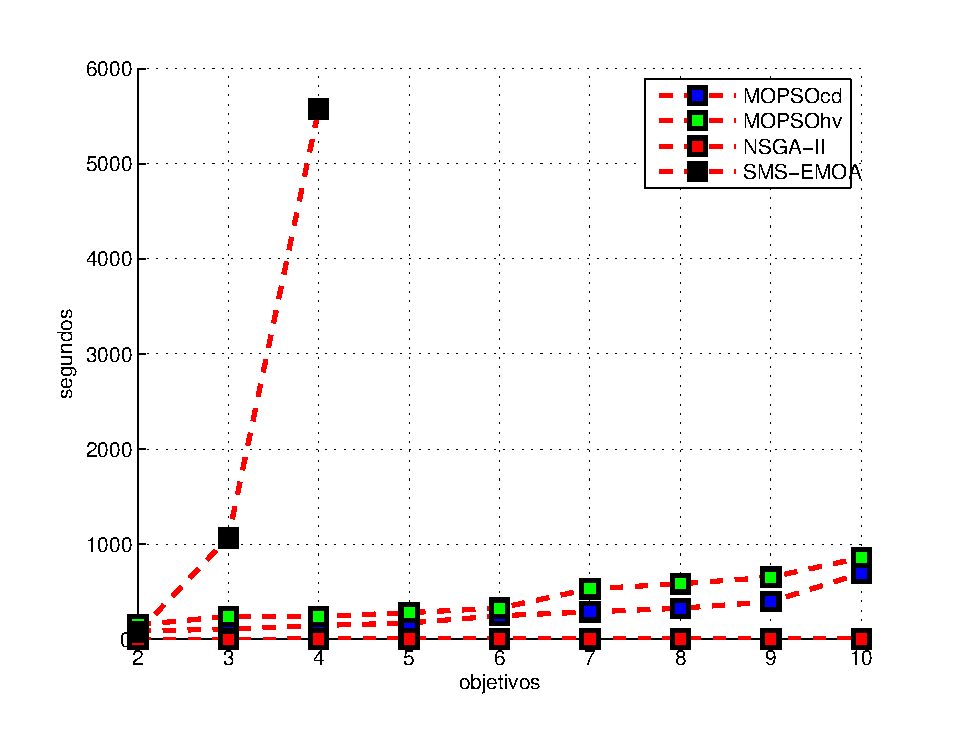
\includegraphics[scale=1]{Cap4/tiempoEscala.eps}
      \end{center}
	\caption[Tiempos en escalamiento para el problema DTLZ2.]{Resultados de tiempo en segundos aumentando el n\'umero 
	de objetivos del problema DTLZ2.}
      \label{fig:tescala}
  \end{figure}

 